%------------------------------%
%% ✎ Dylan (V1) %%%%%%%%% ✅ %%
%% ✎ Alain (V2) %%%%%%%%% ✅ %%
%% ✎ Dylan (V3) %%%%%%%%% ✅ %%
%------------------------------%

%%%%%%%%%%%%%%%%%%%%%%%%%%%%%%%%
% chapter~3
\chapterheader{Doctoral Research Methodology}
\chapter
{A \Commas{Tailor-Made} Survey in the Hauts-de-France Region
    \label{chap3:titre}
    }
    \begin{refsegment}

    % Arrière-plan chapitre~3
    \AddToShipoutPictureBG*{%
\includegraphics[width=\paperwidth,height=\paperheight]{src/Figures/Arriere_plan/Arriere_plan_Chap_3.jpg}
    }

% Rectangle
\AddToShipoutPictureBG*{
  \begin{tikzpicture}[remember picture,overlay]
    \node[fill=white, opacity=0.75, text width=\paperwidth, minimum height=7cm, anchor=north] 
    at ([yshift=-2cm]current page.north) {};
  \end{tikzpicture}
}

% Source
\AddToShipoutPictureFG*{
  \AtPageLowerRight{
    \raisebox{1cm}{
      \hspace{16cm}
      
\begin{tikzpicture}
        \node[fill=white, rounded corners=5pt, inner sep=5pt, align=center] {
          \tiny{Photography: \textcolor{blue}{Dylan Moinse (2022)}}
        };
      \end{tikzpicture}
    }
  }
}

    % ___________________________________________
    % Mini Table of Contents
    \cleardoublepage
    \setcounter{tocdepth}{2}
    % Redefine local table of contents title
    \renewcommand{\localcontentsname}{Table of Contents for Chapter~3}
\localtableofcontents

% Réinitialiser numérotation section
\setcounter{section}{0}

    % ___________________________________________
    % Graphical abstract
    \newpage
\section*{Key Points of Chapter~3
    \label{chap3:graphical-abstract}
    }
    \markright{Chapter Preambule}{}

\begin{figure}[h!]\vspace*{4pt}
        \caption*{}
        \label{graphical-abstract-chap3}
        \centerline{\includegraphics[width=1\columnwidth]{src/Figures/Graphical-abstract/EN_Graphical_abstract_chap3.jpg}}
        \vspace{5pt}
        \begin{flushright}\scriptsize{
        Source: \textcolor{blue}{Morgan Moinse (2022)}
        }\end{flushright}
    \end{figure}

    % ___________________________________________
    % Preamble
    \newpage
    \begin{tcolorbox}[colback=white!5!white,
                      colframe=blue!75!blue,
                      title=
                      \bigskip
                      \center{\textbf{Preamble of Chapter~3}}
                      \\
                      \raggedright{\small{Chapter composed of \pagedifference{chap3:titre}{part1:conclusion} pages, including \pagedifference{chap3:bibliographie}{part1:conclusion} pages of bibliography}}
                      \bigskip]
\Large{\textcolor{blue}{\textbf{Abstract:}}}
    \\
    \small{
This chapter presents the methodology developed to investigate intermodal practices in the train station districts of the Hauts-de-France region. Starting with a contextualization of our case study alongside the description of our mixed research methods, we sought to design a methodology based on a multidimensional and multiscalar approach. Structured into five sections, this chapter successively addresses the definition of the geographical scope, the spatial projection of train station districts, and the implementation of a survey combining quantitative observation, questionnaire administration, and guided tours.%%Translated%%
    \\
The first section defines the geographical boundaries of the study and justifies the choice of the Hauts-de-France region as the analytical framework (see \hyperref[chap3:region-hauts-de-france]{Section~1}, page~\pageref{chap3:region-hauts-de-france}). This choice is based on its dense rail network and its \textsl{a priori} polycentric structure, even though it faces major mobility challenges. Particular attention is given to the reflective stance of the researcher and to ethical considerations.%%Translated%%
    \\
Train station districts are defined as spatial units theoretically accessible on foot or with the use of light individual mobility (see \hyperref[chap3:quartiers-gare]{Section~2}, page~\pageref{chap3:quartiers-gare}). A specific approach, integrating spatial criteria such as acceptable distances and urban environment characteristics, is used to define and map these areas of influence. This approach allows for examining the spatial and functional configuration of these strategic spaces using geostatistical tools.%%Translated%%
    \\
The third section focuses on the quantitative observation of passengers at train stations, particularly users of light individual mobility, who are often underrepresented in public surveys (see \hyperref[chap3:observation-quantitative]{Section~3}, page~\pageref{chap3:observation-quantitative}). The methodological protocol, combining counting and ethnographic observation, is detailed through observation grids applied in nine selected stations.%%Translated%%
    \\
The fourth section discusses the design and administration of a questionnaire targeted at intermodal passengers (see \hyperref[chap3:questionnaire]{Section~4}, page~\pageref{chap3:questionnaire}). It highlights the usefulness of this tool for collecting data on travel practices, perceptions, and expressed needs. The structure of the questionnaire, sampling steps, and response validation are detailed, facilitating the linking of declared movements with geostatistical and behavioral analyses.%%Translated%%
    \\
Finally, the fifth section introduces the approach of guided tours, a qualitative method conducted \textsl{in situ}, allowing for the exploration of user experiences in motion (see \hyperref[chap3:parcours-commente]{Section~5}, page~\pageref{chap3:parcours-commente}). It aims to deepen the understanding of modal choice mechanisms and infrastructure use from the perspective of micro-geographical reports.%%Translated%%
    }
    \tcblower
\Large{\textcolor{blue}{\textbf{Keywords:}}}
    \\
    \small{
Geostatistical analysis;
Hauts-de-France;
Mixed methods;
Quantitative observation;
Research field;
Guided tours;
Questionnaire;
Train station districts
    }
    \end{tcolorbox}

    % ___________________________________________
    % 3.*.
    \newpage
    \needspace{1\baselineskip} % Reserve space
    \addcontentsline{toc}{section}{Introduction of Chapter~3}
    \sectionheader{Introduction of Chapter~3}
\section*{Introduction of Chapter~3
    \label{chap3:introduction}
    }
    \markright{Introduction of Chapter~3}{} 

    % Citation
\begin{displayquote}
\Commas{[\dots] \textsl{through creative processes (ad hoc methods) or synergies (between existing methods), we are able to refine the quality of observation, and then analysis, depending on the case, of a category of daily mobility behaviors or the range of uses of a transport network. The contributions reflect researchers' interest in mobility issues and the great creativity they demonstrate in capturing it.} [\dots] \textsl{To understand this, the analogy with the microscope seems quite telling. Depending on the focal length chosen, the image that a laboratory worker sees forming in the microscope is different each time. However, they are always observing the same reality, but at different scales or, more precisely, from a different perspective. Neither of the images obtained is more true than the other, but they provide a different view of reality.} [\dots] \textsl{Although the complementarity of quantitative and qualitative research is often praised as an ideal, few researchers have actually practiced it to date.} [\dots] \textsl{Methodological innovations and hybridizations are closely linked to the question of researchers' professional practices. Many articles explicitly reference this. These innovations and hybridizations are most often carried out in teams, where each person brings their own practices, skills, and methodological or disciplinary expertise. This collective work, reflected in the contributions gathered here, most of which are written by multiple authors, requires time and coordination to share and implement these know-how within an operational framework. It also requires audacity and creativity to explore experimentation, as well as enough trust, and humility, to (re)acknowledge the values and limits of each method. Finally, it calls for the ability to adapt, to question oneself in response to multiple stimuli from other scientific approaches, different professional viewpoints, or innovations arising from practical uses. Methodological innovations and hybridizations thus appear as a reflection of human creativity, societal progress, and territorial development. It is certainly within this creative and highly collaborative work that the scientific innovations of tomorrow will emerge.}}\footnote{~
    \Commas{[\dots] \textsl{par des processus créatifs (méthodes ad hoc) ou des synergies (entre méthodes déjà existantes), on parvient à affiner la qualité de l’observation, puis de l’analyse, selon le cas, d’une catégorie de comportements de déplacement quotidien ou de l’éventail des usages d’un réseau de transport. Les contributions témoignent de l’intérêt des chercheurs pour les questions de mobilité et de la grande créativité dont ils font preuve pour la saisir.} [\dots] \textsl{Pour le comprendre, l’analogie avec le microscope paraît assez parlante. Selon la focale qu’il choisit, l’image qu’un laborantin voit se former dans le microscope est à chaque fois différente. Il observe pourtant toujours la même réalité, mais à des échelles différentes ou, plus exactement, d’un point de vue différent. Ni l’une ni l’autre des images obtenues n’est plus vraie qu’une autre, mais elles rendent compte d’un regard différent sur la réalité.} [\dots] \textsl{Si la complémentarité des travaux de recherche quantitatifs et qualitatifs est louée de manière récurrente tel un idéal incantatoire, jusqu’à ce jour, peu de chercheurs la pratiquaient dans les faits.} [\dots] \textsl{Les innovations et hybridations méthodologiques renvoient de manière assez directe à la question des pratiques professionnelles des chercheurs. Nombreux sont, du reste, les articles à y faire référence explicitement. Ces innovations et hybridations sont le plus souvent réalisées en équipe, dans lesquelles chacune et chacun apporte ses pratiques, ses savoir-faire et ses compétences méthodologiques ou disciplinaires. Ce travail collectif, qui se reflète dans les contributions rassemblées ici, écrites pour la plupart par plusieurs auteurs, nécessite du temps et de la coordination pour partager les savoir-faire et les mettre en œuvre autour d’un dispositif opérationnalisable. Il nécessite également de l’audace et de la créativité pour pousser la porte de l’expérimentation et suffisamment de confiance, mais aussi d’humilité pour (re)connaître les valeurs et les limites de chaque méthode. Enfin, il suppose une capacité d’adaptation, de remise en question sous l’effet de stimulations multiples venues d’autres approches scientifiques, d’autres points de vue professionnels ou encore d’autres innovations venues des usages. Les innovations et hybridations méthodologiques apparaissent alors comme le reflet des capacités créatives des hommes, de leurs sociétés et de leurs territoires. C’est certainement dans ce travail créatif et fortement collaboratif que se nichent les innovations scientifiques de demain.}} \textcolor{blue}{\autocite[12-14, 160]{meissonnier_connaissance_2020}}\index{Meissonnier, Joël|pagebf}\index{Vincent, Stéphanie|pagebf}\index{Rabaud, Mathieu|pagebf}\index{Kaufmann, Vincent|pagebf}
}

\textcolor{blue}{Joël} \textcolor{blue}{\textcite[12-14, 160]{meissonnier_connaissance_2020}}\index{Meissonnier, Joël|pagebf}\index{Vincent, Stéphanie|pagebf}\index{Rabaud, Mathieu|pagebf}\index{Kaufmann, Vincent|pagebf}. \textsl{Connaissance des mobilités: hybridation des méthodes, diversification des sources}, Éditions du Cerema, Lyon, 176~p. ISBN: \href{https://search.worldcat.org/fr/title/1236011015}{978-2-37180-423-4}
    \end{displayquote}

    % Introduction
\lettrine[lines=3, findent=8pt, nindent=0pt]{\lettrinefont S}{tructuring} of our study is based on the observation of practices and the explanation of intermodal behaviors, with a territorial approach focused on the train station and its surroundings, understood as the interaction of environmental, social, and built dimensions within a single urban system, referencing the concept of \Commas{station interconnection} \textcolor{blue}{\autocite[7]{moretti_interconnexion_1999}}\index{Moretti, Anna|pagebf}\index{Vacheret, Guy|pagebf}. To achieve this, our methodology for studying the stations, their environment, and the practices that unfold within them emphasizes a multidimensional and multiscalar approach. This relational approach articulates three levels of observation: (i) a relational logic, focused on the connection function of network nodes, (ii) a territorial logic, addressing human activities in polarized locations, and (iii) a usage logic, linking space to the behaviors of populations frequenting these nodes \textcolor{blue}{\autocites[9]{moretti_interconnexion_1999}[210-212]{menerault_gares_2001}}\index{Menerault, Philippe|pagebf}\index{Barré, Alain|pagebf}\index{Moretti, Anna|pagebf}\index{Vacheret, Guy|pagebf}. Our ambition is thus to capture the \Commas{territorial accessibility system} in its complexity, by integrating \gls{accessibility} \textsl{of} the territory and \textsl{to} the territory, defined respectively as spatial and social potential, and the interactions between these two dimensions, structured by the geographical space configuration and the characteristics of social groups \textcolor{blue}{\autocite[6]{richer_mesurer_2012}}\index{Richer, Cyprien|pagebf}\index{Palmier, Patrick|pagebf}. We have then leveraged the strengths of both quantitative and qualitative approaches to design an integrated methodological framework \textcolor{blue}{\autocite[]{bergman_advances_2008}}\index{Richer, Cyprien|pagebf}.%%Translated%%

    % Mixed Methods
Rather than opposing them, methods for analyzing movements, whether quantitative or qualitative, would benefit from being considered in a complementary logic \textcolor{blue}{\autocite[6]{klein_mobilites_2007}}\index{Klein, Olivier|pagebf}\index{Ortar, Nathalie|pagebf}\index{Pochet, Pascal|pagebf}. Such an approach implies a more disciplinary sharing focused on the objects of study. In this regard, \textcolor{blue}{\textcite[4]{higgins_forty_2016}}\index{Higgins, Christopher~D.|pagebf}\index{Kanaroglou, Pavlos~S.|pagebf} emphasize the value of combining \Commas{normative} approaches, which qualify the types of \acrshort{TOD}, with \Commas{positive} systematic approaches. It is in this context that the use of various methodological techniques we have implemented is justified, including the exploitation of existing databases combined with observation sessions, questionnaires, and field interviews \textsl{in situ} \textcolor{blue}{\autocite[128]{dureau_lobservation_2014}}\index{Dureau, Françoise|pagebf}\index{Giroud, Matthieu|pagebf}\index{Lévy, Jean-Pierre|pagebf}. The objective of these mixed methods, from a conceptual point of view, is to provide an exploratory basis from \textsl{action captured} through observation. This step allows for the design and adjustment of a questionnaire collecting what is \textsl{signified}. Reported responses are then examined through interviews that capture the experience as it is \textsl{lived and perceived} \textcolor{blue}{\autocite[215]{paugam_enquete_2012}}\index{Paugam, Serge|pagebf}.%%Translated%%

    % Methods Description
The combination of a \Commas{custom} survey, integrating quantitative observation, a questionnaire, and go-along interviews for cycling travelers, aims to provide a comprehensive perspective on a topic that is still under-documented by empirical data (for reference, see \hyperref[fig-introduction:methodes-hypotheses]{Figure~\ref{fig-introduction:methodes-hypotheses}}, in the \hyperref[introduction-generale:methodologie]{general introduction}, page~\pageref{fig-introduction:methodes-hypotheses}). \textcolor{blue}{Joël} \textcolor{blue}{\textcite[24]{meissonnier_pour_2012}}\index{Meissonnier, Joël|pagebf}, as well as \textcolor{blue}{Karel} \textcolor{blue}{\textcite[291]{martens_bicycle_2004}}\index{Martens, Karel|pagebf} for the combined use of \gls{bicycle} and public transport, emphasize the importance of recognizing the limitations of traditional quantitative surveys, such as the \acrfull{PMD}, when it comes to capturing the dynamics of daily mobility, and even more so the chains of movement \textcolor{blue}{\autocite[10]{kieffer_chainage_2011}}\index{Kieffer, Lionel|pagebf}\index{Oliveau, Sébastien|pagebf}\index{Audard, Frédéric|pagebf}. This requires reconsidering the approach by enriching existing databases with field surveys tailored to the demands of our research question. This approach draws on pre-existing work that has paved the way and inspired our methodology. For example, \textcolor{blue}{François de} \textcolor{blue}{\textcite[42]{singly_questionnaire_2016}}\index{Singly, François de|pagebf} highlights the value, in social sciences, of combining the questionnaire, which makes visible the social determinants of trajectories, with interviews, which shed light on the individual construction process of these trajectories. Thus, several studies have demonstrated the value of employing a mixed methodology that combines direct observation, questionnaires, and \Commas{mobile} interviews \textcolor{blue}{\autocites[258]{greene_toward_1989}[120]{bergeron_uncovering_2014}[3]{despres_replacer_2019}}\index{Greene, Jennifer~C.|pagebf}\index{Caracelli, Valerie~J.|pagebf}\index{Graham, Wendy~F.|pagebf}\index{Bergeron, Julie|pagebf}\index{Paquette, Sylvain|pagebf}\index{Poullaouec-Gonidec, Philippe|pagebf}\index{Desprès, Michel|pagebf}\index{Lord, Sébastien|pagebf}\index{Negron-Poblete, Paula|pagebf}.%%Translated%%

    % Outline Announcement 1
The first part of this chapter focuses on defining the geographical area, considered from a macroscopic perspective (\hyperref[chap3:region-hauts-de-france]{Section~1}, page~\pageref{chap3:region-hauts-de-france}). This approach aims to justify the relevance of a regional perspective by presenting the mobility issues as well as the strategic documents established by the competent administrative authority (\hyperref[chap3:regard-privilegie-region-hdf]{Subsection~1.1}, page~\pageref{chap3:regard-privilegie-region-hdf}). In the second part, a sociological self-analysis exercise will be conducted to objectify our positioning in relation to the field, understood both as the subject of research and the geographical context (\hyperref[chap3:auto-analyse-sociologique]{Subsection~1.2}, page~\pageref{chap3:auto-analyse-sociologique}). The description of the geographical scope in which our empirical material is situated will conclude with our relationship to the main mobility manager and the alignment of our survey methods with the principles of research ethics (\hyperref[chap3:preparation-terrain-geographique]{Subsection~1.3}, page~\pageref{chap3:preparation-terrain-geographique}).%%Translated%%

    % Outline Announcement 2
Once the geographical framework is introduced, we will focus on detailing the process of spatializing the train station neighborhoods, understood as spatial units accessible on foot and by light individual mobility, from a microscopic perspective (\hyperref[chap3:quartiers-gare]{Section~2}, page~\pageref{chap3:quartiers-gare}). We will define the methodological rules for mapping these influence areas, based on the distances deemed acceptable and the typology of the stations, as determined through our field survey (\hyperref[chap3:quartiers-gare-distances]{Subsection~2.1}, page~\pageref{chap3:quartiers-gare-distances}). Once the sizes of the station neighborhoods are defined, our attention will shift to their shapes and boundaries, influenced by the characteristics of the built environment. This step will include a reflection on the methods used to generate and represent these shapes (\hyperref[chap3:quartiers-gare-formes]{Subsection~2.2}, page~\pageref{chap3:quartiers-gare-formes}). To conclude this section, we will present the principles for extracting and processing the geostatistical data we have set for ourselves. We will outline the criteria used to exploit the databases, aiming to achieve a high degree of resolution in geographic information (\hyperref[chap3:quartiers-gare-analyse-geostatistique]{Subsection~2.3}, page~\pageref{chap3:quartiers-gare-analyse-geostatistique}).%%Translated%%

    % Outline Announcement 3
The third section of our methodological chapter will be dedicated to describing the quantitative observation approach for cycling travelers, with the aim of providing an overall overview and evaluating current trends, which are still under-documented (\hyperref[chap3:observation-quantitative]{Section~3}, page~\pageref{chap3:observation-quantitative}). First, we will define what constitutes quantitative observation, explaining its relevance to some of our research objectives (\hyperref[chap3:observation-quantitative-outil-adapte]{Subsection~3.1}, page~\pageref{chap3:observation-quantitative-outil-adapte}). Then, we will detail the methodological protocol of our approach, combining counting and ethnographic observation. We will present the observation grid used and the methods for its implementation (\hyperref[chap3:methodologie-observation-quantitative]{Subsection~3.2}, page~\pageref{chap3:methodologie-observation-quantitative}). The section concludes with the contextualization of the nine stations examined in this survey, where we will justify their selection (\hyperref[chap3:observation-quantitative-gares-examinees]{Subsection~3.3}, page~\pageref{chap3:observation-quantitative-gares-examinees}).%%Translated%%

    % Outline Announcement 4
Following the quantitative observation, we will introduce the questionnaire addressed to users (\hyperref[chap3:questionnaire]{Section~4}, page~\pageref{chap3:questionnaire}). We will emphasize the added value of this methodological tool (\hyperref[chap3:apports-questionnaire-usagers]{Subsection~4.1}, page~\pageref{chap3:apports-questionnaire-usagers}). We will then detail the process of administering the questionnaire, presenting its general structure, the sampling process, and the validation of the responses obtained, which have allowed the declared movements to be projected (\hyperref[chap3:administration-questionnaire-usagers]{Subsection~4.2}, page~\pageref{chap3:administration-questionnaire-usagers}).%%Translated%%

    % Outline Announcement 5
The third approach of our field survey, which will be presented throughout this thesis, is based on an initial exploration of go-along interviews (\hyperref[chap3:parcours-commente]{Section~5}, page~\pageref{chap3:parcours-commente}). First, we will place this in-situ interview method in context, emphasizing its different variations (\hyperref[chap3:parcours-commente-definition]{Subsection~5.1}, page~\pageref{chap3:parcours-commente-definition}). Then, we will show how this method was adapted to our field of study, through the \Commas{micro-geographical} reports generated (\hyperref[chap3:parcours-commente-administration-participants]{Subsection~5.2}, page~\pageref{chap3:parcours-commente-administration-participants}).%%Translated%%

    % Outline Announcement 6
In conclusion, we will place the various approaches within an overarching view, to illustrate their articulation and connection with our research hypotheses (\hyperref[chap3:conclusion]{Chapter~3 conclusion}, page~\pageref{chap3:conclusion}).%%Translated%%

     % ___________________________________________
    % 3.1.
    \newpage
    \needspace{1\baselineskip} % Reserve space
    \sectionheader{Contextualization of the Hauts-de-France Region}
\section{Defining the Geographical Area Bound by the Hauts-de-France Region
    \label{chap3:region-hauts-de-france}
    }

    % Introduction
Entering the field requires first and foremost justifying the choice of this boundary and placing it in its context to understand its local characteristics and territorial challenges. This approach also involves introspection on our own personal and ethical relationship to the places explored and the people interviewed. This first section thus aims to define the geographical framework of our empirical research, while explaining the foundations of our methodological stance. A study from the \acrshort{TOD} perspective reveals its full value when it is part of a regional approach, with the goal of establishing a comprehensive vision for regional development \textcolor{blue}{\autocite[24]{lo_feudo_scenario_2014}}\index{Lo Feudo, Fausto|pagebf}\index{Menerault, Philippe|pagebf}\index{L'Hostis, Alain|pagebf}\index{Festa, Demetrio Carmine|pagebf}. Public transport, and more specifically rail, is a structuring lever for regional planning, perceived in Hauts-de-France as a \Commas{spatial capital offering multiple opportunities} \textcolor{blue}{\autocite[147, 163]{baron_reseaux_2017}}\index{Baron, Nacima|pagebf}\index{Messulam, Pierre|pagebf}. As evidenced by the guidelines defined by \textcolor{blue}{\textcite[17]{region_hauts-de-france_planification_2024}}\index{Région Hauts-de-France@\textsl{Région Hauts-de-France}|pagebf}, which aim to \Commas{\textsl{make the regional transport network the backbone of mobility in Hauts-de-France} [\dots] \textsl{focusing primarily on the regional structuring network (rail and road lines)} [\dots] [with a system of] \textsl{feeders to these modes through relevant alternatives}}.%%Translated%%

% Announcement of the plan
First, we will begin by explaining and describing the situation and challenges of the Hauts-de-France region, which serves as the geographical framework for this research (see the \hyperref[chap3:regard-privilegie-region-hdf]{section on the privileged perspective on the Hauts-de-France region}, page~\pageref{chap3:regard-privilegie-region-hdf}). Through this detailed exploration of the regional territory, we will have the opportunity to establish a scientific objectification stance supported by a method of \Commas{sociological self-analysis} (see the \hyperref[chap3:auto-analyse-sociologique]{section on sociological reflexivity}, page~\pageref{chap3:auto-analyse-sociologique}). We will also address the ethical aspects of our empirical research by describing the actions taken to ensure adherence to these principles in our interactions with local actors and the territories involved (see the \hyperref[chap3:preparation-terrain-geographique]{section on research ethics compliance}, page~\pageref{chap3:preparation-terrain-geographique}).%%Translated%%

% 3.1.1.
\needspace{1\baselineskip} % Reserve space
\subsection{Action Research and Public Policy Territories: A Privileged Perspective on the Hauts-de-France Region
    \label{chap3:regard-privilegie-region-hdf}
    }

    % Introduction
In the French context, and for most geographers, the region is often considered the fundamental territorial unit in the functioning of the globalized economic system \textcolor{blue}{\autocite[]{calthorpe_regional_2001}}\index{Calthorpe, Peter|pagebf}\index{Fulton, William|pagebf}. However, this conception raises an important question: are we referring to an \textsl{urban} or \textsl{functional} region, in terms of daily flows, or a \textsl{political} region, defined by administrative divisions? Situated within the ecological and connected transition program \textsl{rev3} (\textsl{Third Industrial Revolution})\footnote{~
    The 21\textsuperscript{st} century is marked by the \textsl{Third Industrial Revolution}, as referenced in the work by economist \textcolor{blue}{Jeremy} \textcolor{blue}{\textcite[338]{rifkin_troisieme_2012}}\index{Rifkin, Jeremy|pagebf}, one of whose five pillars is the emergence of a digital and electrical economy, partly expressed through the sharing of connected transportation. For the author, the \textsl{Third Industrial Revolution} disrupts traditional ways of thinking about and practicing urban mobility. It is within this framework that the author was consulted to devise a roadmap for the Hauts-de-France region. The acronym \textsl{rev3}, led by the Region and the \acrfull{CCI} Hauts-de-France, refers to this policy in the Hauts-de-France that proposes models for territorial and mobility development toward 2050.
}, the present doctoral project could legitimately focus on the institutional region. However, other arguments support the deliberate choice to concentrate on the administrative region, as developed in the doctoral thesis of \textcolor{blue}{Julia} \textcolor{blue}{\textcite[166]{frotey_acteurs_2021}}\index{Frotey, Julia|pagebf}\index{Deboudt, Philippe|pagebf}\index{Castex, Élodie|pagebf}\index{Frère, Séverine|pagebf} on the development of electromobility in the Hauts-de-France. Historically, geography has sought to distance itself from political divisions in order to better understand the complexity of spatial functioning, considering the flows and exchanges that traverse them \textcolor{blue}{\autocite[]{pumain_regionalisation_2016}}\index{Pumain, Denise|pagebf}. This distancing, particularly prominent after the war—\textcolor{blue}{\textcite[16-18]{menerault_reseaux_1991}}\index{Menerault, Philippe|pagebf}\index{Dupuy, Gabriel|pagebf} referred to it as \Commas{eclipse} in his doctoral work—began to fade in the 1970s, when political geography regained an interest in territories, viewed as forms of spatial organization linked to public action.%%Translated%%

% Regional geography
More broadly, this reflection on the institutional regional scale is part of regional geography. It resonates with the long process of decentralization initiated in France, as well as the recent context of regional mergers. As \textcolor{blue}{Nicole} \textcolor{blue}{\textcite[107]{girard_region_2004}}\index{Girard, Nicole|pagebf} recalls, geography is \Commas{\dots \textsl{perhaps one of the most 'regionalized' academic disciplines, in the sense that, for a long time, its regional implantation has been asserted} \dots}. In France, the concept of \Commas{region} is now primarily associated with the politico-administrative framework, thus distancing itself from the \Commas{natural region}, where human-environment relations occur, a concept dear to Vidalian geography and the French School of Geography \textcolor{blue}{\autocite[391]{mercier_entre_2001}}\index{Mercier, Guy|pagebf}. In this regard, the region, as a politico-administrative and spatial entity, is gradually becoming an undeniable reality for both citizens and researchers \textcolor{blue}{\autocite[111]{girard_region_2004}}\index{Girard, Nicole|pagebf}. For these reasons, this thesis adopts the administrative scale of the region as the geographical reference, allowing us to rely on an institutional scale suitable for our research topic, positioned at the heart of the hierarchy of scales, and to access open databases, which are sometimes difficult to find otherwise.%%Translated%%

% 3.1.1.1.
\needspace{1\baselineskip} % Reserve space
\subsubsection*{Interest of a Regional Approach to \textsl{Transit-Oriented Development}
    \label{chap3:approche-regionale}
    }

    % TOD and train
\textcolor{blue}{Peter} \textcolor{blue}{\textcite[62, 67, 104]{calthorpe_next_1993}}\index{Calthorpe, Peter|pagebf} fundamentally distinguishes two geographical scales for the application of \acrshort{TOD}: one at an interurban or regional level, and the other focused on the \Commas{neighborhood}, giving this planning concept a multiscalar dimension. This approach reflects the influence of the \textsl{Smart Growth} movement, which promotes planning focused on regional urbanization development \textcolor{blue}{\autocite[70]{dushina_tod_2015}}\index{Dushina, Anna|pagebf}\index{Paulhiac, Florence|pagebf}\index{Scherrer, Franck|pagebf}. The question of the geographical scale of \acrshort{TOD} application is crucial. Indeed, limiting the analysis to a single station neighborhood excludes the multiscalar logic of connectivity at broader scales \textcolor{blue}{\autocite[273]{menerault_gares_2001}}\index{Menerault, Philippe|pagebf}\index{Barré, Alain|pagebf}. A regional approach thus places \acrshort{TOD} within a polycentric planning perspective\footnote{~
    A broad scientific debate questions the often-attributed virtues of polycentric urban systems in reducing carbon mobility flows, particularly long daily trips. \textcolor{blue}{\textcite[515]{richardson_discourses_2000}}\index{Richardson, Tim|pagebf}\index{Jensen, Ole~B.|pagebf} refer to a \Commas{spatial narrative} to describe the orientations of European planning policies in favor of polycentric territorial configurations. These policies promote polycentrism, which relies on an urban organization with multiple centers or hubs of activity. This model is supposed to reduce long-distance travel, typically done by car, by bringing residents closer to their workplaces, essential services, and economic opportunities. Furthermore, it allows for a better distribution of mobility flows and optimization of transport networks through the combination of radial networks and inter-hub belts. This model also contributes to better territorial equity, by reducing access disparities from peripheral areas. However, empirical research, such as that by \textcolor{blue}{Anne} \textcolor{blue}{\textcite[1545]{aguilera_growth_2005}}\index{Aguiléra, Anne|pagebf} for Paris, Lyon, and Marseille; or by \textcolor{blue}{Florent} \textcolor{blue}{\textcite{le_nechet_modelling_2019}}\index{Le Néchet, Florent|pagebf} for Île-de-France and the Ruhr, shows that polycentric systems, by dispersing mobility flows, complicate the planning of public transport networks, which are often less efficient than in a monocentric model where flows converge toward a single center. Moreover, the governance of these systems proves complex due to the inter-territorial issues they entail. Finally, polycentrism may generate a rebound effect, fostering inter-hub commuting practices and, paradoxically, an overall increase in travel.
}, which is more coherent in the deployment of alternative mobility systems, such as the rail system, which is relevant in the European context \textcolor{blue}{\autocite[212]{bertolini_sustainable_2005}}\index{Bertolini, Luca|pagebf}\index{Le Clercq,~F.|pagebf}\index{Kapoen,~L.|pagebf}. In practice, \acrshort{TOD} is indeed interpreted differently depending on geographical contexts. In the United States, \acrshort{TOD} projects deployed in metropolitan areas focus on \Commas{light} infrastructures such as trams or \acrfull{BRT} systems, while in Europe, particularly in France, the rail system is better suited to a regional scale \textcolor{blue}{\autocite[95]{bonin_evaluation_2015}}\index{Bonin, Olivier|pagebf}\index{Tomasoni, Lorenza|pagebf}. For example, \textcolor{blue}{Alexis} \textcolor{blue}{\textcite[132]{conesa_accessibility_2018}}\index{Conesa, Alexis|pagebf} illustrates, in the case of the former Nord-Pas-de-Calais region, how certain local accessibility gaps can be mitigated by strengthening the connectivity of the station to the network, thanks to the regional reach of \acrshort{TOD}.%%Translated%%

% TOD and urban region
The choice of a regional scale allows for placing train stations within a broader urban development dynamic. The central hypothesis in regional research on \acrshort{TOD} is based on an approach aiming to articulate spatial and temporal scales within the pair of station and station neighborhood \textcolor{blue}{\autocite[14]{menerault_gares_2001}}\index{Menerault, Philippe|pagebf}\index{Barré, Alain|pagebf}. It is assumed that the level of development of a station is intrinsically linked to its position within the network \textcolor{blue}{\autocite[344]{bertolini_nodes_1996}}\index{Bertolini, Luca|pagebf}. From this perspective, \textcolor{blue}{Florent} \textcolor{blue}{\textcite[5]{le_nechet_modelling_2019}}\index{Le Néchet, Florent|pagebf}, exploring the relationship between networks and urban forms in the context of \Commas{Mega-City Regions}, demonstrated that the coordination and management of urban projects becomes more efficient when active stakeholders in these institutional structures are involved, as opposed to a collection of fragmented local initiatives. This reasoning is shared by \textcolor{blue}{\textcite[55, 111]{singh_measuring_2015}}\index{Singh, Yamini Jain|pagebf}\index{Maarseveen, Martin van|pagebf}\index{Zuidgeest, Mark|pagebf}\index{Flacke, Johannes|pagebf}, in her doctoral thesis on measuring \acrshort{TOD} at the University of Twente, which advocates for a dual analysis of spatial scales to optimally integrate transport services and urban dynamics.%%Translated%%

% Regional competencies
In France, the region is an appropriate level for deploying a public transport-oriented planning strategy, due to its diverse competencies, reinforced by a legal framework for transport and planning. Its primary virtue is to create a project territory by uniting, within a common reference framework, initiatives that were previously conducted separately. For example, the \Commas{contracts of axis} allow for overcoming the \Commas{counter} logic that has long characterized the relationships between regions and municipalities \textcolor{blue}{\autocite[118]{bentayou_contrat_2015}}\index{Bentayou, Gilles|pagebf}\index{Perrin, Emmanuel|pagebf}\index{Richer, Cyprien|pagebf}. It is since the enactment of the first legislative instrument positioning the region at the center of transport policies, the \acrfull{LOTI}\footnote{~
    Following an initial experiment on the regionalization of railways conducted in the former Nord-Pas-de-Calais region in 1978 \textcolor{blue}{\autocites[I-3]{chauvineau_regionalisation_2001}[424]{passavant-guion_financer_2016}}\index{Chauvineau, Jacques|pagebf}\index{Passavant-Guion, Lisa|pagebf}\index{Négrier, Emmanuel|pagebf}, the \acrfull{LOTI} of December 30, 1982, initiated a decentralization process by establishing a new distribution of responsibilities between the state and local authorities. This law opened the door to the regionalization of \Commas{rail links of regional interest} through agreements between the regions and the SNCF \textcolor{blue}{\autocite[4]{deimon_projets_2024}}\index{Deimon, Tristan Buteau|pagebf}. The beginning of this long process, initiated as early as 1974 with regional transport plans, culminated in the launch of \acrfull{TER} in 1987. However, the decentralization of rail services remains optional \textcolor{blue}{\autocite{commission_nationale_du_debat_public_chronologie_nodate}}. Following the enactment of the \acrfull{LOADT} of February 4, 1995, later adopted and modified by the \acrfull{LOADDT} of June 25, 1999, seven regions, including Nord-Pas-de-Calais, applied starting in 1997 to experiment with the management of regional rail transport \textcolor{blue}{\autocite[132]{burlando_regionalisation_2004}}\index{Burlando, Claudia|pagebf}\index{Guihéry, Laurent|pagebf}.
} which established the principle of shared responsibilities between the state and local authorities. But it is especially the \acrfull{SRU} of December 13, 2000\footnote{~
    The generalization of railway regionalization was scheduled for 2002, in light of the provisions applied by the \acrfull{SRU} and the publication of the decree on \Commas{transfer of competencies in regional collective transport} on November 27, 2001 \textcolor{blue}{\autocite[132]{burlando_regionalisation_2004}}\index{Burlando, Claudia|pagebf}\index{Guihéry, Laurent|pagebf}. The law then planned the development of cooperation between the region and urban authorities to organize intermodality: the creation of public transport partner committees thus aims to improve the continuity between the rail system and urban transport systems. It is within this framework that the regional level tends to assert itself as the leading authority on \Commas{intermodal transport and the complementarity between transport modes} \textcolor{blue}{\autocite[I-18]{chauvineau_regionalisation_2001}}\index{Chauvineau, Jacques|pagebf}.
}, which enshrines the region as the \Commas{organizer of collective public transport of general interest}, excluding Île-de-France and Corsica \textcolor{blue}{\autocite{commission_nationale_du_debat_public_chronologie_nodate}}\index{Commission nationale du débat public@\textsl{Commission nationale du débat public}|pagebf}. Act III of decentralization is materialized by the \acrfull{MAPTAM} of January 27, 2014, which includes the \acrfull{NOTRe} of August 7, 2015\footnote{~
    With the \acrfull{MAPTAM}, the regional level is tasked with coordinating its actions with those of other mobility organizing authorities while defining general rules related to intermodality between public transport services, as part of the \acrfull{SRI} \textcolor{blue}{\autocite{gart_aom_nodate}}. Furthermore, the law redraws the boundaries of certain French regions, including Nord-Pas-de-Calais and Picardie, by merging them. These changes present an opportunity for the newly merged regions to rethink their transport offerings and policies within their expanded territories \textcolor{blue}{\autocite{cerema_mobilite_2017}}. Simultaneously, the \acrfull{NOTRe} law strengthens this competency transfer aspect by creating a planning tool at the regional level, the \acrfull{SRADDET}.
} which establishes the region as the \Commas{leader of intermodality and complementarity between transport modes} \textcolor{blue}{\autocite{gart_aom_nodate}}\index{GART@\textsl{GART}|pagebf}. Recently, its intervention framework has been reinforced by the \acrfull{LOM} of December 24, 2019\footnote{~
    Forty years after the foundational text organizing public transport services (the \acrshort{LOTI} law), the \acrfull{LOM} seeks to establish a distribution of responsibilities between the 1,200 local authorities, called \acrfull{AOM}, and the 12 regional \acrshort{AOM}\textcolor{blue}{s} responsible for \acrshort{TER} and intercity buses \textcolor{blue}{\autocite[29]{richer_quoi_2024}}\index{Richer, Cyprien|pagebf}\index{Pitout, Nicolas|pagebf}\index{Fabry, Alexandre|pagebf}. In the decentralization movement, the region remains a relatively young actor whose political weight is steadily increasing as territorial reforms grant it new competencies: today, the region is becoming \Commas{the all-encompassing actor in mobility} \textcolor{blue}{\autocite[34]{richer_quoi_2024}}\index{Richer, Cyprien|pagebf}\index{Pitout, Nicolas|pagebf}\index{Fabry, Alexandre|pagebf}. Thus, the \acrshort{LOM} promotes a \Commas{right to mobility}, referring to the previous \Commas{right to transport} established by the \acrshort{LOTI}, as it aims to reduce \Commas{\textsl{the strict boundary, once clear, between individual mobility and public transport}} \textcolor{blue}{\autocite[283]{izembard_loi_2020}}\index{Izembard, Arnaud|pagebf}. This excerpt from the bill dated February 2019 then mentions \Commas{\textsl{the first opportunity [which] is the profound revolution of innovation and practices in mobility. Sharing, digitalization, new models, on-demand transport, etc.: we no longer move today as we did yesterday.}} \textcolor{blue}{\autocite[2]{ministere_de_la_transition_ecologique_et_solidaire_orientation_2023}}.
} which makes it responsible for strategic planning and coordination of intermodality and spatial planning policies, as a new \acrfull{AOM} \Commas{regional} \textcolor{blue}{\autocites{barone_transports_2020}[174]{sajous_systeme_2020}}\index{Barone, Sylvain|pagebf}\index{Thébert, Mariane|pagebf}\index{Sajous, Patricia|pagebf}\index{Salze, Paul|pagebf}\index{Bailly-Hascoët, Valérie|pagebf}. Thus, the region, with its integrated approach, benefits from considerable decision-making power, significant investment resources, and a long-term strategic vision. We can even assert that, supported by a territorial narrative, transport policies at this political level help legitimize their recent merger \textcolor{blue}{\autocite[260, 575-577]{revelli_transports_2019}}\index{Revelli, Bruno|pagebf}\index{Wolff, Jean-Pierre|pagebf}.%%Translated%%

% Choice of Hauts-de-France and transition
As outlined in this section, the choice of a regional geographical scope for our research topic, rather than more confined levels of intervention, is justified by the desire to adopt a systemic view of the interactions between mobility systems and territorial dynamics. This positioning offers the opportunity to examine strategic spaces associated with rail corridors, in the sense of \Commas{Urban Corridors} \textcolor{blue}{\autocite[63]{liu_corridors_2016}}\index{Liu, Liu|pagebf}\index{Menerault, Philippe|pagebf}\index{L'Hostis, Alain|pagebf}, while covering a variety of urban contexts. This orientation is also explained by the alignment between the regional scale and competencies in transport planning, which allows us to integrate institutional issues and the levers of public policies. So why not favor a more local scale? First, as we will present in the \hyperref[chap3:quartiers-gare]{following section on the formalization of station neighborhoods} (page~\pageref{chap3:quartiers-gare}), our approach aims to be multiscalar. We focus on station neighborhoods as spatial units, articulated with the scales of corridors and the rail network, and positioned within a regional framework. Then, more restricted administrative areas such as the Nord department, \acrfull{MEL}, the Lille-Courtrai-Tournai Eurometropolis\footnote{~
    Created in 2008, the Lille-Courtrai-Tournai Eurometropolis is a \acrfull{EGTC} resulting from cross-border collaboration in economic, cultural, social, and environmental domains between France and Belgium. This territory includes 157 municipalities around Lille, Courtrai, and Tournai, covering over 2.1 million inhabitants.
} or living areas such as the Lille Urban Area and the Lille Metropolitan Area\footnote{~
    In France, \Commas{urban areas} constitute a statistical category by Insee, encompassing urban agglomerations and their surrounding suburban areas, established based on commuting flows. This zoning complements that of \Commas{urban units}, which focus on agglomerations according to morphological criteria, based on the continuity of built areas. An urban area consists of a set of contiguous municipalities, including an urban core with at least 1,500 jobs and a suburban ring, where at least 40\% of residents work in other parts of the urban area \textcolor{blue}{\autocite{geoconfluences_aire_2024}}\index{Géoconfluences@\textsl{Géoconfluences}|pagebf}. This statistical reference, which included 354 urban areas, also contained 12 \Commas{metropolitan areas} with over 500,000 inhabitants and 20,000 metropolitan function executives. However, it was replaced in 2020 by the zoning of \Commas{areas of attraction of cities} \textcolor{blue}{\autocite{brutel_maillage_2011}}\index{Brutel, Chantal|pagebf}. This new framework identifies 699 areas of attraction, of which 14 are considered \Commas{very large areas} gathering over 700,000 inhabitants. These areas consist of a core and a ring, with the ring defined by a minimum threshold of 15\% of the resident population working in the central part \textcolor{blue}{\autocite{insee_aires_2021}}.
}, could obscure the essential regional interdependencies in our \acrshort{TOD} approach. The Hauts-de-France region, resulting from a recent administrative merger, offers a polycentric and well-suited laboratory to study the applicability of a revisited \acrshort{TOD}. It is in this context that we will introduce and describe Hauts-de-France to justify not only the choice of this perimeter but also the choice of this geographical area.%%Translated%%

% 3.1.1.2.
\needspace{1\baselineskip} % Reserve space
\subsubsection*{Synthetic Indicators of the Hauts-de-France
    \label{chap3:region-hdf-situation}
    }

    % Introduction
After presenting the epistemological issues related to the precision of the observation level and the scope chosen for our analysis, we provide a general overview of our geographical area to situate its framework. Indeed, although our approach is rooted at the regional scale, it does not overlook dynamics outside the administrative boundaries of the region. Our focus thus remains on the national and international context in which the region is embedded, allowing us to understand its interactions and interdependencies.%%Translated%%

% Merger
Following the law of January 16, 2015, on the delimitation of regions, regional and departmental elections, and changes to the electoral calendar, the Nord-Pas-de-Calais Picardie region, now called Hauts-de-France, was created by the merger of the former Nord-Pas-de-Calais and Picardie regions. The municipality of Lille became its capital, where the regional council is based, by decree from the Council of State on September 28, 2016. This thesis is situated within the context of this newly merged region, characterized, as we will see, by divergent and sometimes even contradictory spatial organizations \textcolor{blue}{\autocite[170]{frotey_acteurs_2021}}\index{Frotey, Julia|pagebf}\index{Deboudt, Philippe|pagebf}\index{Castex, Élodie|pagebf}\index{Frère, Séverine|pagebf}. But it is also a territory that presents common challenges, particularly those related to the imperative of ecological transition, which is reflected in the pursuit of energy efficiency.%%Translated%%

% General Description and Population
\textsl{A Demographic Force Facing Difficulties}. Located in the north of France, the Hauts-de-France region spans approximately 32,000 square kilometers and has a population of 6,000,000 inhabitants, accounting for 9.2\% of the metropolitan population according to the latest census, distributed across five departments: Aisne, Nord, Oise, Pas-de-Calais, and Somme. This makes it the fifth most populous region in the country, with the Nord department alone concentrating nearly half of the regional population, making it the most populous department in France. The Lille metropolitan area, which includes 1,520,000 inhabitants, ranks fourth nationally. The second largest metropolitan area in the region is Paris, on the Picardy side, with a population of 513,000 inhabitants \textcolor{blue}{\autocite{leroux_region_2023}}\index{Leroux, Line|pagebf}\index{Tieng-Majcherczak, Sophie|pagebf}. However, the regional demographic trend is slightly declining. Over the past ten years, the population of Hauts-de-France has remained stable, in contrast to an annual growth rate of 0.3\% observed on average in metropolitan France. The region records more departures than arrivals, and the natural population growth (births exceeding deaths) is no longer sufficient to offset a migration deficit that remains the highest in the country \textcolor{blue}{\autocite{insee_essentiel_2024}}\index{Insee@\textsl{Insee}|pagebf}. Overall, intermediate-sized municipalities (with populations between 500 and 9,999 inhabitants) are accelerating regional demographic growth, driven by suburbanization \textcolor{blue}{\autocite{leroux_region_2023}}\index{Leroux, Line|pagebf}\index{Tieng-Majcherczak, Sophie|pagebf}. In terms of population density, the region ranks second among metropolitan regions, with nearly 190 inhabitants per square kilometer: in 2017, 89\% of the regional population lived within the influence of major urban centers, a proportion 6 percentage points higher than the national average \textcolor{blue}{\autocite{insee_plus_2020}}\index{Insee@\textsl{Insee}|pagebf}. Nevertheless, the region is characterized by strong territorial contrasts. Very dense areas, notably in Nord and, to a lesser extent, in Pas-de-Calais, coexist with sparsely or very sparsely populated spaces, often in the departments of Aisne and Somme \textcolor{blue}{\autocite{ministere_de_la_culture_atlas_2023}}\index{Ministère de la Culture@\textsl{Ministère de la Culture}|pagebf}.%%Translated%%

% Demographics: Youth, Education
\textsl{A Young Region, but Marked by a Low Level of Education}. The Hauts-de-France region stands out as the second youngest region in metropolitan France, with a ratio of 72.8 people aged 65 or older for every 100 young people under the age of 20, compared to 86.3 at the national level. However, this demographic youth contrasts with less favorable educational indicators. Indeed, 30.0\% of the regional population has little or no education, representing the highest proportion among metropolitan regions. At the same time, only 26.7\% of residents hold a higher education degree, a rate significantly lower than the national average \textcolor{blue}{\autocite{insee_essentiel_2024}}\index{Insee@\textsl{Insee}|pagebf}.%%Translated%%

% Standard of Living: GDP, Unemployment, Poverty
\textsl{A Region Facing a High Poverty Threshold}. With a \acrfull{GDP} of 186 billion euros in 2022, the Hauts-de-France region ranks as the sixth metropolitan region in terms of wealth creation. However, its \acrshort{GDP} per capita is the second lowest \textcolor{blue}{\autocite{insee_essentiel_2024}}\index{Insee@\textsl{Insee}|pagebf}. The median standard of living in the region, at 21,420 euros, is the lowest among metropolitan regions. This disparity is even more pronounced in Pas-de-Calais, where the median income is only 19,560 euros, while only the department of Oise escapes this trend, due to its proximity to Île-de-France \textcolor{blue}{\autocite{ministere_de_la_culture_atlas_2023}}\index{Ministère de la Culture@\textsl{Ministère de la Culture}|pagebf}. The regional poverty rate, which stands at 18.0\%, exceeds the national average by 2.7 percentage points. Some municipalities, such as Roubaix, highlight this extreme poverty, with 46\% of its population living below the poverty line, the highest rate in France. This situation is partly explained by an unfavorable labor market: 9.1\% of the active population in the region is unemployed, which is 1.8 percentage points higher than the national average \textcolor{blue}{\autocite{insee_essentiel_2024}}\index{Insee@\textsl{Insee}|pagebf}. Unemployment is particularly high among young people and in certain industrial areas undergoing transition.%%Translated%%

% Economy
\textsl{A European Crossroads, Entrepreneurial Lands, and Unevenly Attractive Territories}. With 7.1\% of the national \acrshort{GDP} produced in the region, Hauts-de-France remains the third most attractive French region for international investments. This territory, rich in industrial heritage, maintains its status as a major industrial and logistics hub. The regional economy relies on several strategic sectors: agri-food, metallurgy, transportation, and commerce. Among the economic pillars are rail and automotive construction, glass manufacturing, as well as cereal, sugar beet, and potato farming, all within the context of a dynamic shift toward tertiary sector activities. Today, the proportion of the working-class and agricultural population in Hauts-de-France remains significantly higher than the national average, a trend observable in all departments except Nord. In contrast, the proportion of executives and higher professions is notably lower, especially in Aisne and Pas-de-Calais. Furthermore, the port of Dunkirk, France’s third-largest port, plays a significant role in international trade and strengthens the region’s economic weight, while the tourism sector is increasingly developing along the coast and in certain natural and urban areas. The geographical position of Hauts-de-France is also a major asset. Its cross-border dimension, at the crossroads of Paris, London, and Brussels, places the region at the heart of economic and transport flows in Northern Europe, thus enhancing the attractiveness of its productive infrastructure. However, despite these advantages, the region faces marked territorial disparities. On one hand, former mining and industrial areas struggle to transition and suffer from an economic lag. On the other hand, urban hubs like Lille, Amiens, and Valenciennes manage to diversify their economic activities.%%Translated%%

% Urbanization
\textsl{A Polycentric Region}. The Hauts-de-France region is characterized by dense urbanization, supported by a network of key hubs and a framework of medium and small cities. Firstly, the \acrshort{MEL} is characterized by \Commas{\Commas{a relatively balanced quadracentric urban form}} \textcolor{blue}{\autocite[37]{mignot_formes_2007}}\index{Mignot, Dominique|pagebf}\index{Aguiléra, Anne|pagebf}\index{Bloy, Danièle|pagebf}\index{Caubel, David|pagebf}\index{Madre, Jean-Loup|pagebf}\index{Proulhac, Laurent|pagebf}\index{Vanco, Florian|pagebf}, although the \textsl{Capital of French Flanders} tends to gradually assert itself under the effects of ongoing metropolization. In addition to major urban areas such as Lille, Amiens, Arras, Calais, and Dunkirk, the region is structured by a \gls{conurbation} forming a dense industrial arc, a testament to its mining history. This \Commas{\Commas{banana}} \textcolor{blue}{\autocite[]{mission_bassin_minier_nord-pas-de-calais_portrait_nodate}}\index{Mission Bassin Minier Nord-Pas-de-Calais@\textsl{Mission Bassin Minier Nord-Pas-de-Calais}|pagebf} stretches from Béthune to Valenciennes, passing through Lens, Hénin-Beaumont, and Douai. Although each of these cities has fewer than 50,000 inhabitants, their organization in a dense multipolar urban network brings together a population approaching that of the \acrshort{MEL}, nearly one million residents. A comparable urban organization, though on a smaller scale, can be found in the Oise valley, between Creil and Compiègne. The Creil agglomeration, in particular, benefits from its connection to line D of the \acrfull{RER} in the Paris region, and can thus be considered an extension of the Paris suburbs. This situation illustrates the historical tensions related to the integration of former Picardy between the Lille and Parisian centers of attraction, conflicts that fueled debates around the division of the new regions \textcolor{blue}{\autocite[154]{plouvier_questionner_2023}}\index{Plouvier, Théophile|pagebf}\index{Le Blanc, Antoine|pagebf}. Finally, Hauts-de-France also includes connected medium-sized cities that serve as secondary hubs, such as Beauvais, Boulogne-sur-Mer, Cambrai, Laon, Saint-Quentin, and Soissons, further strengthening the regional urban fabric.%%Translated%%

% Transition
The Lille metropolitan area appears to have the capacity to extend its growth to surrounding territories through a strong degree of polarization. It occupies a central position in a polycentric regional system where secondary hubs act as relays for Lille and Île-de-France activity, relying on transversal connections that structure the territorial network \textcolor{blue}{\autocite[43, 46]{adulm_metropolisation_2016}}\index{Cattan, Nadine|pagebf}\index{ADULM@\textsl{ADULM}|pagebf}. Regional objectives are therefore aimed at a balanced functional specialization of the territory, promoting a logic that is both multifunctional and multipolar, in order to move beyond the consolidation of a monocentric character in metropolitan areas \textcolor{blue}{\autocite[144]{lo_feudo_scenario_2014}}\index{Lo Feudo, Fausto|pagebf}\index{Menerault, Philippe|pagebf}\index{L'Hostis, Alain|pagebf}\index{Festa, Demetrio Carmine|pagebf}. The region's significant investment in railway infrastructure constitutes a key resource for fostering a truly multicentric territorial functioning. However, despite the density of the regional network, mobility practices remain heavily dependent on the automobile. Indeed, 77\% of trips by employed individuals are made by private car, compared to only 4\% by public transportation. This proportion rises to 83\% in the Mining Basin, which is well-served by rail \textcolor{blue}{\autocite{michel_voiture_2016}}\index{Michel, Marylise|pagebf}\index{Werquin, Benoît|pagebf}. To better understand the underlying reasons for automobile dependence \textcolor{blue}{\autocites[74]{motte-baumvol_territoires_2014}[4]{gallez_dependance_2018}}\index{Motte-Baumvol, Benjamin|pagebf}\index{Belton-Chevallier, Leslie|pagebf}\index{Morel-Brochet, Annabelle|pagebf}\index{Gallez, Caroline|pagebf}, despite the density of the rail network, we will delve into the issues of mobility and urban planning in the Hauts-de-France region, closely linked to our research topic.%%Translated%%

% 3.1.1.3.
\needspace{1\baselineskip} % Space reservation
\subsubsection*{Geographical Context in Perspective with the Research Topic
    \label{chap3:region-hdf-intermodalite-tc}
    }

    % Portrait of mobility behaviors in France
The selection of a French geographical area is primarily justified by the recent momentum observed in the development of alternative mobility systems within the country. Although France remains largely characterized by car use in most of its territories—with the exception of certain central communes located in the heart of large urban areas, such as Paris, Lyon, Bordeaux, or Nantes—it has established itself in recent years as a committed player in promoting public transportation and cycling. Among recent measures that have inspired many countries, we can mention the deployment of the 2023-2027 Bicycle and Walking Plan—although it was temporarily suspended by the government in October 2024—which aims to triple the share of bicycle trips by 2030. This plan seeks to develop a \Commas{\Commas{true bicycle culture}} by significantly expanding the national cycling network, at the expense of local authorities \textcolor{blue}{\autocite{ministere_de_la_transition_ecologique_et_de_la_cohesion_des_territoires_velo_2023}}\index{Ministère de la Transition Écologique et de la Cohésion des Territoires@\textsl{Ministère de la Transition Écologique et de la Cohésion des Territoires}|pagebf}. At the same time, the \acrfull{LOM} supports bicycle and public transport intermodality by increasing the number of spaces dedicated to bicycles inside trains and buses, while also generalizing the installation of secure bike shelters near major train stations. Finally, initiatives like the \Commas{\Commas{coronapistes}}, which rely on \gls{tactical urbanism}\footnote{~
    \Commas{Tactical urbanism} refers to an intervention modality based on temporary, reversible, and low-cost material transformations, aiming to induce rapid changes in usage \textcolor{blue}{\autocite{lydon_tactical_2015}}\index{Lydon, Mike|pagebf}\index{Garcia, Anthony|pagebf}\index{Duany, Andres|pagebf}. In this regard, during the COVID-19 health crisis in 2020, this reflection on public space led the authorities to design temporary cycling facilities called \Commas{\Commas{coronapistes}}, some of which have been made permanent in certain areas \textcolor{blue}{\autocite{ortar_cycling_2024}}\index{Ortar, Nathalie|pagebf}\index{Rérat, Patrick|pagebf}. As part of the \textsl{Vélotactique} research project—based on a comparative study between Bogotá, Lyon, Montpellier, and Rennes, and taking the form of a portfolio—the researchers \textcolor{blue}{\textcite[11]{chapelon_urbanisme_2023}}\index{Chapelon, Laurent|pagebf}\index{Depeau, Sandrine|pagebf}\index{Feildel, Benoît|pagebf}\index{Lammoglia, Adrien|pagebf}\index{Lucas, Maëlle|pagebf}\index{Ortar, Nathalie|pagebf}\index{Poisson, Adrien|pagebf} demonstrated that \Commas{cycling tactical urbanism}, implemented through \Commas{\Commas{coronapistes}}, has facilitated institutional and infrastructural recognition of cycling practices. However, the rapid implementation of these developments has sparked intense criticism, as the lack of adequate preliminary studies on their impact on the overall mobility system has required a period of adjustment once the media excitement had dissipated \textcolor{blue}{\autocite[61]{thebert_public_2024}}\index{Thébert, Mariane|pagebf}\index{Eskenazi, Manon|pagebf}\index{Adam, Matthieu|pagebf}\index{Baudelle, Guy|pagebf}\index{Chapelon, Laurent|pagebf}\index{Lammoglia, Adrien|pagebf}\index{Lejoux, Patricia|pagebf}\index{Marrec, Sébastien|pagebf}\index{Poisson, Adrien|pagebf}\index{Zimmermann, Michäel|pagebf}.
}, also reflect this dynamic, accelerated by these temporary developments that may disappear or, conversely, be made permanent \textcolor{blue}{\autocite[11]{chapelon_urbanisme_2023}}\index{Chapelon, Laurent|pagebf}\index{Depeau, Sandrine|pagebf}\index{Feildel, Benoît|pagebf}\index{Lammoglia, Adrien|pagebf}\index{Lucas, Maëlle|pagebf}\index{Ortar, Nathalie|pagebf}\index{Poisson, Adrien|pagebf}. Despite these apparent efforts, data show a contrasting reality. According to the latest \acrfull{EMP}, the car remains the primary mode of transportation, accounting for 62.8\% of daily trips, followed by walking (23.7\%), public transportation (9.1\%), cycling (2.7\%), and other modes (1.7\%). Among the changes in these modal shares, and excluding automobiles and motorized two-wheelers, cycling is the only mode to stagnate or even decline in urban areas with fewer than 100,000 inhabitants. In contrast, while walking and public transport are progressing across most territories, the modal share of public transportation struggles to follow this trend in rural areas. Nevertheless, cycling is seeing a clear increase in adoption for commuting, with a 52\% rise in adoption between 2019 and 2022, particularly thanks to the growth of \textsl{vélotaf}\footnote{~
    The term \Commas{vélotaf}, a combination of \Commas{vélo} (bicycle) and the slang \Commas{taf} (work), refers to the practice of commuting by bike. Today, the expression is widely adopted within Francophone cycling communities to refer to and normalize commuting habits, as well as being one of the focal points of advocacy for cycling development beyond cycling tourism considerations.
} \textcolor{blue}{\autocites{ipsos_enquete_2023}{le_point_pratique_2023}}\index{IPSOS@\textsl{IPSOS}|pagebf}\index{Le Point@\textsl{Le Point}|pagebf}.%%Translated%%

% Regional Railway Network
What about the Hauts-de-France region? The railway network in Hauts-de-France is one of the densest in France, accounting for nearly 10\% of the national rail network with approximately 2,900 kilometers of track \textcolor{blue}{\autocites[11]{region_hauts-de-france_planification_2024}[51]{ceser_hauts-de-france_mobilite_2021}}\index{Région Hauts-de-France@\textsl{Région Hauts-de-France}|pagebf}\index{CESER Hauts-de-France@\textsl{CESER Hauts-de-France}|pagebf}\index{Bally, Stéphane|pagebf}\index{Melcus, Alain|pagebf}. This extensive network includes 363 stations and stops, as well as coverage of 74 commercial lines of the \acrshort{TER} type\footnote{~
    \textcolor{blue}{\textcite[468]{sncf_voyageurs_trains_nodate}}\index{SNCF Voyageurs@\textsl{SNCF Voyageurs}|pagebf} refers to the various \acrshort{TER} lines put into service based on the type of service and the train's commercial speed. The so-called \Commas{KRONO} (\(K\)) lines provide direct connections with few stops between regional hubs, with 22 deployed in the region, complemented by 3 \Commas{KRONO+ GV} lines served by \acrfull{TERGV}. In addition, there are 12 \Commas{CITI} (\(C\)) lines for trips around cities and 32 \Commas{PROXI} (\(P\)) lines for so-called local connections, as well as 5 seasonal lines.
} \textcolor{blue}{\autocite{sncf_reseau_hauts--france_2024}}\index{SNCF Réseau@\textsl{SNCF Réseau}|pagebf}. This network is further enhanced by a network of \acrfull{HSR}, with sections crossing the region, connecting Paris to Lille and extending directly to Brussels, London via the Channel Tunnel, and other French and European destinations.%%Translated%%

% Regional Railway History
Historically, the framework of the regional railway network gradually took shape during the 19\textsuperscript{th} century, with the installation of railway infrastructure designed to connect production basins. Furthermore, regional policy regarding rail transport, characterized by strong determination since the mid-1970s, also played a decisive role, particularly in the former Nord-Pas-de-Calais region. Public action, very early on, was reinforced by a dense network of associations dedicated to the preservation of rail heritage, as described by \textcolor{blue}{\textcite[146]{baron_reseaux_2017}}\index{Baron, Nacima|pagebf}\index{Messulam, Pierre|pagebf} in their work \textsl{Réseaux ferrés et territoires: La géographie humaine du chemin de fer. Un retour aux sources}, \Commas{\textsl{like factories, mine shafts, the rail is here} [in Hauts-de-France] \textsl{a spatial marker of an industrial tradition and symbolizes the historical identity of a territory and human communities}}. As an omnipresent element in landscapes and structuring regional identity, the railway network was early on seen as a lever to \Commas{anchor} the former industrial basins to the Lille economic engine, to \Commas{vertebrate} the Opal Coast, and to structure interurban connections. The former Nord-Pas-de-Calais region was thus the first to standardize all of its services \textcolor{blue}{\autocite[4]{deimon_projets_2024}}\index{Deimon, Tristan Buteau|pagebf}, under the designation of \Commas{Regional Collective Transport} \textcolor{blue}{\autocite[152]{baron_reseaux_2017}}\index{Baron, Nacima|pagebf}\index{Messulam, Pierre|pagebf}.%%Translated%%
    
% Train Usage
Despite the very low periods for rail transport in the country between the 1950s and 1990s, the regional railway network appears to be less vulnerable to the attractiveness crisis affecting the rest of France \textcolor{blue}{\autocite[153]{baron_reseaux_2017}}\index{Baron, Nacima|pagebf}\index{Messulam, Pierre|pagebf}. Today, the density of the regional railway network allows 96\% of the regional population to be within 10 kilometers of a railway stop \textcolor{blue}{\autocite[58]{ceser_hauts-de-france_mobilite_2021}}\index{CESER Hauts-de-France@\textsl{CESER Hauts-de-France}|pagebf}\index{Bally, Stéphane|pagebf}\index{Melcus, Alain|pagebf}, although the 15 most important regional stations account for 55\% of the network's traffic \textcolor{blue}{\autocite[58]{ceser_hauts-de-france_mobilite_2021}}\index{CESER Hauts-de-France@\textsl{CESER Hauts-de-France}|pagebf}\index{Bally, Stéphane|pagebf}\index{Melcus, Alain|pagebf}. However, this picture of a region well-equipped with railway infrastructure contrasts with the observed mobility practices, which show an intensive use of the automobile. Ultimately, the regional structure as revealed by the analysis of \textcolor{blue}{\textcite[15]{lhostis_transport_2006}}\index{L'Hostis, Alain|pagebf}\index{Baptiste, Hervé|pagebf} tends to align more with a center-periphery logic. In contrast with the organization of the regional railway network, a monocentric model emerges, structured on the one hand around Lille for the former Nord-Pas-de-Calais region, and on the other hand around Paris for the former Picardy region.%%Translated%%

% Portrait of Mobility Behaviors in Hauts-de-France
Today, 77\% of employed individuals in the Hauts-de-France region commute to their workplace by car, a proportion that is exacerbated for residents living under the direct influence of the Parisian, Lille, or Amiens metropolitan areas \textcolor{blue}{\autocite[52]{ceser_hauts-de-france_mobilite_2021}}\index{CESER Hauts-de-France@\textsl{CESER Hauts-de-France}|pagebf}\index{Bally, Stéphane|pagebf}\index{Melcus, Alain|pagebf}. For example, 90\% of the exchange flows between the \acrshort{MEL} and neighboring areas are carried out by private car \textcolor{blue}{\autocite[171]{region_hauts-de-france_sraddet_2024}}\index{Région Hauts-de-France@\textsl{Région Hauts-de-France}|pagebf}. On a regional scale, this represents more than 10,400,000 daily trips made by private car in the region, with 5,200,000 of these trips involving distances of less than 5 kilometers, with an occupancy rate of 1.1 per vehicle \textcolor{blue}{\autocite[171]{region_hauts-de-france_sraddet_2024}}\index{Région Hauts-de-France@\textsl{Région Hauts-de-France}|pagebf}. However, only 150,000 of these motorized trips are potentially transferable to train or bus, regardless of the level of service within the regional territory, highlighting that the single-modal solution of the train is not sufficient on its own \textcolor{blue}{\autocite[7-8]{observatoire_des_territoires_se_2019}}\index{Observatoire Régional des Transports Hauts-de-France@\textsl{Observatoire Régional des Transports Hauts-de-France}|pagebf}. This observation calls for considering intermodal alternatives and rethinking territorial organization. Moreover, car use in the region continues to grow. Between 2006 and 2016, the number of daily drivers increased by 29,000, despite a decrease of about 20,000 employed individuals over the same period \textcolor{blue}{\autocite[58]{ceser_hauts-de-france_mobilite_2021}}\index{CESER Hauts-de-France@\textsl{CESER Hauts-de-France}|pagebf}\index{Bally, Stéphane|pagebf}\index{Melcus, Alain|pagebf}. At the same time, the modal share of public transportation slightly increased, reaching 11\% in Nord and 10\% in Oise, but only 5\% in Pas-de-Calais, despite good rail connectivity \textcolor{blue}{\autocite[58]{ceser_hauts-de-france_mobilite_2021}}\index{CESER Hauts-de-France@\textsl{CESER Hauts-de-France}|pagebf}\index{Bally, Stéphane|pagebf}\index{Melcus, Alain|pagebf}.%%Translated%%

% Cycling Practices and Infrastructure
Cycling remains marginal in the Hauts-de-France region, accounting for only 2.2\% of all trips. This proportion varies across departments, ranging from 1.1\% in Oise to 2.7\% in Nord \textcolor{blue}{\autocite{insee_documentation_2023}}\index{Insee@\textsl{Insee}|pagebf}. According to data from the latest \acrshort{EMP}, urban size also plays a role in these variations. \Commas{Large urban centers} exhibit a modal share of 3\%, compared to 2\% in \Commas{intermediate urban centers} and \Commas{small towns}, and less than 1\% in \Commas{urban fringes} and \Commas{rural villages} \textcolor{blue}{\autocite{velo__territoires_atlas_2023}}\index{Vélo \& Territoires@\textsl{Vélo \& Territoires}|pagebf}. However, the evolution of combined bike use seems positive, according to a study by \textcolor{blue}{\textcite[44]{region_hauts-de-france_planification_2024}}\index{Région Hauts-de-France@\textsl{Région Hauts-de-France}|pagebf}, indicating that intermodality involving cycling has increased by 140\%, twice the growth rate observed for car and public transport intermodality. In this regard, the region has a cycling network extending over more than 3,107 kilometers in 2022, far from the 66,000 kilometers of roads within the administrative perimeter. These dedicated facilities mainly consist of cycle routes spanning 1,562 kilometers, 22\% of which have been completed to date—in line with the goals set in its 2024-2028 Bicycle Plan—with 57\% on dedicated paths, equivalent to 861 kilometers of bike lanes. Additionally, the cycling infrastructure is complemented by 773 kilometers of long-distance \textsl{EuroVelo} routes, 88\% of which have been completed, and 772 kilometers of national routes, 64\% of which have been completed \textcolor{blue}{\autocite{velo__territoires_atlas_2023}}\index{Vélo \& Territoires@\textsl{Vélo \& Territoires}|pagebf}. In comparison, the entire country of France had, in the same year, more than 76,500 kilometers of cycling infrastructure, including 37,000 kilometers of bike paths, 23,000 kilometers of greenways, and 15,000 kilometers of bike lanes \textcolor{blue}{\autocite{geovelo_pistes_2024}}\index{Geovelo@\textsl{Geovelo}|pagebf}.%%Translated%%

% Associative Network
Despite a rather discouraging modal and infrastructural situation, the region benefits from a dynamic associative network, with organizations such as the \textsl{Vel'Hauts-de-France} collective\footnote{~
    Created in 2016, the \textsl{Vel'Hauts-de-France} collective brings together 11 local associations engaged in promoting daily bicycle use at the regional level. With over 4,800 members spread across 229 communes in Hauts-de-France, this collective plays a central role in the regional cycling landscape \textcolor{blue}{\autocite{velhauts-de-france_collectif_2023}}\index{Vel'Hauts-de-France@\textsl{Vel'Hauts-de-France}|pagebf}. Among its members, the association \acrfull{ADAV} stands as a major player. \textsl{Vel'Hauts-de-France} thus serves as a key interlocutor for regional authorities, having notably contributed to the development of the \acrfull{SR3V} in 2018.
} and the \acrfull{ADAV} association\footnote{~
    Founded in 1982, the \acrfull{ADAV} association actively works to promote cycling mobility in the Hauts-de-France region. Recognized as a reference in defending cyclists' rights, it expanded its focus starting in the 2000s: this is when it adopted a consultative role with local authorities, while strengthening its influence through local and national partnerships \textcolor{blue}{\autocite{adav_qui_2016}}.
}, both well integrated into local decision-making processes. These associations also collaborate with national organizations, such as the \acrfull{FUB}\footnote{~
    The \acrfull{FUB}, active since 1980, coordinates feedback between its 540 member associations and supports local authorities in implementing cycling projects \textcolor{blue}{\autocite{fub_nos_nodate}}. Among the key initiatives led by the federation is the \textsl{Cyclable Cities Barometer}, the data from which we will use in the \hyperref[chap4:source-barometre-fub]{section on disparities in the mobility practices of cycling commuters} (page~\pageref{chap4:source-barometre-fub}) in \hyperref[chap4:titre]{Chapter~4} (page~\pageref{chap4:titre}).
}, \textsl{Vélo \& Territoires}\footnote{~
    Founded in 1999 under the name \Commas{Cyclable Departments \& Regions} and renamed \textsl{Vélo \& Territoires} in 2018, this association is dedicated to networking local authorities, regardless of their size, to promote, guide, and monitor national policies in favor of cycling development. It plays an advocacy and representation role with public authorities, gathering 238 members, mainly \acrshort{EPCI}, regions, and departments \textcolor{blue}{\autocite{velo__territoires_presentation_2024}}. Additionally, the association manages a national observatory dedicated to cycling traffic, aimed at tracking cycling dynamics.
} and the \acrfull{CVTCM}\footnote{~
    The \acrfull{CVTCM} is a French association that brings together institutional and associative actors mobilized in favor of the development of walking and cycling. Its main missions include sharing information between local authorities, providing training and information, while advocating with public authorities. The Club actively participates in the design and implementation of national and regional Bicycle Plans \textcolor{blue}{\autocite{club_des_villes_et_territoires_cyclables_et_marchables_club_2024}}.
}. Note that these last two national associations merged in January 2025 to form the \textsl{Bicycle and Walking Network} \textcolor{blue}{\autocite{club_des_villes_et_territoires_cyclables_et_marchables_club_2024}}\index{Club des villes et territoires cyclables et marchables@\textsl{Club des villes et territoires cyclables et marchables}|pagebf}.%%Translated%%

% Bicycle Services
In parallel with individual bicycle use, several areas of Hauts-de-France offer \acrshort{PBS} services. In 2024, five municipalities benefit from these mobility services: 20 municipalities around Lille with 260 stations, 5 municipalities around Calais with 41 stations, the city of Amiens equipped with 25 stations, 5 municipalities around Soissons with 15 stations, and the city of Laon with 11 stations \textcolor{blue}{\autocite[41]{region_hauts-de-france_plan_2023}}\index{Région Hauts-de-France@\textsl{Région Hauts-de-France}|pagebf}. The \Marque{V'Lille} system, launched in 2011, is a major component of the cycling policy in the Lille metropolitan area, equipped with 2,600 \acrshort{PBS}. It has recorded a 20\% increase in usage over the past 10 years \textcolor{blue}{\autocite[1]{metropole_europeenne_de_lille_vlille_2021}}\index{Métropole Européenne de Lille@\textsl{Métropole Européenne de Lille}|pagebf}. With a core of 15,700 annual subscribers and 302,000 occasional users in 2023, the service records an average of 9,700 rentals per weekday \textcolor{blue}{\autocite{berges_plus_2023}}\index{Bergès, Sébastien|pagebf}. This corresponds to a usage rate of 4 rentals per bike per day, which rises to 6 daily uses in Lille but falls to 0.5 in Roubaix and Tourcoing. Additionally, 44 municipalities in the \acrshort{MEL} offer an electric-assisted \acrshort{DBS} service, while 20 of these municipalities also offer a \acrshort{DESS} service, mainly operated by \Marque{Lime}, which manages a fleet of about 2,000 vehicles. Similarly, in the Valenciennes area, including the municipalities of Anzin, Beuvrages, Bruay, Famars, Raismes, and Saint-Saulve, the local startup \Marque{Urban Labs Technology} offers 200 \acrshort{DESS} under the \Marque{Jerico} brand. These solutions, both in Lille and Valenciennes, provide self-service rentals without stations, yet they operate in a \textsl{semi-floating} manner: the bikes and shared scooters must be left at designated virtual parking spots, though physically marked. The \acrshort{MEL} thus has 1,350 of these areas, including 190 in the Lille municipality.%%Translated%%

% 3.1.1.4.
\needspace{1\baselineskip} % Space reservation
\subsubsection*{Regional Guidelines for Integrated Policies
    \label{chap3:region-hdf-politiques}
    }

    % SRADDET Hauts-de-France
The \acrfull{SRADDET} of the Hauts-de-France region, adopted in 2020 and revised in 2024, is the strategic instrument that sets the objectives and general rules applicable to intercommunal urban planning documents. Regarding mobility, this plan precisely defines the region's medium- and long-term ambitions in terms of intermodality, development of passenger transport, logistics, planning of regional infrastructure and routes of regional interest, as well as its airport strategy for certain airfields \textcolor{blue}{\autocite[1]{cerema_sraddet_2024}}\index{Cerema@\textsl{Cerema}|pagebf}. This strategic document is structured around three major ambitions for 2050: (i) \Commas{\Commas{a controlled opening for a connected region}}, (ii) \Commas{\Commas{enhanced multipolarity for balanced development}}, and (iii) \Commas{\Commas{a rethought daily life, focused on new proximities and improved quality of life}} \textcolor{blue}{\autocite[7]{region_hauts-de-france_sraddet_2024}}\index{Région Hauts-de-France@\textsl{Région Hauts-de-France}|pagebf}. These guidelines are translated into specific targets, notably aiming to increase the modal share of public transport to between 10\% and 12\% \textcolor{blue}{\autocite[169]{region_hauts-de-france_sraddet_2024}}\index{Région Hauts-de-France@\textsl{Région Hauts-de-France}|pagebf}.%%Translated%%

% PRI and PRIT Hauts-de-France
Moreover, this plan serves as the \acrfull{PRI} and \acrfull{PRIT}. These two plans emphasize the current dominance of private car use as the main mode of transportation in the region, as well as its role as a feeder mode to train stations. This intermodal practice associated with car use is particularly pronounced in the southern part of the region, where 35\% of travelers access stations as drivers, compared to 24\% in the northern part. However, this situation raises an important debate: while limiting car access to stations could encourage active mobility, it could also potentially drive some current and potential train users towards exclusive car use. In this regard, the two plans do not fundamentally challenge the dominance of the car in connection with transport hubs, but instead call for solutions to address the \Commas{\textsl{parking difficulties near stations}}, which 82\% of drivers face \textcolor{blue}{\autocite[46]{region_hauts-de-france_planification_2024}}\index{Région Hauts-de-France@\textsl{Région Hauts-de-France}|pagebf}. Meanwhile, the \acrshort{PRI} promotes the development of walking and cycling through the lens of intermodality. For the latter mode of transport, it proposes the installation of secure bike shelters near stations, but without giving particular attention to the potential for developing this intermodal perspective. The focus is rather on the goal of \Commas{\textsl{relieving the constraint of transporting bikes in passenger trains}} by proposing a so-called \Commas{Dutch-style} approach, combining cycling at the start, \gls{journey} by \acrshort{TER}, and cycling at the destination. However, this framework remains vague about the specific actions needed to develop this last segment, which is particularly strategic in the mobility chain \textcolor{blue}{\autocite[37]{region_hauts-de-france_planification_2024}}\index{Région Hauts-de-France@\textsl{Région Hauts-de-France}|pagebf}.%%Translated%%

% SR3V Hauts-de-France
Another regional document specifically dedicated to the development of cycling infrastructure is the \acrfull{SR3V}, developed in coordination with the National Cycling Routes Scheme. Since 2016, the Hauts-de-France region has adopted this scheme, with the most recent version dating back to 2020. This strategic framework has allowed the region to set goals for the creation of cycling routes at the European, national, and regional levels. Now integrated into the \acrshort{SRADDET} under the name \acrfull{SRV}, this document designates the region as the guarantor of its implementation and coordination among the involved stakeholders. As part of its efforts to encourage cycling use, and within the framework of the national goal to increase the modal share of cycling from 3\% to 12\% by 2030, the regional plan is structured around nine major objectives \textcolor{blue}{\autocite[10]{region_hauts-de-france_plan_2023}}\index{Région Hauts-de-France@\textsl{Région Hauts-de-France}|pagebf}: (i) develop cycling infrastructure; (ii) position cycling as an essential link in the mobility chain within an intermodal framework; (iii) build partnerships with associations; (iv) promote sustainable school mobility, particularly among high school students; (v) highlight cycling as a creator of wealth through the development of cycling tourism; (vi) structure an economic sector related to cycling and support cycling entrepreneurship; (vii) strengthen cross-border cycling connections; (viii) encourage local government employees to incorporate cycling into their daily practices; and (ix) support and promote cycling culture, particularly in relation to health and sports.%%Translated%%

% CPER Hauts-de-France
Beyond the main guidelines defined by the regional strategic documents, let us briefly discuss the \acrfull{CPER}, a contractual framework established between the State and the Region, which governs the financing of \Commas{\Commas{structural projects}} related to land development and mobility. In this regard, the Mobility section of the 2023-2027 \acrshort{CPER} Hauts-de-France sets among its priorities the development of cycling routes included in the national and regional schemes. The allocated funding must primarily ensure the continuity of cycling routes and improve their comfort, with a dedicated budget of 10,000,000 euros \textcolor{blue}{\autocite[87]{region_hauts-de-france_projet_2023}}\index{Région Hauts-de-France@\textsl{Région Hauts-de-France}|pagebf}. The investment programming for this period is based on the work of the Véloroutes Technical Committee, the monitoring body of the \acrshort{CPER} led by the Region. This committee involves the technical services of the State as well as local authorities such as the Departments, the \acrshort{MEL}, and the \acrfull{CA} of Amiens Métropole \textcolor{blue}{\autocite[88]{region_hauts-de-france_projet_2023}}\index{Région Hauts-de-France@\textsl{Région Hauts-de-France}|pagebf}.%%Translated%%

% Former SRCAE NPDC and Picardie
Although the \acrfull{SRCAE} is now obsolete, having been replaced by the \acrshort{SRADDET}, it seems useful to pause on this point to extract relevant observations. These schemes, adopted respectively for the former regions of Nord-Pas-de-Calais and Picardy, set goals for the years 2020 and 2050 in terms of climate change adaptation. The \acrshort{SRCAE} of Nord-Pas-de-Calais, for example, aimed for a 50\% increase in the modal share of public transport to reach 11\% by 2020. This goal required the creation of favorable conditions for the development of public transport, intermodality, walking, and cycling \textcolor{blue}{\autocite[176, 178]{region_nord-pas-de-calais_schema_2012}}\index{Région Nord-Pas-de-Calais@\textsl{Région Nord-Pas-de-Calais}|pagebf}. As for the Picardy scheme, although specific numerical objectives were not explicitly defined, the aim was also to increase the modal share of public transport through the promotion of public transport services and cycling \textcolor{blue}{\autocite[35]{region_picardie_schema_2012}}\index{Région Picardie@\textsl{Région Picardie}|pagebf}. At the same time, both former regions emphasized the strategic importance of densification around public transport hubs. Thus, Nord-Pas-de-Calais recommended that the \acrfull{SDUC} intermunicipal plan focus on areas accessible within a fifteen-minute walk from train stations \textcolor{blue}{\autocite[144]{region_nord-pas-de-calais_schema_2012}}\index{Région Nord-Pas-de-Calais@\textsl{Région Nord-Pas-de-Calais}|pagebf}, while Picardy proposed that the \acrfull{PTU}, under the responsibility of the \acrshort{AOT}, integrate urban densification strategies within five minutes' walk of train stations \textcolor{blue}{\autocite[12]{region_picardie_schema_2012}}\index{Région Picardie@\textsl{Région Picardie}|pagebf}.%%Translated%%

% Evaluation of the region's strategies (SRCAE) + Transition
It was in 2017 that the two \acrshort{SRCAE} were evaluated, jointly conducted by the State, the Hauts-de-France Regional Council, and the \acrfull{ADEME}, in preparation for the development of the first \acrshort{SRADDET}. The retrospective assessment of the objectives revealed that the modal share of public transport in the two former regions had reached 6.5\%, reflecting a 72\% increase in traffic compared to 1990, with an average annual growth rate of 2.4\%. However, a decline was observed in the last few years \textcolor{blue}{\autocite[164]{region_hauts-de-france_evaluation_2017}}\index{Région Hauts-de-France@\textsl{Région Hauts-de-France}|pagebf}. It is within this spatial and temporal context that our thesis is situated. Certainly, in an interdependent manner with this empirical research, our reflection also engages a subjective and interpersonal relationship with the geographical field. Indeed, our position as a researcher rooted in these territories, viewed as spaces supporting emotions, requires an exercise in reflexivity. In the next subsection, we introduce a reflective work aimed at identifying potential biases related to our position as a researcher, as we will later see, as we will be required to construct and employ methods combining \Commas{quantitative} and \Commas{qualitative} approaches. This effort to critically distance ourselves aims to further objectify our thinking by reflecting on the influences that our personal experiences, impressions, and relationships with the studied field might exert.%%Translated%%

% 3.1.3.
\needspace{1\baselineskip} % Space reservation
\subsection{Objectification Processes or \Commas{Sociological Self-Analysis}
    \label{chap3:auto-analyse-sociologique}
    }

    % Introduction
Sociological reflexivity, as a critical approach to self-analysis, is a methodological cornerstone for understanding the impact of social positions and personal experiences on the scientific production process. The goal is not only to identify but also to mitigate biases that may influence the collection, processing, and interpretation of data. This introspective exercise goes beyond simply acknowledging biases, becoming an analytical tool that transforms subjectivities and individual positions into resources for a deeper understanding of the studied phenomena. Sociological self-analysis thus encourages exploration of the personal relationship with the field represented by the research subject and geographical context, making explicit individual commitments and trajectories, and reflecting on the methodological and epistemological implications of this critical stance.%%Translated%%

% 3.1.3.1.
\needspace{1\baselineskip} % Space reservation
\subsubsection*{Contributions of Sociological Reflexivity
    \label{chap3:theorie-auto-analyse-sociologique}
    }
    
    % Definition 1
The approach of \Commas{sociological self-analysis} is a tool for reflection and analysis through which the researcher attempts to objectify their social trajectory in the mirror of social structures. This endeavor primarily aims to raise awareness of any potential methodological biases inherent in each research project. As demonstrated by the French structuralist sociologist \textcolor{blue}{Pierre} \textcolor{blue}{\textcite[162]{bourdieu_esquisse_2004}}\index{Bourdieu, Pierre|pagebf}, sociological reflexivity requires analyzing one's own position in the social field to understand both the conditions of knowledge production, its objectification mechanisms, and the circumstances of the reception of one's work. In his seminal work, the renowned author critically examined his own path and the social influences that shaped his thinking and career, while warning against the harmful effects of an illusory autobiographical and retrospective reconstruction of the self. The main challenge of this essay, a true guarantee of \Commas{intellectual honesty} \textcolor{blue}{\autocite[3]{roza_p_2006}}\index{Roza, Stéphanie|pagebf}, lies in the fundamental question related to reflexivity in sociology, a question that, in our view, resonates in geography with regard to our individual and collective relationship to the social world. To quote \textcolor{blue}{Florian} \textcolor{blue}{\textcite[71]{opillard_we_2018}}\index{Opillard, Florian|pagebf}\index{Musset, Alain|pagebf}\index{Ghorra-Gobin, Cynthia|pagebf}, in his doctoral thesis on urban mobilizations against the effects of neoliberal policies in San Francisco and Valparaíso, \Commas{\textsl{Just like any actor in the social world, the researcher is caught in the social world, and reflexivity cannot bypass an analysis of this positionality of the discourse produced in the academic world and in fieldwork practice. Without this reflexivity, the risk is to perpetuate the idea that the researcher produces autonomous, context-free, and, above all, apolitical knowledge}}.%%Translated%%

% Definition 2
Sociological self-analysis is thus the process by which the scientist, in an introspective approach, examines their position in relation to their object of study. This approach aims to discern and mitigate the sociological, psychological, or even cultural biases that may infiltrate the research process. It is important to recognize that the ideal of scientific neutrality, whether analytical or axiological in nature, which constitutes the supposed absence of value judgments in research, remains itself illusory. Nonetheless, the imperative of self-objectivation, though imperfect, proves valuable in highlighting the inclinations and assumptions of the researcher regarding their preconceptions or biases. As the French sociologist \textcolor{blue}{Bernard} \textcolor{blue}{\textcite[4]{lahire_risquer_1996}}\index{Lahire, Bernard|pagebf} points out, there are three main categories of overinterpretations that alter the rigor of research: (i) those that stem from interpretive discrepancies relative to the analyzed contexts, (ii) those produced by the unobjectivized, uncontrolled, and unc corrected gap between the researcher’s situation in relation to the studied materials and the situation of the respondents, and (iii) those resulting from the excess of evidence mobilized to support the validity of the adopted theoretical framework, as well as the writing strategies employed. Ultimately, our social position and all the attributes that make up our identities seep into our research practices, but they can be objectivized and transformed into analytical tools rather than sources of bias \textcolor{blue}{\autocite[7]{scarfo_ghellab_lauto-socio-analyse_2015}}\index{Scarfò Ghellab, Grazia|pagebf}.%%Translated%%

% Observation
This need for reflexivity is all the more crucial when conducting a study involving the direct or indirect participation of the researcher, as in the case of direct observation, which, as we will see in the next section, is utilized in the context of our doctoral research. Direct observation proves particularly relevant within the framework of \Commas{reflexive ethnography}, favored by \textcolor{blue}{Jean} \textcolor{blue}{\textcite[33]{peneff_mesure_1995}}\index{Peneff, Jean|pagebf}, which aims to justify the appropriateness of the applied method. Such reflexivity is a \textsl{sine qua non} condition for the scientificity of the research, as it allows for the contextualization of the data collected \textcolor{blue}{\autocite[106]{chevalier_lobservation_2018}}\index{Chevalier, Françoise|pagebf}\index{Stenger, Sébastien|pagebf}. Clarifying the relationship with the field, for example, through a field journal, can provide key insights into the study's field \textcolor{blue}{\autocite[]{revillard_observation_2018}}\index{Revillard, Anne|pagebf}. It is also important to recognize that research embraces a broader dimension of engagement than just the methodological sphere \textcolor{blue}{\autocite[70]{opillard_we_2018}}\index{Opillard, Florian|pagebf}. Therefore, it seems unrealistic to subscribe to the assumption that objective research exists, in the same way that there are impartial researchers \textcolor{blue}{\autocite[]{pincon_grande_2011}}\index{Pinçon, Michel|pagebf}\index{Pinçon-Charlot, Monique|pagebf}.%%Translated%%

% 3.1.3.2.
\needspace{1\baselineskip} % Space reservation
\subsubsection*{Personal Relationship with the Object and the Field of Study
    \label{chap3:application-auto-analyse-sociologique}
    }

    % Personal Self-Analysis Mobility 1
\Commas{\textsl{We knew that geography enters our hearts through our feet, that a country is not learned from books, that a city is written in the streets.}} (\textcolor{blue}{\textcite{perrault_jhabite_1965}}\index{Perrault, Pierre|pagebf}, cited by \textcolor{blue}{\textcite[181]{ducharme_ville_2021}}\index{Dumarche, Olivier|pagebf}). Adopting an approach in which the subjectivity of the researcher is not only acknowledged but also productively integrated into the research process proves to be essential. I have thus undertaken a process of self-reflection aimed at conducting a sociological self-analysis, also referred to as \Commas{situated knowledge}. First, it is important to question my own relationship to the research subject and object, in order to shed light on my positioning for the readers. Should I mention that I am a regular cyclist for daily activities, such as commuting to campus? Moreover, I frequently combine my personal bike with the \acrfull{TER} for family and social visits. During this research project, I also experimented with the use of the \acrfull{PeS} for short trips or in combination with the metro or \acrfull{HST}. Furthermore, I regularly use the metro and walk, which gives my profile a multimodal dimension, alternating modes of transportation to reach similar destinations.%%Translated%%

% Personal Self-Analysis Mobility 2
It is, however, essential to clarify that this inclination toward non-motorized modes of transport is a relatively recent phenomenon in my trajectory. This heightened sensitivity to walking, cycling, and public transport developed alongside my geographic mobility, first in Douai and then in Lille, where I pursued my higher studies. When I was younger, I grew up in a non-motorized household in an isolated area, where car access was nearly essential. I became accustomed to walking long distances, gradually gaining autonomy, before my family eventually gained access to a car. From then on, my dependence on the automobile greatly increased, with me actively participating in the demand, even for very short trips. Can we then affirm that I have been immersed in a variety of mobility practices throughout my different socializations, undoubtedly influencing my perception and interpretation of the empirical data collected and analyzed within the scope of this research? This question is central to understanding how my personal experiences shape my reading of the phenomena under study.%%Translated%%

% Personal Self-Analysis Territory
From a geographical perspective, it is important to clarify my relationship with the studied space due to my personal experience with the territories involved. It seems essential to mention that I am not only originally from, but also currently reside in, the region that is the subject of this study, a situation that inevitably imbues this research with intersubjective influences that need to be clarified. Having spent my childhood in what are called \Commas{rurban} areas of Pas-de-Calais, and then in a medium-sized town in the department, my journey later led me to settle in another municipality of the Mining Basin. Finally, I made my home in the Lille metropolitan area, in the Nord, where I have been living for seven years in its central municipality. It should also be noted that my place of residence is located in an urban neighborhood of the regional capital, which represents a significant bias to consider. This geographical position inevitably influences my perception, shaped by my training as an urban planner, particularly regarding the ease of access to active or collective modes of transport in a territory with excellent public transportation services and well-developed public spaces. My personal experience, notably a daily mobility rooted within a dense urban center such as Lille, gives my perspective a particular hue. The narrative provided by this research would likely differ if my lived experience had not been based in such an urban context, nor in the territories in which I have been immersed since birth. This proximity to the research field, characterized by my everyday environment, can both enrich my understanding of local issues but also influence my perspectives and hypotheses.%%Translated%%

% Personal Self-Analysis Engagements
In final consideration, it is imperative to take into account the role of personal engagement in the research undertaken. Personally, my mobility habits, marked by frequent use of walking, cycling, and rail transport, resonate with my interest in better sharing public spaces. From this perspective, I must state my participation in various activist initiatives aimed at promoting urban planning favorable to cycling within the Lille metropolitan area. While not fully involved, my position is not one of neutrality regarding the efforts made by various associations advocating for the growth of cycling at the local and regional levels. Moreover, my personal experience as a food delivery person, alongside my studies, has led to an evolution in my perception of cycling, transitioning from a recreational tool, then gradually utilitarian, to a professional mode of transport over the course of a year. My temporary membership in a community of delivery workers contributed to the incorporation of certain values related to \Commas{cycling culture}, which is developing as a group identity among home food delivery workers \textcolor{blue}{\autocite[10]{jan_livrer_2018}}\index{Jan, Arthur|pagebf}. This personal engagement related to urban planning and mobility, though moderate, gives our research a dimension of commitment that deserves to be explicitly acknowledged, in order to ensure a reflexive and critical approach throughout the research process.%%Translated%%

% Conclusion and Transition
These personal reflections are fundamental for understanding our research approach. My experiences, marked by diverse mobility practices and a deep immersion in the urban and social fabric of the studied region, undoubtedly shape my perspective and approach to urban planning and mobility. This personal trajectory, enriched by activist engagement, provides a backdrop for our argumentation. The importance of self-reflexivity naturally leads us to another crucial consideration: research ethics. While we have explored how our personal experiences and engagements shape our understanding and interpretation of urban phenomena, we now propose to examine the ethical principles underlying our scientific approach. In the next section, we will therefore address the ethical issues related to our methodological journey, focusing on our responsibilities in managing a plan for personal and sensitive data.%%Translated%%

% 3.1.4.
\needspace{1\baselineskip} % Space reservation
\subsection{Entering the Field and Adherence to Research Ethics
    \label{chap3:preparation-terrain-geographique}
    }

    % Introduction
The phase of entering the field and ensuring the ethical compliance of the research are decisive steps in any scientific investigation, shaped by interactions with the actors and spaces being studied. This process goes beyond simple logistical planning: it also involves reflecting on the responsibilities of the researcher towards partner institutions, participants, and the environment. Adhering to legal frameworks is presented here as a condition to ensure the quality and integrity of the research. Furthermore, the current environmental context prompts an examination of fieldwork practices, particularly regarding the carbon footprint of travel. In this regard, this section details the steps taken to collaborate with \textsl{SNCF Gares \& Connexions}, the measures adopted to ensure ethical compliance, and the methodological choices aimed at reducing the environmental impact of our research.%%Translated%%

% 3.1.4.1.
\needspace{1\baselineskip} % Space reservation
\subsubsection*{Establishing Contact with the Mobility Manager \textsl{SNCF Gares \& Connexions}
    \label{chap3:accord-sncf}
    }

    % Issues
Entering the field was initiated with a formal request for access to the defined perimeter, addressed to \textsl{SNCF Gares \& Connexions}, the main operator of French train stations. This step of collaborating with the \textsl{SNCF Réseau} subsidiary proved essential to ensure data collection that was both reliable and compliant with legal and ethical requirements. Indeed, the methodology adopted for our doctoral research involved the deployment of survey tools specifically designed for station environments, which are strategic and monitored exchange hubs.%%Translated%%

% Credibility and Risks
Field participation, in agreement with \textsl{SNCF Gares \& Connexions}, not only facilitated secure access to these spaces but also allowed for an in-depth immersion in the daily dynamics of the train stations. The implementation of the research method and interaction with users in these busy spaces were crucial for understanding the concrete realities of intermodal mobility. Moreover, this approach helped minimize the risks to which researchers may be exposed in such dynamic and sometimes unpredictable environments.%%Translated%%

% Authorization Request
Our approach led us to make contact with the Regional Directorate of Hauts-de-France and Normandy Train Stations on November 22, 2021. A first meeting took place on February 3, 2022, followed by regular and constructive exchanges, which led to the approval of our methodological protocol adjusted to the regulatory standards prevailing in French train stations. Subsequently, the validation of the system by the Train Stations Directors of Nord-Pas-de-Calais and Picardie on March 4, 2022, enabled the formulation and signing of normative documents, called \acrfull{ICP}\footnote{~
According to Article V of Decree No. 2008-244 of March 7, 2008, the \acrshort{ICP} is a document intended to preliminarily define the intervention area of the external company during the operation, as well as to specify the installations and equipment made available to the establishment \textcolor{blue}{\autocite{legifrance_section_2008}}\index{Légifrance@\textsl{Légifrance}|pagebf}.
}. In the context of our investigation, two \acrshort{ICP} documents were created, covering the former Nord-Pas-de-Calais and Picardie regions. These documents specify the rules to be followed, the platforms included in our observation, as well as the locations intended for the installation of equipment.%%Translated%%

% 3.1.4.2.
\needspace{1\baselineskip} % Space reservation
\subsubsection*{Issues Related to Conducting Responsible Research
    \label{chap3:rgpd}
    }

    % Issues
Aligning our methodological approach with the guidelines of the \acrfull{GDPR} and ethical principles is a key aspect of our investigation. Our research topic, viewed from the perspective of user experience, indeed involves the processing of personal data for scientific research purposes\footnote{~
According to the \acrfull{CNIL}, \Commas{personal data} refers to information relating to an identifiable natural person, either directly or indirectly. This includes directly identifying data such as the name, postal address, or voice of the participant, as well as indirectly identifying data, such as the phone number or the cross-referencing of information. It should be noted that data that is anonymized irreversibly does not fall under the scope of the \acrshort{GDPR}, whereas pseudonymized data, meaning those dissociated from the individual but which can be re-identified with additional information, is subject to this regulation. Depending on their sensitive nature, personal data may be subject to specific measures to protect the privacy of individuals. This includes \Commas{sensitive data} such as ethnic or sexual information, or studies concerning vulnerable individuals or health-related data.
}. In the field of \acrfull{HSS}, adhering to the principles of the \acrshort{GDPR} in research has several major benefits, notably in terms of informed consent from participants, secure processing of personal information, prevention of inappropriate use of the data collected, and enhancing the reliability and integrity of the research conducted \textcolor{blue}{\autocite[465]{cotton_using_2010}}\index{Cotton, Debby~R.~E.|pagebf}\index{Stokes, Alison|pagebf}\index{Cotton, Peter~A.|pagebf}.%%Translated%%

% DPO
In this perspective, we have undertaken a process aimed at ensuring the compliance of our research with the \acrshort{GDPR}, in close collaboration with the \acrfull{DPO} of Gustave Eiffel University. Our research protocol, which involves the use of video recordings, addressed in the \hyperref[chap3:observation-quantitative]{methodological subsection on quantitative observation} (page~\pageref{chap3:observation-quantitative}), as well as in the \hyperref[chap3:parcours-commente]{subsection related to commented pathways} (page~\pageref{chap3:parcours-commente}), and the collection of personal information through a questionnaire described in the \hyperref[chap3:questionnaire]{subsection describing the questionnaire survey} (page~\pageref{chap3:questionnaire}), confronts us with the processing of personal and sensitive data. These data are subject to the legal framework for the protection of personal data under Regulation (EU) 2016/679 of the European Parliament and of the Council of April 27, 2016 \textcolor{blue}{\autocite[]{cnil_reglement_2018}}\index{CNIL@\textsl{CNIL}|pagebf}. To ensure the proper collection, processing, and storage of the data gathered, a specific document for each of these approaches was therefore developed in advance.%%Translated%%

% Form
As part of this approach, the various forms, developed in collaboration with the institution, adhere to the five fundamental principles set forth by Law No. 78-17 of January 6, 1978, relating to data processing, files, and freedoms, amended in 2019 and known as the \textsl{Data Protection and Freedoms Act} \textcolor{blue}{\autocite[16]{inshs_sciences_2021}}\index{InSHS@\textsl{InSHS}|pagebf}:
\begin{customitemize}
    \item The principle of \textsl{purpose} stipulates that data must be collected for a specific and legitimate purpose. We have thus committed to not processing this data in a manner incompatible with its original purpose. As a result, the collected information is strictly reserved for research focused on mobility;
    \item The principle of \textsl{relevance} involves minimizing the collection of data. Our methodology therefore limits the acquisition of data to what is essential for achieving our objective. In this regard, we have defined and justified each variable sought in our various approaches;
    \item The third principle ensures a \textsl{limited duration} for the retention of data in a form that allows the identification of subjects. We have committed to deleting or anonymizing the collected data within five years following the investigation;
    \item The principle of \textsl{security} requires the data controller to ensure the confidentiality of data based on identified risks. We have taken organizational measures to prevent unauthorized access to our database and technical provisions to secure our IT systems. This includes the protection of premises, under surveillance, where the data is stored, which is not allowed to leave, as well as strict management of permissions and access rights to systems and online processing operations;
    \item The final principle concerns the \textsl{rights of individuals}. We have ensured that data is collected with the informed consent of the individuals involved, informing them beforehand about the nature of the method, the purpose of the research, the recipients of the data, and their rights. Indeed, participants have the right to access their data, request a copy, rectify it, and withdraw consent.
\end{customitemize}%%Translated%%

% Environmental Charter 1
In line with the desire to initiate or continue the transformation of professional practices in the research sector, with the goal of reducing our environmental footprint, we aimed to prioritize the adoption of low-emission mobility practices when traveling to the study sites. Aware of the environmental impact of our travel as researchers, we took the initiative to reach the studied sites exclusively using public transport and bicycles. In this regard, we mention the ambition of the collective \textsl{Labos 1point5}, which seeks to assess the carbon footprint of public research in France, while documenting and supporting the ecological transition within laboratories. This collective has developed a tool for laboratories, enabling them to measure their carbon footprint. We also cite the recent study report published by \textcolor{blue}{\textcite[11]{labos_1point5_objectifs_2023}}\index{Labos 1point5@\textsl{Labos 1point5}|pagebf}, which focuses on the trajectories and strategies for reducing \acrfull{GHG} within higher education and research institutions. This study highlights that a significant portion of the emissions related to researchers' professional travel is attributable to air travel, but it is also important not to overlook the variety of reasons for these professional trips, ranging from conference participation, teaching missions, project meetings, to field studies.%%Translated%%

% Environmental Charter 2
It is also with the goal of collectively reducing our environmental impact as university staff that our laboratory committed, in June 2023, to decreasing its effects on the environment, notably by developing a \textsl{Charter of Commitment for Reducing the Environmental Impacts of Research Activities}. In this first edition of the document, the issue of professional travel is the main focus of action, stipulating, among other things, that \Commas{[any] \textsl{short-distance trip must be made by public transport (and not by car) if the destination is served}}. Although this charter was implemented after our field exploration, our choice to limit car use as much as possible, both in our personal and professional activities, not only contributes to our own awareness of the environmental challenges faced by research, but also allows us to better understand the issues faced by travelers when they go to the studied stations, whether on foot, by bike, or using public transport.%%Translated%%

% Transition
The previous section focused on demonstrating how our own relationship to the geographical field and our research subject can influence our perception and analysis of the resulting research topic. It was also an opportunity to describe the process of aligning our study with ethical principles, a fundamental step to ensure the rigor and integrity of our investigation. This sociological self-analysis, coupled with reflection on research ethics, has laid the necessary foundations for the responsible and professional conduct of our research work. We now move towards a detailed description of the methodology implemented for our survey. The following subsections will highlight the methodological frameworks deployed for the collection, analysis, and interpretation of data, thus illustrating how our theoretical framework and research problem are materialized in this empirical study.%%Translated%%

% ___________________________________________
% 3.2.
\newpage
\needspace{1\baselineskip} % Space reservation
\sectionheader{Mapping of the Train Station Areas in the Region}
\section{Spatialization of the Accessible Train Station Neighborhood Units
    \label{chap3:quartiers-gare}
    }

    % Introduction
The interactions between the urban fabric and the deployment of modal chains linking public transport and light individual mobility are explored here through the spatial references associated with the \Commas{station system}, understood through the \Commas{train station neighborhoods} embedded in different schemes and scales \textcolor{blue}{\autocite[14]{menerault_gares_2001}}\index{Menerault, Philippe|pagebf}\index{Barré, Alain|pagebf}. Defining and delineating what constitutes a train station neighborhood, in the context of its urban integration, is a methodological milestone in this research. The stations, both \Commas{junction nodes} and \Commas{threshold spaces} \textcolor{blue}{\autocite[40]{serviant_gare_2015}}\index{Serviant, Océane|pagebf}, require particular attention to outline their spatial extent in relation to our research topic. The established perimeters serve as the foundation for the construction of our empirical studies. That is why, in this section, we focus on revisiting the parameters influencing the size and shape of train station neighborhoods as well as the nature of the data used \textcolor{blue}{\autocite[383]{forsch_metrochrones_2023}}\index{Forsch, Axel|pagebf}\index{Haunert, Jan-Henrik|pagebf}.%%Translated%%

% Announcement of the Plan
Initially, our analysis will focus on the catchment area of the stations within the studied geographical context, by developing a typology of train station neighborhoods that we will be able to generate spatially once their influence radius is determined, based on the results obtained from the questionnaire (see the \hyperref[chap3:quartiers-gare-distances]{section dedicated to the action radii of the train station neighborhoods}, page~\pageref{chap3:quartiers-gare-distances}). Concurrently with the question of their size, we will examine the shape of these train station neighborhoods, considering the effects of \gls{urban barrier} present in the territories, while reflecting on the modalities of their configurations and their cartographic representation (see the \hyperref[chap3:quartiers-gare-formes]{section on the morphology and boundaries of the train station neighborhoods}, page~\pageref{chap3:quartiers-gare-formes}). Lastly, we will address the strategy for collecting geospatial information for these areas, focusing on disaggregated data and applying estimation methods capable of finely aggregating data at the scale of the four types of train station neighborhoods defined (see the \hyperref[chap3:quartiers-gare-analyse-geostatistique]{section on the geostatistical analysis of train station neighborhoods}, page~\pageref{chap3:quartiers-gare-analyse-geostatistique}).%%Translated%%

% 3.2.1.
\needspace{1\baselineskip} % Space reservation
\subsection{Determining the Action Radius of Train Station Neighborhoods
    \label{chap3:quartiers-gare-distances}
    }

    % Introduction
The first issue guiding the spatialization of the network of train station neighborhoods in the region focuses on their size. By \Commas{train station neighborhoods}, we refer here to two territorial configurations: those accessible on foot (\(P\)) and those accessible by bicycle (\(C\)). These areas are further differentiated by their type of service. We find pedestrian and cycling train station neighborhoods around multimodal exchange hubs, \acrshort{HST} stations, and \acrshort{TER} stops. Moreover, to prevent excessive overlaps, particularly in areas where inter-station distances are short, we have defined a theoretical maximum radius for the train station neighborhoods, using a geometric tessellation diagram that confines each area of influence within a cell specifically associated with it.%%Translated%%

% 3.2.1.1.
\needspace{1\baselineskip} % Space reservation
\subsubsection*{Areas of Influence Accessible on Foot and by Bicycle
    \label{chap3:quartiers-gare-taille}
    }

    % Pedestrian and Cycling Neighborhoods
Throughout this doctoral work, we aim to compare two types of train station neighborhoods, defined according to the preferred mode of transport. Building on the concepts of \Commas{primary area} and \Commas{secondary area} of \acrshort{TOD} neighborhoods, as defined by \textcolor{blue}{Peter} \textcolor{blue}{\textcite[60]{calthorpe_next_1993}}\index{Calthorpe, Peter|pagebf}, we reinterpret these perimeters to integrate, on the one hand, light individual mobility at the heart of our research questions, and on the other hand, to put them into perspective with walking, which remains the quintessential complementary mode of access to public transport. This approach leads to the definition of two specific categories: pedestrian-accessible train station neighborhoods and bicycle-accessible train station neighborhoods.%%Translated%%

% Spatial and Temporal Distances Considered Acceptable
To determine the size of the train station neighborhoods, we opted to use data from a questionnaire distributed to users, with the goal of analyzing their relationship to spatial-temporal distances. Our approach is thus based on a user-centered method, considering that the relevant geographical scale of the train station influence areas is directly linked to the social acceptability of users. This acceptability, in turn, arises from observed mobility practices. The exercise consists of identifying the effective reach of light individual mobility, as a mode of transfer, in the context of Hauts-de-France, in order to define train station neighborhoods whose size is adjusted based on territorial realities and existing practices. To do this, we relied on a commonly used threshold to measure the distance considered socially acceptable for the \gls{access} and \gls{egress} stages in connection with public transport networks \textcolor{blue}{\autocite[5]{li_exploring_2021}}\index{Li, Wenxiang|pagebf}\index{Chen, Shawen|pagebf}\index{Dong, Jieshuang|pagebf}\index{Wu, Jingxian|pagebf}: the 85\textsuperscript{th} percentile of the cumulative distribution of travel distances \textcolor{blue}{\autocite[982]{lee_bicycle-based_2016}}\index{Lee, Jaeyeong|pagebf}\index{Choi, Keechoo|pagebf}\index{Leem, Yountaik|pagebf}\footnote{~
    The analysis of scientific literature seems to agree on the social acceptability threshold for distances, placing this criterion at the 75\textsuperscript{th} percentile for walking and at the 85\textsuperscript{th} percentile for both non-motorized and motorized vehicles. According to \textcolor{blue}{\textcite[5]{zuo_determining_2018}}\index{Zuo, Ting|pagebf}\index{Wei, Hang|pagebf}\index{Rohne, Andrew|pagebf}, the distances to public transport stops deemed acceptable by users correspond to this threshold in relation to the intermodal use of bicycles. \textcolor{blue}{\textcite[982]{lee_bicycle-based_2016}}\index{Lee, Jaeyeong|pagebf}\index{Choi, Keechoo|pagebf}\index{Leem, Yountaik|pagebf} argue that the influence of public transport nodes for cyclists should be considered from the 85\textsuperscript{th} percentile of the observed distances, asserting that cycling behaviors are closer to those of car use than walking, traditionally evaluated at the 75\textsuperscript{th} percentile. As discussed in the \hyperref[chap2:distances-premiers-derniers-km]{section on distances} (page~\pageref{chap2:distances-premiers-derniers-km}) of \hyperref[chap2:titre]{Chapter~2} (page~\pageref{chap2:titre}), many studies on \acrshort{M-TOD} refer to this threshold to calibrate their analyses \textcolor{blue}{\autocites[4]{hu_examining_2022}[3491]{li_exploring_2017}[64]{ma_understanding_2018}[62]{rabaud_quand_2022}}\index{Hu, Songhua|pagebf}\index{Chen, Mingyang|pagebf}\index{Jiang, Yuan|pagebf}\index{Sun, Wei|pagebf}\index{Xiong, Chenfeng|pagebf}\index{Li, Wei|pagebf}\index{Joh, Kenneth|pagebf}\index{Ma, Xinwei|pagebf}\index{Ji, Yanjie|pagebf}\index{Yang, Mingyuan|pagebf}\index{Jin, Yuchuan|pagebf}\index{Tan, Xu|pagebf}\index{Rabaud, Mathieu|pagebf}\index{Richer, Cyprien|pagebf}.
}. This methodology allows the calibration of the size of train station neighborhoods based on empirical criteria grounded in users' practices and perceptions, ensuring a better alignment between the defined areas and actual usage. This approach will be further detailed in the \hyperref[chap5:aire-cyclable-micromobilite]{section on measuring the acceptable cycling area around public transport nodes} (page~\pageref{chap5:aire-cyclable-micromobilite}) of \hyperref[chap5:titre]{Chapter~5} (page~\pageref{chap5:titre}).%%Translated%%

% Transition
This work, focused on the individual relationship to distances and spatially represented as areas of influence of train stations, adopts a dual dimension, both spatial, through kilometer measurements, and temporal. However, to define the most relevant geographical perimeters possible, a parallel approach has been implemented. This approach involves analyzing the distances deemed acceptable for the different public transport systems present in the region\footnote{~
    This is an \textsl{a priori} typology, designed to confront the results of the forthcoming investigation. However, we ensured that it does not excessively predetermine the subsequent conclusions.
}, particularly distinguishing between the \acrshort{HST} and \acrshort{TER}, and taking into account the specific cases of metro and tram. The value of this approach lies in its ability to generate train station neighborhoods adapted to local particularities, while avoiding a smoothing effect that would standardize the entire network, which remains very heterogeneous in terms of the level of service offered. In this regard, the following subsection details our methodology aimed at integrating the concept of \textsl{hub} into the spatialization of train station neighborhoods.%%Translated%%

% 3.2.1.2.
\needspace{1\baselineskip} % Space reservation
\subsubsection*{Perimeters of Multimodal Exchange Hubs
    \label{chap3:quartiers-gare-multimodaux}
    }

    % Differentiation of Train Station Neighborhoods According to Service Type
While the first distinction made between train station neighborhoods is based on the reach of the modes of transport, that is, the perimeters accessible on foot versus those accessible by bicycle and \gls{micromobility}, we have also taken care to differentiate the areas of influence of the various public transport systems. This approach aims to refine the precision of the delimitation of these train station neighborhoods, as the access distances to the \acrshort{HST} network tend to be broader than those of conventional rail networks. In their scientific article titled \foreignlanguage{english}{\textsl{Influence areas of railway stations: how can we explain their geographic forms?}}, \textcolor{blue}{\textcite[5-6]{hasiak_influence_2016}}\index{Hasiak, Sophie|pagebf}\index{Bodard, Géraldine|pagebf} question the factors influencing the geographic forms of suburban train station neighborhoods in Hauts-de-France. The authors conclude that their area extends as the frequency of rail services, the capacity of \acrshort{PnR}, and the distance to other stations increase. Therefore, most conventional rail systems, such as \acrshort{TER}, serve shorter distances with limited influence areas, typically confined to a regional or departmental territory. In contrast, the \acrshort{HST} significantly extends the areas of influence of the stations it serves. These stations become true regional, national, or even international \textsl{hubs}, attracting flows of travelers over much larger distances. By considering these differences, the methodology refines the boundaries of train station neighborhoods based on the effective reach of the transport systems involved.%%Translated%%

% Multimodal Hubs
Furthermore, this approach incorporates an additional goal: the consideration of stations that, beyond being simple railway stops, benefit from enhanced connectivity through urban rail public transport networks, such as metro and tram systems. These complementary infrastructures tend to improve the accessibility and attractiveness of these stations, justifying a differentiated analysis of their areas of influence. Aware that there is no standardized method to generate multimodal isochrones \textcolor{blue}{\autocite[5]{krismer_enhancing_2017}}\index{Krismer, Nikolaus|pagebf}, we collected and used data from the \acrfull{GTFS} format of the different public transport networks in the region, excluding bus networks. This choice was motivated by considerations of algorithmic performance, as integrating bus networks could significantly slow down the calculations. Our multimodal accessibility analysis is based on travel time, adopting a time propagation approach. This is an algorithm that propagates travel times from a starting point to determine the areas reachable within a given time interval\footnote{~
    The time propagation method is used to determine the areas accessible from a given point within a certain time, from a multimodal perspective. Starting from a point known as the \Commas{source}, various travel times are calculated, based on the constraints of each mode of transport, such as schedules, frequency, and speed. The modeling of the allotted time budget also takes into account transfer points such as connection and waiting times. In this way, the time propagation approach provides influence areas that are adapted to real-world conditions.
} (see \hyperref[fig-chap3:carte-calcul-multimodal-hubs-euraflandres]{Map~\ref{fig-chap3:carte-calcul-multimodal-hubs-euraflandres}}, page~\pageref{fig-chap3:carte-calcul-multimodal-hubs-euraflandres}).%%Translated%%

% Figure Calculation of Multimodal Hubs
    \begin{carte}[h!]\vspace*{4pt}
        \caption{Geographical Delimitation Method for Multimodal Exchange Hubs, using the example of \textsl{Euraflandres}.}
        \label{fig-chap3:carte-calcul-multimodal-hubs-euraflandres}
        \centerline{\includegraphics[width=1\columnwidth]{src/Figures/Chap-3/EN_Carte_Euraflandres.png}}
        \vspace{5pt}
        \begin{flushright}\scriptsize{
        Sources: \textcolor{blue}{\textcite{openstreetmap_openstreetmap_2023}} and \acrshort{GTFS} from \textcolor{blue}{\textcite{sncf_reseau_2024}}\index{SNCF@\textsl{SNCF}|pagebf}
        \\
        Author: \textcolor{blue}{Dylan Moinse (2024)}
        }\end{flushright}
    \end{carte}

% OTP
To implement this approach, we used the multimodal isochrone generation tool from the open-source project \Marque{OpenTripPlanner} (OTP). This tool allows for calculating accessible areas from a given point, taking into account different modes of transport as well as the possible combinations between these modes \textcolor{blue}{\autocite[15]{krismer_enhancing_2017}}\index{Krismer, Nikolaus|pagebf}, all parameters of which can be adjusted. By using the \Commas{\textsl{OTP Analyst}} module, we were able to generate isochrones representing train station neighborhoods based on their multimodal connections. In total, 5 stations in the region had their areas of influence extended to the entire multimodal approach due to their immediate proximity to metro or tram stations: \textsl{Euraflandres}\footnote{~
    We define the \textsl{Euraflandres} hub as a fusion between the Lille Flandres and Lille Europe stations (see the \hyperref[chap3:observation-quantitative-gares-examinees]{section on the stations examined}, page~\pageref{chap3:observation-quantitative-gares-examinees}).
}, Lille CHR, Roubaix, Tourcoing, and Valenciennes. These multimodal exchange hubs were designated as \Commas{multimodal hubs}. In parallel, 13 other stations belong to a second category, associated with \acrshort{HST} service, while a third category includes a total of 300 stations exclusively served by \acrshort{TER}.%%Translated%%

% Transition
Given the large number of nodes we are studying within the regional railway network, a legitimate concern arises regarding our approach to extending train station neighborhoods on foot, by bicycle, and through micromobility: the risk of territorial redundancy in spatial analyses, resulting from an excessive overlap of train station neighborhoods, particularly in certain municipalities characterized by a high density of stations. In response to this observation, we propose to combine the definition of train station neighborhoods—by adjusting their size according to the mode of transfer and the type of railway service—with a partitioning into polygonal patterns that serves to delimit each train station neighborhood.%%Translated%%

% 3.2.1.3.
\needspace{1\baselineskip} % Space reservation
\subsubsection*{Delimitation by Juxtaposition of Train Station Neighborhoods
    \label{chap3:quartiers-gare-voronoi}
    }

    % Superposition
A final concern regarding the issue of the size of train station neighborhoods lies in the question of the overlap of the influence areas as represented. In the case of a railway system, the inter-station distance is generally significant, but the extension of train station neighborhoods by incorporating light individual mobility raises the legitimate concern of an overabundance of overlapping areas. This issue is not so much a matter of aesthetics or cartographic readability, but also involves the risk of excessive analytical repetition of the same territorial configurations. For example, the \Commas{secondary} influence area of the La Madeleine station, without boundaries, encompasses the Lille Flandres and Lille Europe stations, which greatly distorts the scores for the peripheral station.%%Translated%%

% Voronoi Diagram
Since we assume that users of light individual mobility, entering or leaving a station, aim to take the shortest path \textcolor{blue}{\autocite[116]{heran_distances_2009}}\index{Héran, Frédéric|pagebf}, we opted for a partition of the regional railway network to define the theoretically closest areas, from a geometric perspective, to each station. This division, based on an Euclidean plane, allows us to model and visualize the theoretical maximum coverage of each influence area, represented by a cell from a standard Voronoi diagram \textcolor{blue}{\autocite[479]{mota_method_2014}}\index{Mota, Diego Rosa|pagebf}\index{Takano, Marise|pagebf}\index{Taco, Pastor Willy Gonzales|pagebf}. This approach, which aims to avoid any form of overlap, considers that each cell corresponds to a space where all points are closer to the associated station than to any other station, regardless of the hierarchy of the railway network \textcolor{blue}{\autocite[429]{lebedeva_increasing_2018}}\index{Lebedeva, Olga|pagebf}\index{Kripak, Marina|pagebf}\index{Gozbenko, Valeriy|pagebf}.%%Translated%%

% Transition
To represent the geographical perimeter of the 318 stations that make up the Hauts-de-France railway network, our analysis first focused on determining the size of the different catchment areas. This approach initially involved distinguishing between the train station neighborhoods limited to the acceptable walking distance combined with walking, and those extended by the use of bicycles and micromobility. Subsequently, a differentiation was made between stations connected to the \acrshort{TER} network, those linked to the \acrshort{HST} network, and multimodal exchange hubs. Finally, a confinement of the maximum reach of each public transport node was established, delimiting it within boundaries. The spatialization of the four types of train station neighborhoods within the regional network can be visualized on \hyperref[fig-chap5:aires-influence]{Map~\ref{fig-chap5:aires-influence}} (page~\pageref{fig-chap5:aires-influence}) of the \hyperref[chap5:titre]{Chapter~5} (page~\pageref{chap5:titre}). Once the sizes were defined and integrated into the methodological protocol, our focus now shifts to the morphology of these train station neighborhoods, particularly the shapes they can take and the ways in which they can be represented.%%Translated%%

% 3.2.2.
\needspace{1\baselineskip} % Space reservation
\subsection{Morphology and Contours of Train Station Neighborhoods
    \label{chap3:quartiers-gare-formes}
    }

    % Introduction
The question of the shape of train station neighborhoods seems, to our knowledge, much less explored in the scientific and technical literature. This can be explained by the complexity it entails, both at the level of territorial structures and technical considerations, requiring advanced mastery of the tools needed to generate various types of influence areas. While the topic of buffer zones, their limitations, and the value of adopting isochrones, or even combining them to create an interesting synergy, is relatively well documented, the discussion around their rendering and representation remains critical. It is in this sub-section that we define two forms of train station neighborhoods—the buffer zones (\(B\)) and the isochrone curves (\(I\))—which complement the reflection on the size of their perimeters (\(P\) and \(B\)). However, their visualization remains a central issue. For this reason, we have chosen to delve deeper into the various ways of representing these neighborhoods, with the aim of developing a methodological approach to design our own buffer zones and isochrones. This cartographic line of thought relies on a combination of computational and visual techniques.%%Translated%%

% 3.2.2.1.
\needspace{1\baselineskip} % Space reservation
\subsubsection*{Integration of Urban Cutoff Effects
    \label{chap3:quartiers-gare-isochrones-buffers}
    }

    % Buffers
Even today, the majority of studies, whether academic or operational, rely on the use of theoretical buffers to represent the catchment areas of public transport stations. These buffer zones are represented by circles drawn at a fixed distance, whether spatial or temporal, around transport nodes, without considering surrounding networks or geographical obstacles. This method has the advantage of being simple to produce and easy to interpret, as it requires neither complex data nor advanced calculations. It also offers great versatility, being applicable to various types of infrastructure, even beyond issues strictly related to mobility. However, this technique for producing train station neighborhoods faces major limitations. By relying on a representation of straight-line distances on an Euclidean plane, it ignores transport networks as well as the geographical constraints of the physical environment. Consequently, buffer zones do not reflect the actual accessibility of infrastructures. Such simplification can lead to inaccurate conclusions, particularly in contexts where the configuration of networks and territories plays a decisive role in defining train station neighborhoods.%%Translated%%

% Urban Cutoff Effects
The issue of correcting straight-line distances to obtain real distances is not merely technical. It requires reflection on the effects of urban cutoff, as well as an inquiry into the origins of detours, which involves analyzing the configuration of the road network, its grid, and its hierarchy \textcolor{blue}{\autocite[119]{heran_distances_2009}}\index{Héran, Frédéric|pagebf}. An urban cutoff is defined as an obstruction that disrupts the relationships between surrounding populations. This obstruction can be of natural or artificial origin, built or unbuilt. The effect of urban cutoff manifests as linear or surface obstructions, causing physical or psychological disruptions \textcolor{blue}{\autocite[4]{heran_zones_2009}}\index{Héran, Frédéric|pagebf}\index{Pouillaude, Laurence|pagebf}. Among the most emblematic effects of urban cutoff are highways or urban forms, as well as rivers or mountains. Paradoxically, railway infrastructures themselves can contribute to these cutoff effects. The Franco-German research-action report \textsl{Bahn.Ville 2} illustrates this issue by showing how railway tracks contribute to the creation of urban cutoffs, thus reinforcing a negative \gls{perception}, or even the invisibility, of rail in the urban space \textcolor{blue}{\autocite[20]{lhostis_concevoir_2009}}\index{L'Hostis, Alain|pagebf}\index{Alexandre, Elsa|pagebf}\index{Appert, Manuel|pagebf}\index{Araud-Ruyant, Catherine|pagebf}\index{Basty, Marius|pagebf}\index{Biau, Géraldine|pagebf}\index{Bozzani-Franc, Sandra|pagebf}\index{Boutantin, Gratienne|pagebf}\index{Constantin, Chantal|pagebf}\index{Coralli, Monica|pagebf}\index{Durousset, Marie-Jeanne|pagebf}\index{Fradier, Christophe|pagebf}\index{Gabion, Cyrille|pagebf}\index{Leysens, Thomas|pagebf}\index{Mermoud, Françoise|pagebf}\index{Olny, Xavier|pagebf}\index{Perrin, Emmanuel|pagebf}\index{Robert, Jean|pagebf}\index{Simand, Noémie|pagebf}\index{Stransky, Vaclav|pagebf}\index{Soulas, Claude|pagebf}\index{Verdier, Anne-Marie|pagebf}\index{Vulturescu, Bogdan|pagebf}. Therefore, urban cutoff is an important element for understanding the interactions between the railway system and territories.%%Translated%%

% Isochrones
It is in this context that isochrones are frequently considered a more realistic representation of accessible areas. Unlike buffer zones, they delineate the spaces that can be reached within a given time, from or to a station, while integrating infrastructures and modes of transport. By considering the road network as well as the specificities of different modes of transport—primarily their range, speed, and the areas they are able to cross—isochrones offer a more accurate representation of accessibility. Due to their ability to reflect real spatial dynamics, isochrone modeling serves as a precise tool for evaluating the areas that are actually accessible. The first occurrences in the field of geography date back to the early 20\textsuperscript{th} century, such as the \textsl{isochrone lines} drawn by \textcolor{blue}{Joseph} \textcolor{blue}{\textcite[311-314]{letaconnoux_note_1907}}\index{Letaconnoux, Joseph|pagebf}, depicting the evolution of accessibility in Brittany since the 18\textsuperscript{th} century. In urban planning, typically pedestrian, isochrones first found use in the work of \textcolor{blue}{Jane} \textcolor{blue}{\textcite[179-182]{jacobs_death_1961}}\index{Jacobs, Jane|pagebf}, who introduced the concept of \textsl{pools of use} to refer to areas within walking distance of a specific urban location, based on the travel time \textcolor{blue}{\autocite[3]{dovey_isochrone_2017}}\index{Dovey, Kim|pagebf}\index{Woodcock, Ian|pagebf}\index{Pike, Lucinda|pagebf}. For example, the \acrfull{MEL}, formerly \acrfull{LMCU}, mapped in 2000 the \acrfull{ZAP} and \acrfull{ZAV} around its heavy public transport stations. These isochrone curves were designed to identify strategic metropolitan development locations \textcolor{blue}{\autocite[9]{heran_zones_2009}}\index{Héran, Frédéric|pagebf}\index{Pouillaude, Laurence|pagebf}.%%Translated%%

% Isodistances
In a similar approach aimed at surpassing the idea of straight-line distances defined by buffer zones, we find isodistance curves, often confused with isochrones. However, a fundamental distinction exists: isodistances refer to areas that group all points located at a real spatial distance, measured on a network, from a reference point such as a public transport station. Derived from the Greek \textsl{isos} (equal) and \textsl{khronos} (time), the term isochrone differs from isodistance, which refers to an area defined by a real spatial distance, distorted by the network, but independent of speeds or travel times. Isodistance thus illustrates an isometric catchment area, in contrast to the isochrone, which is based on a temporal distance. This frequent confusion can be explained by the predominance of pedestrian accessibility studies around stations. These studies often assume that the relatively homogeneous speeds of pedestrians lead to an overlap of isochrone curves and isodistance curves \textcolor{blue}{\autocite[9]{heran_zones_2009}}\index{Héran, Frédéric|pagebf}. However, in the case of cycling mobility, these similarities tend to fade. The much more variable speeds of light individual mobility, influenced by road hierarchy, the quality of infrastructure, or individual factors such as the type of vehicle or the cyclists' skills, highlight the need to clearly differentiate these concepts.%%Translated%%  

% Combination of Isochrones and Buffers
During the course of our doctoral work, we favored the combined use of buffer zones, isodistances, and isochrones. Their combination in spatial analysis provides an integrated perspective on accessibility. By overlaying isodistances or isochrones with buffer zones, it becomes possible to measure accessibility differentials, that is, the gap between actual accessibility and theoretical accessibility. This confrontation also allows for the calculation of the service coverage rate, which expresses the ratio between the area that is actually accessible and the area reachable in a straight line \textcolor{blue}{\autocite[13]{heran_zones_2009}}\index{Héran, Frédéric|pagebf}. The cartographic diagnosis of these different representations of train station neighborhoods allows for a systematic identification of the obstacles faced by travelers.%%Translated%%

% Transition
Once the debate on the benefits of isochrones is overcome—a necessary step, but one that seems, according to our observations, increasingly accepted and commonly integrated into various studies—the question of their representation arises. While the advantages of isochrones, especially for integrating the physical obstacles present in the territories, are widely recognized in research practices, it appears that their rendering varies significantly and often lacks transparency regarding the parameters used. This opacity can be explained by the fact that most of them are generated using platforms that limit control over the modeling parameters. In light of this, we set out to develop our own train station neighborhoods using a custom script, thus giving us the ability to define geographic boundaries tailored to our research objectives.%%Translated%%

% 3.2.2.2.
\needspace{1\baselineskip} % Réserve de l'espace
\subsubsection*{Reflection on the Cartographic Representation of Train Station Neighborhoods
    \label{chap3:quartiers-gare-python}
    }

% Creating Influence Areas: Python (Geographic Precision)
A thorough reflection is required to establish cartographic representation strategies for accessibility zones, such as buffer zones and isochrones, in line with the objectives of this doctoral research. This approach is not only about aesthetic or communication considerations, but also aims to ensure control, both in substance and form, over the geographic analysis foundations used throughout this work. First and foremost, it is important to clarify the concepts involved, particularly by identifying the parameters that influence the configuration of representations and the analytical interpretations that follow. Given the variety of tools available for generating buffer zones and isochrones, we chose to continue our analysis using the Python programming language. This choice is based not only on the richness of the libraries offered by this environment but also on the transparency provided by the open-source tool, which allows full control over the defined parameters\footnote{~
    Python is a general-purpose language applicable to many fields and has become increasingly popular among data scientists \textcolor{blue}{\autocite[19]{velt_python_2020}}\index{Velt, Amandine|pagebf}. In addition to its extensive documentation, Python features a graphical interface for data analysis and sharing analyses: Jupyter Notebooks. A notebook is an executable document whose results are integrated into the document, along with text or mathematical equations. Thus, the Jupyter Notebook tool and the use of Python, accompanied by useful libraries such as Pandas and GeoPandas, were widely used in our analyses to ensure greater transparency and better teamwork management \textcolor{blue}{\autocite[55, 137]{velt_python_2020}}\index{Velt, Amandine|pagebf}.
}.%%Translated%%

% Isochrone to and from
The first parameter that questions the geographic construction of train station influence areas lies in the direction of the flows. At first glance, it might seem intuitive to assume that, regardless of the flow direction—whether it is a feeder trip to the station or a distribution from it—the train station neighborhood would retain a similar size and shape. However, this assumption tends to overlook two dimensions: road connectivity, which is particularly crucial for bicycles and micromobility, governed by traffic regulations, as well as temporality. Indeed, an isochrone directed toward or from a station does not necessarily have the same validity depending on factors such as the operating hours of the lines or the directions served. Concerning our empirical data, we decided to consider that, by default, the buffer zones and timeless isochrones are designed to analyze the areas accessible toward the station, and not in the opposite direction, as is often the case. This choice is explained by the primacy of the access logic, which is prioritized because bicycles, when used in connection with stations, are much more frequently used in access than in egress.%%Translated%%

% Surface VS roads VS built environment VS POIs
The issue of cartographic representation of isochrones, whether in their analytical dimension or communicative function, also arises in terms of the choice of structural elements to highlight. Should we prioritize a visual representation of accessible or inaccessible surface area? Or would it be more relevant to highlight the road network, which materializes the connections used for isochrone calculation? Another possibility would be to emphasize the built environment or the \acrfull{POIs}, which ultimately represent the destinations individuals are trying to reach. These cartographic choices are not neutral, as they guide the reading and interpretation of the data while influencing how the results are communicated to the various target audiences.%%Translated%%

% Isochrone road network
The representation based on the road network directly reflects the achievable paths within a defined pedestrian or cycling network. This visualization method aims to offer a more realistic approach by taking into account the physical constraints of movement, while being particularly suited for navigation and cartographic landmarks\footnote{~
    The most well-known \acrfull{API} for creating road-based isochrones is certainly the one developed by \textcolor{blue}{\textcite{graphhopper_visualization_2018}}.
}. However, such a representation can also lead to some visual complexity, making interpretation more difficult for some users. Beyond simple polygons, it provides a detailed representation of accessible road segments, directly viewable in a browser. For illustrative purposes, we applied this method, using our own code, to represent, in both a plane projection and a volumetric model, the isochrone accessible via individual mobility to the Amiens train station. This representation relies on the road network directly accessible to cyclists (see \hyperref[fig-chap3:isochrone-amiens-voirie]{Map~\ref{fig-chap3:isochrone-amiens-voirie}}, page~\pageref{fig-chap3:isochrone-amiens-voirie})\footnote{~
    This cartographic analysis was enhanced by the use of color transparency, which highlights the flow matrices. The effectiveness of this technique combined with a dark background lies in optimizing \Commas{visual salience}~–~this concept refers to the alignment between the represented phenomenon, the visual variables used, and their perception by the observer~–~of the represented elements and the information conveyed, while facilitating the perception of complex geometries. This approach ensures better readability, as demonstrated by \textcolor{blue}{Françoise} \textcolor{blue}{\textcite[226]{bahoken_contribution_2016}}\index{Bahoken, Françoise|pagebf}, in her doctoral thesis, based on a cartography of a flow matrix.
}.%%Translated%%

% Isochrone Amiens road network map
\begin{carte}[h!]\vspace*{4pt}
    \caption{Cartographic representation of the accessible road network by bike and micromobility to the Amiens train station, constructed from an isochrone.}
    \label{fig-chap3:isochrone-amiens-voirie}
    \centerline{\includegraphics[width=1\columnwidth]{src/Figures/Chap-3/EN_Carte_Isochrone_Amiens_Voirie.png}}
    \vspace{5pt}
    \begin{flushright}\scriptsize{
    Sources: \textcolor{blue}{\textcite{openstreetmap_openstreetmap_2023}} and \acrshort{GTFS} from \textcolor{blue}{\textcite{sncf_reseau_2024}}\index{SNCF@\textsl{SNCF}|pagebf}
    \\
    Author: \textcolor{blue}{Dylan Moinse (2024)}
    }\end{flushright}
\end{carte}

% Isochrone built environment
Regarding the representation based on the built environment or the accessible \acrshort{POIs} within the allotted time, it has the advantage of better addressing user needs by focusing attention on the places where individuals directly interact, such as residences, workplaces, stores, and public facilities (see \hyperref[fig-chap3:isochrone-amiens-bati]{Map~\ref{fig-chap3:isochrone-amiens-bati}}, page~\pageref{fig-chap3:isochrone-amiens-bati}). This approach is particularly relevant for analyses focused on specific services, providing an immediate and practical response to the question of service accessibility. However, this form of visual representation has certain limitations. It excludes undeveloped areas, which still represent a need in terms of accessibility, such as green spaces or other open areas with functional or social value. Moreover, it does not highlight the overall connectivity of the area.%%Translated%%

% Isochrone built environment map
\begin{carte}[h!]\vspace*{4pt}
    \caption{Cartographic representation of the built environment accessible by bike and micromobility towards the Amiens train station, created using an isochrone.}
    \label{fig-chap3:isochrone-amiens-bati}
    \centerline{\includegraphics[width=1\columnwidth]{src/Figures/Chap-3/EN_Carte_Isochrone_Amiens_Bati.png}}
    \vspace{5pt}
    \begin{flushright}\scriptsize{
    Sources: \textcolor{blue}{\textcite{openstreetmap_openstreetmap_2023}} and \acrshort{GTFS} from \textcolor{blue}{\textcite{sncf_reseau_2024}}\index{SNCF@\textsl{SNCF}|pagebf}
    \\
    Author: \textcolor{blue}{Dylan Moinse (2024)}
    }\end{flushright}
\end{carte}

% Advantages and disadvantages of isochrone types
In a comparative manner, we can establish that isochrones, traditionally represented as accessible areas, offer the advantage of great visual clarity, generally require a limited volume of geographical data, and are suited for global analyses. Unlike the representation based on road networks, which is more precise but more suited to specific uses such as navigation, which are less relevant in the context of our research issue. Finally, representations based on the built environment or on accessible facilities and services within an area have the merit of offering a more user-centric perspective. They are well-suited for urban analyses, particularly concerning urban forms and accessibility to targeted services. However, this type of cartographic representation is more demanding in terms of data and incurs higher mapping costs.%%Translated%%

% Final Isochrone: Playing on the edges
In this perspective, we chose to combine the forms of cartographic representation we have experimented with, relying on the production of hybrid isochrones: surface-based, certainly, but whose shape primarily depends on the road network while being influenced by the presence of surrounding built environment (see \hyperref[fig-chap3:isochrone-amiens-finale]{Map~\ref{fig-chap3:isochrone-amiens-finale}}, page~\pageref{fig-chap3:isochrone-amiens-finale}). Adopting this technique allowed us to produce cartographic representations with contours much more precise than the approximations often observed in traditional isochrone productions. In this approach, we relied on the innovative method developed by software developer and researcher \textcolor{blue}{Kuan} \textcolor{blue}{\textcite{butts_better_2017}}\index{Butts, Kuan|pagebf}, based on the \textsl{OSMnx} tool, available in the \textsl{Python} programming language, and specifically designed to model road networks \textcolor{blue}{\autocite[132]{boeing_osmnx_2017}}\index{Boeing, Geoff|pagebf}. This approach aligns with the concept of an isochrone map built based on the road network (\textsl{lines}), adopting a graph theory logic (\textsl{edges}), while incorporating a linear buffer around each accessible road and intersection (\textsl{buffers}). This process therefore allows the incorporation of urban elements adjacent to the road network \textcolor{blue}{\autocite[135]{boeing_osmnx_2017}}\index{Boeing, Geoff|pagebf}, without using them in the representation, as seen in \hyperref[fig-chap3:isochrone-amiens-bati]{Map~\ref{fig-chap3:isochrone-amiens-bati}} (page~\pageref{fig-chap3:isochrone-amiens-bati}).%%Translated%%

% Final Isochrone Map adopted for Amiens
\begin{carte}[h!]\vspace*{4pt}
    \caption{Cartographic representation of the isochrone accessible by bicycle and micromobility to the Amiens station, overlaid with the road network.}
    \label{fig-chap3:isochrone-amiens-finale}
    \centerline{\includegraphics[width=1\columnwidth]{src/Figures/Chap-3/EN_Carte_Isochrones_Buffers_Amiens.png}}
    \vspace{5pt}
    \begin{flushright}\scriptsize{
    Sources: \textcolor{blue}{\textcite{openstreetmap_openstreetmap_2023}} and \acrshort{GTFS} from \textcolor{blue}{\textcite{sncf_reseau_2024}}\index{SNCF@\textsl{SNCF}|pagebf}
    \\
    Author: \textcolor{blue}{Dylan Moinse (2024)}
    }\end{flushright}
\end{carte}

% Accessible/Non-accessible Zones and Transition
Many questions have guided, and could still guide, this subsection, which primarily focuses on a global reflection on the morphology of the generated isochrones. For example, we could have also discussed the visual hierarchy between the \textsl{visible} and the \textsl{invisible}. If the goal is to highlight accessible areas, wouldn't it be more pertinent to color or mask the non-accessible areas? This would not only refocus attention on the accessible spaces but also visually free up the cartographic space to integrate symbols and additional elements, without them being visually disturbed by the isochrone. As \textcolor{blue}{Jacques} \textcolor{blue}{\textcite[5]{levy_tournant_1999}}\index{Lévy, Jacques|pagebf} points out in his seminal work \textsl{Le tournant géographique. Penser l'espace pour lire le monde}, the process of delimitation and differentiation contributes to the formation of geographic spaces. This principle, which we have briefly explored here, now leads us to explain the geographic data collection and analysis techniques employed once the station districts—as the preferred geographic areas of our study area—are defined.%%Translated%%

% 3.2.3.
\needspace{1\baselineskip} % Reserve space
\subsection{Geostatistical Analysis of Mapped Station Districts
    \label{chap3:quartiers-gare-analyse-geostatistique}
    }

    % Introduction
The effort spent on the geographical production of station districts with varying sizes and shapes would be meaningless if the data integrated into them were aggregated at too broad scales, such as that of the municipality. Relying solely on such administrative boundaries would neither reflect the individuality of each station district nor capture the distinctions between their different types or the internal variations within each of them. By raising this issue, we established as a methodological rule to limit ourselves to disaggregated databases, in the form of point, line, or polygon vectors, independent of grids or administrative boundaries. However, due to the scarcity of available open data, despite France's advantageous position with its proactive centralization of data sets, it is sometimes necessary to rely on aggregated data, for anonymization purposes, for example. Thus, in the second phase, we propose an estimation method based on aggregated data at the scale of regular grids. This approach allows us to circumvent the limitations while maintaining sufficient analytical precision for the needs of our research.%%Translated%%

% 3.2.3.1.
\needspace{1\baselineskip} % Reserve space
\subsubsection*{Disaggregated Spatial Data
    \label{chap3:quartiers-gare-donnees-desagregees}
    }

    % Geocoded disaggregated data without administrative boundaries
The study of the delineated station districts in the region is entirely based on the use of disaggregated geographical data. This methodological approach aims to ensure analytical robustness, while providing sufficient granularity to explore the specific local dynamics of these strategic spaces. Disaggregated geographical data are characterized by their high level of detail and their independence from administrative divisions or predefined boundaries. They are available in several forms: points, representing the exact location of facilities; or detailed polygons, illustrating land footprints, for example.%%Translated%%

% Data Sources
Unlike aggregated data, which are typically collected at large scales, disaggregated data allow for the analysis of territories at a micro-local or even ultra-local scale. The value of adopting a detailed view of station districts, independent of municipal boundaries 
\textcolor{blue}{\autocite[7]{moretti_interconnexion_1999}}\index{Moretti, Anna|pagebf}\index{Vacheret, Guy|pagebf}, is of major importance. The data used in our study come from various official sources, combined to form a coherent set that can be processed in a \acrfull{GIS} tool or as computer code to generate graphical elements usable in a geographical context. In our case, \Commas{geocoding} refers to code written in \textsl{Python}. These sources include, in particular, open data, disaggregated socio-economic databases, and cadastral databases. This data integration ensures a detailed and contextualized representation of station districts, tailored to the analytical and methodological requirements of this research.%%Translated%%

% Advantages and Transition
While station districts, far from being homogeneous, exhibit micro-dynamics often imperceptible at larger scales, disaggregated analysis highlights these territorial disparities. These data also allow for the modeling of spatial and functional interactions with great precision. This granularity avoids biases induced by territorial divisions and promotes the exploration of spatial logics based on usage. The station districts, in constant evolution, also benefit from disaggregated data to ensure precise and timely tracking of these transformations. However, these disaggregated databases remain relatively scarce and are sometimes affected by limitations related to the quality of their processing. Given these constraints, it was necessary to relax the methodology by using, when required, inframunicipal and geometric geographical grids, independent of administrative boundaries, urban projects, or study zones.%%Translated%%

% 3.2.3.2.
\needspace{1\baselineskip} % Reserve space
\subsubsection*{Integration of Weakly Aggregated Geographic Data Grids
    \label{chap3:quartiers-gare-calcul-carreaux}
    }

% Data grids
Some data grids, although essential to this research, are unfortunately not disaggregated. In this context, we have chosen to rely on databases expressed through standardized grids\footnote{~
    Data grids come in several types, differentiated by their geometry and scale. Among the most common are regular rectangular or square grid cells, often used for demographic and climatic databases, as well as hexagonal grids (\textsl{hexbins}, H3), characterized by hexagonal cells, which provide more homogeneous territorial coverage due to their equidistant edges. However, this research excludes the use of irregular grids, such as administrative or geodesic grids, or \textsl{raster} images.
}. One example is a French population database: the population census, which, for anonymization reasons, uses gridded data at a resolution of 200 meters by 200 meters at its finest level of detail \textcolor{blue}{\autocite{insee_grille_2021}}\index{Insee@\textsl{Insee}|pagebf}.%%Translated%%

% Calculation Method - Data Grids
To reduce the approximations associated with the application of grids, we have integrated a calculation method that refines their accuracy and ensures their relevance for our study. We relied on a \textsl{ModelBuilder}\footnote{~
    A \textsl{ModelBuilder} is a visual tool designed for the design, automation, and execution of geospatial processing chains. It is similar to a graphical programming language, in which the user assembles tools and processes in the form of diagrams to create reproducible, adaptable, and modifiable \textsl{workflows}. This approach facilitates the standardization of analyses and helps streamline complex operations while ensuring their traceability.
} created in \Marque{ArcGIS Pro} and developed particularly within the framework of the SOFT research project~–~a report on modeling based on fractal geometry developed in collaboration between the \acrfull{ThéMA}, \acrfull{LVMT}, and \acrfull{ITE} at Efficacity~–~focused on energy efficiency through urban forms and transport \textcolor{blue}{\autocite[123]{bonin_projet_2020}}\index{Bonin, Olivier|pagebf}\index{Bonneau, Patricia|pagebf}\index{Clerc, Milan|pagebf}\index{Cousin, Julie|pagebf}\index{Frankhauser, Pierre|pagebf}\index{Gouvello, Bernard de|pagebf}\index{Haffner, Maud|pagebf}\index{Lehmann, Xavier|pagebf}\index{Pioli, Rémi|pagebf}\index{Poirel, Maylis|pagebf}\index{Stransky, Vaclav|pagebf}\index{Thébert, Mariane|pagebf}, which proposes an automated model specifically designed for calculating trade area zones. This model generates buffer zones while adjusting calculations based on the areas of the grid cells included, whether they are partially or fully contained within these zones. In practice, some grid cells may have only a fraction of their surface area inside the buffer zone. The proposed method then consists of estimating an adjusted value for each cell to best reflect the reality of the catchment area, taking into account the actual proportion of the surface included. By following this approach, we adapted and systematized this methodology within our own scripts (see \hyperref[fig-chap3:methode-calcul-grilles-geographiques]{Map~\ref{fig-chap3:methode-calcul-grilles-geographiques}}, page~\pageref{fig-chap3:methode-calcul-grilles-geographiques}). This adaptation, applied automatically to the buffer zones and the isochrones generated, allows us to adjust calculations whenever a data grid is used.%%Translated%%

% Method Calculation Map Cerema
\begin{carte}[h!]\vspace*{4pt}
    \caption{Automation of a geospatial adjustment method for estimating the values of a regular grid.}
    \label{fig-chap3:methode-calcul-grilles-geographiques}
    \centerline{\includegraphics[width=1\columnwidth]{src/Figures/Chap-3/EN_Methode_calcul_grilles_geographiques.png}}
    \vspace{5pt}
    \begin{flushright}\scriptsize{
    Datasets: \textcolor{blue}{\textcite{openstreetmap_openstreetmap_2023}} and \acrshort{GTFS} from \textcolor{blue}{\textcite{sncf_reseau_2024}}\index{SNCF@\textsl{SNCF}|pagebf}
    \\
    Author: \textcolor{blue}{Dylan Moinse (2024)}
    }\end{flushright}
\end{carte}

% Transition
The delineation of our multi-scale geographical framework, with a study area centered on the 318 stations and station districts of the Hauts-de-France region, provides a solid foundation for conducting certain geospatial analyses using existing open data resources. However, the specificity of our research topic also requires the collection of empirical materials that are precise and up-to-date. Therefore, the following sections of this chapter present the three types of field surveys we conducted as part of this investigation:
    \begin{customitemize}
\item In the first axis, conducting quantitative observations allows us to create an overall picture of the quantity (proportions: \textsl{how many?}), the temporal framework (temporal variations: \textsl{when?}), the profile of cycling travelers (target population: \textsl{who?}) and their equipment (vehicles, resources, and gestures: \textsl{with what?}), based on data collected from nine representative stations in the region;
\item In the second axis, through a semi-structured questionnaire directed at travelers, we explore the deployment of intermodal practices in terms of their characteristics (mobility habits: \textsl{what and how?}) and the location of the journeys (routes: \textsl{where?});
\item In the third axis, we use co-immersion interviews to delve deeper into the motivations and lived experiences of these intermodal users (feelings: \textsl{why?}).
    \end{customitemize}%%Translated%%

% ___________________________________________
% 3.3.
\newpage
\needspace{1\baselineskip} % Réserve de l'espace
\sectionheader{Description of the Quantitative Observation}
\section{Quantitative Observation of Intermodal Cyclists to capture the Emergence of Intermodal Practices
    \label{chap3:observation-quantitative}
    }

    % Introduction
In response to the challenges of accessing specific field sites, namely public spaces and their users, the methodological strategy adopted to capture a broader spectrum of intermodal travelers is embodied in the use of \Commas{quantitative observation.} This approach lies at the interface between qualitative, ethnographic observation and direct counting in the field. Quantitative observation stands out for its ability to provide precise data, essential for a thorough analysis of intermodal practices. Through an objective identification of occurrences and the development of an observation grid, this technique aims to capture a representative sample of the object of study. The goal is to carry out an investigation that strives to be representative of the intermodal behaviors observed in the stations.%%Translated%%

% Annonce du plan
The section dedicated to the implementation of the direct observation survey is structured into three main parts. It begins with a presentation of the theoretical contributions and research objectives defined in alignment with our research problem (see the \hyperref[chap3:observation-quantitative-outil-adapte]{section dedicated to the presentation of the data collection tool}, page~\pageref{chap3:observation-quantitative-outil-adapte}). This theoretical introduction clarifies the role of direct observation as a method suited to studying intermodal practices. Secondly, the methodology implemented for the quantitative observation at stations is detailed. We describe the protocol followed, including the design of the analysis grid, the observation criteria, and the intervention framework adopted (see the \hyperref[chap3:methodologie-observation-quantitative]{section on the application of quantitative observation of cycle travelers}, page~\pageref{chap3:methodologie-observation-quantitative}). This methodological approach ensures the robustness of the data collected and their alignment with the objectives of the survey. Finally, we provide a contextualization of the nine stations studied to justify the strategic importance of each one within the framework of our field survey (see the \hyperref[chap3:observation-quantitative-gares-examinees]{section dedicated to the contextualization of the examined stations}, page~\pageref{chap3:observation-quantitative-gares-examinees}).%%Translated%%

% 3.3.1.
\needspace{1\baselineskip} % Réserve de l'espace
\subsection{A Data Collection Tool adapted to the Complexity of the Object of Study, Combining Counting and Ethnographic Observation
    \label{chap3:observation-quantitative-outil-adapte}
    }

    % Définition 1
In the context of this doctoral research, we address the complexity associated with access to data regarding the use of emerging light individual mobility, such as electric scooters, while ensuring the collection of a representative sample of users. To achieve this, the first data collection approach chosen is quantitative observation. This method is characterized by its rationalizing and objectifying nature, supported by a logic of quantifying social phenomena. The approach adopted is thus part of the renewal of the survey through direct observation, enhanced by the application of videography techniques \textcolor{blue}{\autocite[43]{filion_compter_2011}}\index{Filion, Normand|pagebf}. Videographic recording reinvents the way direct observation surveys are conducted by more clearly separating the preliminary observation phase from the coding phase, thereby overcoming some of the resistance associated with the fieldwork circumstances \textcolor{blue}{\autocite[100]{cochoy_mort_2013}}\index{Cochoy, Franck|pagebf}\index{Calvignac, Cédric|pagebf}.%%Translated%%

% 3.3.1.1.
\needspace{1\baselineskip} % Réserve de l'espace
\subsubsection*{Theoretical Issues of Direct Observation in Social Sciences
    \label{chap3:enjeux-observation}
    }

    % Définition observation
Direct observation is approached in this doctoral research as a data collection technique involving the careful monitoring and recording of behaviors, actions, events, or situations as they manifest in their environment, with or without intervention or interaction from the researcher. This research strategy involves the observer immersing themselves in the studied environment, thereby enabling an immediate grasp of the social phenomena under study \textcolor{blue}{\autocite[15]{revillard_observation_2018}}\index{Revillard, Anne|pagebf}. The investigator positions themselves as a privileged witness to the multiple uses, whether anticipated or unexpected, of the studied space. This approach aims to decipher who uses a given space, when, how, and its functionality \textcolor{blue}{\autocite[15]{revillard_observation_2018}}\index{Revillard, Anne|pagebf} %%Translated%%

% Limites autres méthodes
Direct observation is viewed as a preferred method for better capturing, \textsl{a priori}, the reality of social practices. It stands out for its ability to overcome the shortcomings of other methods in social sciences by providing direct access to behaviors that may elude other forms of investigation. Indeed, direct observation is an instrument capable of distancing itself from the reliance on subjective narratives from individuals, thus avoiding the pitfalls related to selectivity or the reconstruction of reality by these individuals. This method allows for the observation and capture of behaviors that go beyond pre-constructed discourses, oriented towards self-representation self-control, which are difficult to verbalize or, conversely, are intentionally concealed \textcolor{blue}{\autocite[26]{arborio_observation_2007}}\index{Arborio, Anne-Marie|pagebf}. Through its application, direct observation thus proves to be an analytical tool, capable of capturing the essence of social interactions in their unfiltered form. %%Translated%%

% Inductive
Unlike verbal surveys, which occur \textsl{a posteriori} and tend to asymmetrically prioritize the expression of individuals, direct observation offers an approach that allows the field itself to \Commas{speak}~\textcolor{blue}{\autocite[101]{cochoy_mort_2013}}\index{Cochoy, Franck|pagebf}\index{Calvignac, Cédric|pagebf}. This method holds particular interest as it is part of an inductive approach that seeks to move from facts to general laws \textcolor{blue}{\autocite[28]{arborio_observation_2007}}\index{Arborio, Anne-Marie|pagebf}. In this perspective, the formulation of research questions does not precede the investigation but emerges from it, following the principles of \textsl{Grounded Theory}, also known as \textsl{Theory grounded} or \textsl{rooted} \textcolor{blue}{\autocite[144]{joannides_grounded_2008}}\index{Joannidès, Vassili|pagebf}\index{Berland, Nicolas|pagebf}. This approach suggests constructing the object of study and the analytical frameworks from the empirical data collected. This method offers a double advantage, as highlighted by \textcolor{blue}{\textcite[101]{cochoy_mort_2013}}\index{Cochoy, Franck|pagebf}\index{Calvignac, Cédric|pagebf}. On one hand, it avoids imposing questions on the field that are not inherently its own, thus circumventing one of the major pitfalls of questionnaire surveys. On the other hand, it prevents the risk of overlooking essential aspects that, although present in the field, could be neglected in a more rigid survey framework less open to spontaneous exploration.%%Translated%%

% Visual Sociology
Visual sociology invites the researcher to \Commas{think also with the eyes} \textcolor{blue}{\autocite[14]{maresca_photographie_1996}}\index{Maresca, Sylvain|pagebf}. On the field, the observer finds themselves immersed in an environment in which they are both observer and observed. For this reason, and following the recommendations of \textcolor{blue}{Jean} \textcolor{blue}{\textcite[126]{peneff_mesure_1995}}\index{Peneff, Jean|pagebf}, it is preferable not to restrict oneself to a rigid, pre-established methodological framework for conducting direct observation. Indeed, the use of an \Commas{observation grid} is considered unsuitable for the proposed approach as it tends to impose a restrictive framework on the research. Instead, these authors advocate for the use of an open-ended list of questions. Aligning with the approach of natural sciences, this method is more of an experimental process, involving trial and error. Direct observation, seen as a fundamental tool for examining various aspects of life in the \gls{public space} as per the title of the book published by urbanists \textcolor{blue}{\textcite[19]{gehl_vie_2019}}\index{Gehl, Jan|pagebf}\index{Svarre, Birgitte|pagebf}, invites one to question several dimensions related to public spaces:
    \begin{customitemize}
\item \textsl{How many?}: referring to quantitative counting, aiming to assess the attendance of a place;
\item \textsl{Who?}: focusing on the categorization of the observed individuals;
\item \textsl{Where?}: dealing with specific locations and the places frequented by individuals;
\item \textsl{What?}: concerning the activities performed and the social practices observed;
\item \textsl{How long?}: focusing on the duration of the activities performed;
\item \textsl{With what?}: referring to the accessories and objects used by the individuals.
    \end{customitemize}%%Translated%%

% Status and Degree of Participation
Direct observation is considered as a data collection method with two main forms, as defined by \textcolor{blue}{Anne} \textcolor{blue}{\textcite[17, 21]{revillard_observation_2018}}\index{Revillard, Anne|pagebf}. In addition to covering a range of questions, observation requires the researcher to clearly define their status and role. First, the researcher can choose to inform the observed individuals of their investigation (\Commas{open}) or, on the contrary, conceal their status as an observer (\Commas{incognito,} \Commas{masked,} or \Commas{covert}). Second, the researcher must determine their degree of participation and the modalities of it. The researcher may choose an external observation stance (\Commas{non-participant}) or actively engage in the observed activities by adopting an existing role within the studied context (\Commas{participant}).%%Translated%%

% Types of Observation
Furthermore, \textcolor{blue}{\textcite[16-19]{corbille_espace_2020}}\index{Corbillé, Marie-Aude|pagebf}\index{Huet, Marine|pagebf}\index{Ansart, Cédric|pagebf} provide a complementary distinction between \Commas{floating} or \Commas{diffuse} observation and \Commas{analytical} or \Commas{focused} observation. Floating observation is characterized by non-focused attention on a specific element, allowing the observer to capture emerging elements. In contrast, focused observation concentrates on a specific aspect or predetermined object, usually relying on a pre-established observation grid. However, it is important to note that the practice of direct observation does not always strictly adhere to these categories. Researchers often find themselves in intermediate situations, where the role and degree of participation may evolve throughout the investigation. This flexibility allows for a shift from non-participation to participation or from a transparent status to a hidden status with the actors on the ground. Similarly, an initially floating observation can transform into a focused observation once the object of study is clearly identified, with this approach often being recommended for conducting research.%%Translated%%

% Transition
Direct observation manifests through a variety of investigative techniques, as stated by the Danish architects and urban planners \textcolor{blue}{\textcite[101-118]{gehl_vie_2019}}\index{Gehl, Jan|pagebf}\index{Svarre, Birgitte|pagebf}. Without claiming to provide an exhaustive list, the most frequently employed types of observation are as follows. Among them, counting proves to be particularly relevant for our research topic:
    \begin{customitemize}
\item \textsl{Behavioral mapping} involves recording the locations and movements of individuals in a given space using maps or diagrams, with the goal of showing how people use and interact with their environment;
\item \textsl{Tracing} involves following the movements or paths of people or objects in a given space, often to understand patterns of mobility or space usage;
\item \textsl{Tracking} consists of following traces or clues left by people or animals to study their behaviors or movements;
\item \textsl{Searching for traces} involves identifying and analyzing physical traces left by individuals in an environment, allowing one to deduce behaviors or habits;
\item \textsl{Test walk} involves moving through a specific space or environment while being accompanied by a guide or a local participant;
\item \textsl{Photography} allows capturing images of people, places, or events, serving as a visual record;
\item \textsl{Field journal} is a detailed narrative and recording of observations, reflections, and experiences of the researcher in the field;
\item \textsl{Counting} requires counting the number of people, objects, or events in a given place to obtain quantitative data on attendance, space usage, or resources.
    \end{customitemize}%%Translated%%
    
% 3.3.1.2.
\needspace{1\baselineskip} % Réserve de l'espace
\subsubsection*{Photography and the Quantified Portrait of Intermodal Cyclists made possible by Quantitative Observation
    \label{chap3:enjeux-observation-quantitative}
    }

    % Introduction
In light of such an approach, we refer to the recommendations of the French sociologist \textcolor{blue}{Jean} \textcolor{blue}{\textcite[126]{peneff_mesure_1995}}\index{Peneff, Jean|pagebf}, according to which direct observation should, whenever possible, take the form of counting. Although the implementation of direct observation often avoids a rigid protocol, unlike those seen in other disciplines such as natural sciences, geography, or psychology, \textcolor{blue}{Anne-Marie} \textcolor{blue}{\textcite[26]{arborio_observation_2007}}\index{Arborio, Anne-Marie|pagebf} suggests considering what is called \textsl{armed} observation. This is characterized by the incorporation of visual tools and the counting of observable elements, which gives \textsl{quantitative observation} an enhanced ability to better understand social phenomena, as emphasized by \textcolor{blue}{\textcite[100]{cochoy_mort_2013}}\index{Cochoy, Franck|pagebf}\index{Calvignac, Cédric|pagebf}. By leveraging the advantages of ethnographic observation with those of counting, quantitative observation proves to be an effective analytical tool: it is a methodological device that applies an observation grid similar to the formal characteristics of a questionnaire, but where the questions are posed directly during the ongoing action, rather than on the retrospective account of an ordinary practice \textcolor{blue}{\autocite[100]{cochoy_mort_2013}}\index{Cochoy, Franck|pagebf}\index{Calvignac, Cédric|pagebf}.%%Translated%%

% Hybridation
Quantitative observation allows us to transcend the dichotomy between situated ethnography and global trends by using situated statistics, focused on the same scene \textcolor{blue}{\autocite[102]{cochoy_mort_2013}}\index{Cochoy, Franck|pagebf}\index{Calvignac, Cédric|pagebf}. This approach enables sampling that combines the depth of ethnographic observations with the generalization typical of statistical aggregation. By repeating these observations as many times as necessary and counting the occurrences of different variables, this research method can reveal regularities or singularities and uncover associations. Thus, this research method provides the opportunity to bridge the distinction between microsociological and macrosociological perspectives, the former being criticized for its difficulties in escaping the particularities of an interaction limited in time and space, while the latter's sample representativeness often comes at the cost of the richness of the interactions and details specific to the studied populations \textcolor{blue}{\autocite[102]{cochoy_mort_2013}}\index{Cochoy, Franck|pagebf}\index{Calvignac, Cédric|pagebf}.%%Translated%%

% Interest 1
There are many contributions of the quantitative observation survey, in response to the gaps often attributed to conventional methodologies, such as ethnographic observation, counting, or directive interviews that resemble questionnaires. \textcolor{blue}{\textcite[19]{cochoy_bicycles_2019}}\index{Cochoy, Franck|pagebf}\index{Hagberg, Johan|pagebf}\index{Normark, Daniel|pagebf}\index{Ducourant, Hélène|pagebf}\index{Holmberg, Ulrika|pagebf}\index{Calvignac, Cédric|pagebf} highlight the comparative advantages of quantitative observation, particularly in the face of the significant technical constraints of counting, such as automatic counting in the field of mobility. This latter approach, while extensive in data collection, is limited to a few variables and is constrained by spatial and temporal barriers, requiring extended periods of exploitation in multiple locations. Additionally, automatic counting requires, in our case, authorization from the authorities managing the relevant spaces, a process that we found difficult to obtain in public transport stations. More broadly, \textcolor{blue}{\textcite[465]{cotton_using_2010}}\index{Cotton, Debby~R.~E.|pagebf}\index{Stokes, Alison|pagebf}\index{Cotton, Peter~A.|pagebf} highlight four risks associated with the \textsl{post hoc} methods frequently used in geography:
\begin{enumerate}
    \item \textsl{Selectivity}: participants tend to report only the aspects of their experience they deem relevant to the research;
    \item \textsl{Limits of memory}: respondents may not recall the details of their experience accurately, with a tendency to focus on more recent events;
    \item \textsl{Post hoc rationalization}: participants may consciously or unconsciously construct a rational explanation for their actions after the event, rather than faithfully recounting what actually occurred;
    \item \textsl{Stereotyping}: under certain circumstances, participants' responses may be influenced by exaggeration of traits rather than a faithful representation of the facts.
\end{enumerate}%%Translated%%

% Interest 2
The adoption of the quantitative observation survey method in this doctoral research is justified by a multitude of advantages this data collection tool offers. First, this approach stands out for its ability to collect a considerable volume of data related to user behaviors. This characteristic makes quantitative observation particularly relevant for studying sub-populations and analyzing complex research fields that might otherwise be difficult to access. It allows for the categorization of data that aims to reflect a social reality as perceived within the scope of the survey. Data collected using this method are generally considered more reliable, largely due to their ability to reduce the subjective biases often associated with individuals' narratives and representations. Another strength of quantitative observation lies in the comparability of data collected across different geographical and temporal contexts, which not only allows for the reproduction and reuse of the method in various study settings, but also facilitates cross-sectional and comparative analyses of the observed phenomena. Furthermore, this approach is particularly effective for identifying trends and mobility habits. The main objective of this method is therefore to acquire a sufficient volume of data to accurately characterize the specific behaviors and profiles of intermodal travelers. This approach is essential for designing a \acrfull{B-TOD} model tailored to our case study.%%Translated%%

% Criteria for quantitative observation
For the observation to be considered \Commas{quantitative,} it must meet six criteria, with a cumulative effect, as specified by \textcolor{blue}{Normand} \textcolor{blue}{\textcite[42-44]{filion_compter_2011}}\index{Filion, Normand|pagebf}:
\begin{enumerate}
    \item \textsl{Maximization} and \textsl{reliability}: quantitative observation is characterized by the search for massification, meaning the collection of data in a large-scale process that generates a considerable volume of data. Depending on the \Commas{sociotechnical devices} observed and the classification into analytical categories, this accumulation reaches a saturation threshold that enhances the reliability of the results and the interpretations derived from them;
    \item \textsl{Descriptive statistics}: the scale of the data collected allows for their processing using descriptive statistical methods;
    \item \textsl{Visual recording technology}: the collection and analysis of data are ensured by the use of digital technologies, such as photography or videography. These tools, which are affordable, provide a form of permanence for the social object being observed, allowing for its archiving;
    \item \textsl{Desynchronization from the field}: the use of visual recording frees the researcher from the constraints of immediacy. This process moves the observation away from the field, \Commas{at home}, thereby facilitating repeated counts and a more distanced relationship with the object of study;
    \item \textsl{Temporal reversibility}: the detachment from the immediacy of observation allows for retrospective analysis. The slowing down and stretching of time enabled by visual technologies allow for an in-depth examination of the field, including from the perspective of questions that arise \textsl{a posteriori};
    \item \textsl{Probative logic}: beyond the ability to recount and cross-check observations, these data can be submitted to third parties. These external viewpoints contribute to or alter the initial interpretation, thereby introducing a collaborative and verifiable dimension into the analysis.
\end{enumerate}%%Translated%%

% Video
Quantitative observation is established as a privileged data collection tool, both non-participatory and transparent \textcolor{blue}{\autocite[248]{paugam_enquete_2012}}\index{Paugam, Serge|pagebf}. This method aims for an increased systematization of the study, based on the compilation of a large volume of statistical data, combined with the use of visual recording tools \textcolor{blue}{\autocite[42, 44]{filion_compter_2011}}\index{Filion, Normand|pagebf}. To this end, the integration of video recording, although it may seem to break with traditional ethnographic frameworks, offers new methodological possibilities. It allows for archiving crowd movements, creating still-frame compilations, reviewing recordings iteratively, and capturing practices \textsl{in the moment}, while enabling later data processing \textcolor{blue}{\autocite[131]{meyer_elements_2013}}\index{Meyer, Michaël|pagebf}. Thus, the use of video recording, by separating the initial observation from the coding process, provides the necessary means to overcome the constraints inherent in a direct observation approach \textcolor{blue}{\autocite[130]{peneff_mesure_1995}}\index{Peneff, Jean|pagebf}.%%Translated%%

% 3.3.1.3.
\needspace{1\baselineskip} % Réserve de l'espace
\subsubsection*{Research Objectives
    \label{chap3:objectifs-observation-quantitative}
    }

    % Objectives
The implementation of quantitative observation in this doctoral research is structured around several research objectives. This survey method follows the \Commas{short duration project-specific counting} approach, which is one of the three main types of counting for pedestrians and cyclists, according to \textcolor{blue}{\textcite[4-20]{johnstone_collecting_2017}}\index{Johnstone, Dylan|pagebf}\index{Nordback, Krista|pagebf}\index{Lowry, Michael~B.|pagebf}. This empirical approach is designed to deepen the understanding of the profiles of intermodal travelers using light individual mobility and to examine their intermodal practices in order to identify underlying trends. More specifically, the objectives are as follows.%%Translated%%

% Objective 1
The first objective is to quantitatively assess the modal shares of each form of modal combination involving the use of bicycles or micromobility, with the aim of complementing existing mobility surveys whose categorization efforts overlook these details. In this way, the goal is to demonstrate the relevance of reconsidering the concept of \acrfull{TOD} in light of light individual mobility (see \hyperref[annexes:observation-modes]{Appendix~\ref{annexes:observation-modes}}, page~\pageref{annexes:observation-modes}). Based on the assumption that intermodal practices are generally overlooked in public surveys, the implementation of quantitative observation allows us to reposition this research topic, while embracing a diversity of territories, whether urban, peri-urban, or low-density.%%Translated%%

% Objective 2
The second objective is to determine the demographic profiles of the observed users based on the various modal combinations and the public transport stations they frequent (see \hyperref[annexes:observation-genre-age-separes]{Appendices~\ref{annexes:observation-genre-age-separes}} and~\ref{annexes:observation-genre-age-croises}, pages~\pageref{annexes:observation-genre-age-separes} and~\pageref{annexes:observation-genre-age-croises}). This approach aims to understand the socio-demographic dynamics underlying intermodal mobility choices. It captures the diversity of users and their mobility practices, thus providing a comprehensive view of the intermodal mobility ecosystem.%%Translated%%

% Objective 3
Finally, the last objective is to justify the focus not only on bicycles but also on other modes of transportation such as electric scooters, whose use has expanded and needs to be measured. In this sense, this method is particularly suitable for tracking the rapid evolution of mobility trends, especially in light of the emergence of new forms of mobility such as the arrival of new types of bicycles, such as the \acrfull{e-Bike}, electric folding bicycle, cargo bike, bike-sharing, and electric scooter.%%Translated%%

% Transition
In order to achieve the stated objectives, we have developed a methodological protocol designed to implement quantitative observation within the framework of our case study on the Hauts-de-France region. This protocol aims to ensure the systematic and structured collection of data across various train stations, strategically selected for their relevance and representativeness in the context of intermodal mobility.%%Translated%%

% 3.3.2.
\needspace{1\baselineskip} % Réserve de l'espace
\subsection{Methodological Protocol for Quantitative Observation in Nine Train Stations in the Hauts-de-France Region
    \label{chap3:methodologie-observation-quantitative}
    }

    % Introduction
Direct observation, although difficult to submit to a strict protocol, must be clearly explained throughout the various stages of the investigation \textcolor{blue}{\autocite[26]{arborio_observation_2007}}\index{Arborio, Anne-Marie|pagebf}. We have chosen to carry out a so-called open and non-participatory quantitative observation, a choice of status and level of participation that offers several advantages, as summarized in the table produced by \textcolor{blue}{Pierre} \textcolor{blue}{\textcite[29]{fournier_observation_2010}}\index{Fournier, Pierre|pagebf}: open observation allows us to better access information through questions, take notes and recordings, and observe a greater variety of situations. This leads to an observation report with a map of the locations or a walking map, a description of typical activity sequences, a narrative of a scene observed from the field journal, excerpts from conversations overheard in the situation, explanatory diagrams, an organizational chart, portraits, photographs, \textsl{etc.} \textcolor{blue}{\autocite[29]{revillard_observation_2018}}\index{Revillard, Anne|pagebf}.%%Translated%%

% 3.3.2.1.
\needspace{1\baselineskip} % Réserve de l'espace
\subsubsection*{Determination of the Observation Grid
    \label{chap3:grille-observation-quantitative}
    }

    % Introduction
The approach adopted for the quantitative observation relies on an analytical framework based on variables related to mobility and the socio-demographics of the individuals. This grid incorporates various modes of transport falling under what we define as individual light mobility, as well as variables such as the \gls{gender} and the apparent age category of the individuals observed. Our methodological protocol, designed with flexibility and the ability to evolve, allows for adaptations based on the established research objectives and preliminary results. Indeed, the construction of the categorical variables used in this method was anticipated and validated during the initial stages of field observation. This process began with a phase of floating observation, followed by an experimental period. The initial tests were carried out in the Lille Flandres and Lille CHR stations, where a total count of 4,924 individuals was conducted. It was during this experimental phase that the need to use videography proved to be crucial for facilitating the collection and processing of observation data.%%Translated%%

% Cadre d'analyse
A coding system was established for each observed passenger. This statistical processing consists of a series of detailed codes, allowing for a precise characterization of individuals according to several criteria: (i) the mode of transport used on public transport, (ii) gender, and (iii) determined age category (see \hyperref[table-chap3:code-observation-quantitative]{Table~\ref{table-chap3:code-observation-quantitative}}, page~\pageref{table-chap3:code-observation-quantitative}). Thus, each observed passenger is described by a combination of codes representing these three dimensions. In this way, the standardized series takes the following form: $MC\_GC\_AC$. For example, a female passenger using a folding bike and categorized as an adult would be coded $FB\_F\_3$ in our coding system (see \hyperref[fig-chap3:application-grille-observation-quantitative]{Figure~\ref{fig-chap3:application-grille-observation-quantitative}}, page~\pageref{fig-chap3:application-grille-observation-quantitative}).%%Translated%%

% Tableau Grille de variables
% Grid of Variables
%%Translated%%
        \begin{table}[h!]
    \centering
    \renewcommand{\arraystretch}{1.5}
    \resizebox{\columnwidth}{!}{
    \begin{tabular}{p{0.6\columnwidth}p{0.35\columnwidth}}
        % \hline
    \rule{0pt}{15pt} \small{\textcolor{blue}{\textbf{Categorical Variables}}} & \small{\textcolor{blue}{\textbf{Modalities}}}\\
        \hline
    \multicolumn{2}{l}{\textcolor{blue}{\textbf{Light Individual Mode Used} (\(MC\))}}\\
    \small{\textsl{None}} & \small{\(W\)}\\
        \hdashline
    \small{Classic bicycle} & \small{\(B\)}\\
    \small{Electric-assisted bicycle} & \small{\(eB\)}\\
    \small{Folding bicycle} & \small{\(FB\)}\\
    \small{Electric-assisted folding bicycle} & \small{\(eFB\)}\\
    \small{Cargo bicycle} & \small{\(CB\)}\\
    \small{Kick scooter} & \small{\(kS\)}\\
    \small{Electric scooter} & \small{\(eS\)}\\
    \small{Skateboard} & \small{\(Sd\)}\\
    \small{Rollers} & \small{\(R\)}\\
    \small{Monowheel} & \small{\(M\)}\\
    \small{Hoverboard} & \small{\(H\)}\\
    \small{Segway} & \small{\(Sy\)}\\
    \small{Other} & \small{\(O\)}\\
        \hdashline
    \small{\textsl{Undefined}} & \small{\(ND_{MC}\)}\\
    \hline
    \multicolumn{2}{l}{\textcolor{blue}{\textbf{Apparent Gender} (\(GC\))}}\\
    \small{Female} & \small{\(F\)}\\
    \small{Male} & \small{\(M\)}\\
        \hdashline
    \small{\textsl{Undefined}} & \(ND_{GC}\)\\
    \hline
    \multicolumn{2}{l}{\textcolor{blue}{\textbf{Apparent Age Category} (\(AC\))}}\\
    \small{Child} & \small{\(1\)}\\
    \small{Young adult} & \small{\(2\)}\\
    \small{Adult} & \small{\(3\)}\\
    \small{Elderly person} & \small{\(4\)}\\
        \hdashline
    \small{\textsl{Undefined}} & \small{\(ND_{AC}\)}\\        
        \hline
  \end{tabular}}
    \caption{Quantitative observation grid based on a series of codes.}
    \label{table-chap3:code-observation-quantitative}
    \vspace{5pt}
    \begin{flushleft}\scriptsize{
    \textcolor{blue}{Reading:} The vehicles used by the participants were coded to facilitate the analysis of the observed data.
    }\end{flushleft}
    \begin{flushright}\scriptsize{
    Author: \textcolor{blue}{Dylan Moinse (2022)}
    }\end{flushright}
  \end{table}%%Translated%%

% Figure codage Dunkerque
\begin{figure}[h!]\vspace*{4pt}
    \caption{Use of the observation grid based on a videographic sequence recorded at Dunkirk station on May 19, 2022.}
    \label{fig-chap3:application-grille-observation-quantitative}
    \centerline{\includegraphics[width=1\columnwidth]{src/Figures/Chap-3/EN_Observation_Codes_Gare_Dunkerque.jpg}}
    \vspace{5pt}
    \begin{flushright}\scriptsize{
    Author: \textcolor{blue}{Dylan Moinse (2022)}
    %\\
    %Filmed with the \Marque{HERO10} camera~and edited on \Marque{Photoshop}
    }\end{flushright}
\end{figure}
    
% Inspirations
By adopting the technique of quantitative observation, our research is inspired by previous studies on the gender distribution of bicycle use based on field observations \textcolor{blue}{\autocite[]{raibaud_femmes_2020}}\index{Raibaud, Yves|pagebf} and on trips involving the combined use of bicycles and public transport \textcolor{blue}{\autocites[192]{sherwin_practices_2011}[27]{la_paix_puello_modelling_2015}}\index{Sherwin, Henrietta|pagebf}\index{Parkhurst, Graham|pagebf}\index{Robbins, Derek|pagebf}\index{Walker, Ian|pagebf}\index{La Paix Puello, Lissy|pagebf}\index{Geurs, Karst~T.|pagebf}, while reinterpreting this approach through the lens of intermodality. The \Commas{observiary}, in the form of a fixed camera, established by \textcolor{blue}{\textcite[99]{cochoy_mort_2013}}\index{Cochoy, Franck|pagebf}\index{Calvignac, Cédric|pagebf}, greatly inspired the choice of this direct observation approach, as these authors were able to highlight innovative results related to an \Commas{ordinary practice}, such as the issue of bicycle equipment \textcolor{blue}{\autocite[8]{cochoy_bicycles_2019}}\index{Cochoy, Franck|pagebf}\index{Hagberg, Johan|pagebf}\index{Normark, Daniel|pagebf}\index{Ducourant, Hélène|pagebf}\index{Holmberg, Ulrika|pagebf}\index{Calvignac, Cédric|pagebf}. It is on this basis that our quantitative observation relies on their observation grid, which attempts to estimate various characteristics, including socio-demographic, physical, technical, and socio-geographical aspects: we have specifically adopted variables such as gender, age, and bike type.%%Translated%%

% Transition
The description of our direct observation survey, which has already outlined the object-level of analysis concerning the categorization of the examined variables, is now ready to explore the other two dimensions that characterize quantitative observation. The following section will focus on detailing the application modalities of the approach from its spatial (partitioning) and temporal (sequencing) aspects.%%Translated%%

% 3.3.2.2.
\needspace{1\baselineskip} % Reserve space
\subsubsection*{Application of Quantitative Observation
    \label{chap3:application-observation-quantitative}
    }

    % Platforms
This observational survey was conducted on the platforms of selected railway stations. The objective of this approach is to capture the flows of passengers heading towards the station (convergence phenomenon) as well as those coming from it (divergence phenomenon). The decision to focus the observation on the platforms is the result of the search for a balance between complying with the safety requirements in place at the stations, minimizing the impact of our presence on passenger flows, while ensuring that the entirety of these flows is covered. This approach proved particularly relevant in light of the findings of a study report produced by \textcolor{blue}{\textcite[13]{enov_enquete_2021}}\index{Enov@\textsl{Enov}|pagebf}, which indicates that the vast majority of intermodal cyclists tend to bring their vehicles aboard trains. As a result, the observation conducted on the platforms turned out to be an effective way to capture a significant proportion of intermodal passengers (see \hyperref[table-chap3:application-observation-quantitative-gares-examinees]{Table~\ref{table-chap3:application-observation-quantitative-gares-examinees}}, page~\pageref{table-chap3:application-observation-quantitative-gares-examinees}).%%Translated%%

% Table Studied Stations
% Table of Studied Stations
%%Translated%%
  \begin{table}[h!]
    \centering
    \renewcommand{\arraystretch}{1.5}
    \resizebox{\columnwidth}{!}{
    \begin{tabular}{p{0.28\columnwidth}p{0.2\columnwidth}p{0.2\columnwidth}p{0.20\columnwidth}p{0.12\columnwidth}}
      % \hline
      \rule{0pt}{15pt} \small{\textcolor{blue}{\textbf{Station or Stop}}} & \small{\textcolor{blue}{\textbf{Period (2022)}}} & \small{\textcolor{blue}{\textbf{Counting*}}} & \small{\textcolor{blue}{\textbf{Trains}}} & \small{\textcolor{blue}{\textbf{Flow}}}\\
      \hline
    \multicolumn{5}{l}{\textbf{Regional Hub Stations}}\\
\small{Lille Flandres (\(S_1\))} & \small{April 5 and 7} & \small{\textbf{5,836} (4.8\%)} & \small{40 \acrshort{HST} and \acrshort{TER}} & \small{21,992,946}\\
\small{Dunkerque (\(S_2\))} & \small{May 17 and 19} & \small{\textbf{2,221} (21.2\%)} & \small{28 \acrshort{TERGV} and \acrshort{TER}} & \small{1,905,250}\\
\small{Béthune (\(S_3\))} & \small{April 26 and 28} & \small{\textbf{1,281} (14.6\%)} & \small{13 \acrshort{HST} and \acrshort{TER}} & \small{1,601,485}\\
\small{Armentières (\(S_4\))} & \small{May 3 and 5} & \small{\textbf{2,324} (49.9\%)} & \small{31 TER} & \small{850,773}\\
      \hdashline
\multicolumn{5}{l}{\textbf{Paris Metropolitan Area Station}}\\
\small{Creil (\(S_5\))} & \small{June 7 and 9} & \small{\textbf{2,159} (7.5\%)} & \small{28 \acrshort{TER} and \acrshort{RER}} & \small{5,224,702}\\
      \hdashline
    \multicolumn{5}{l}{\textbf{Stations Feeding into Regional Hubs}}\\
\small{Lille CHR (\(S_6\))} & \small{April 12 and 14} & \small{\textbf{1,025} (59.9\%)} & \small{42 \acrshort{TER}} & \small{312,323}\\
\small{Lesquin (\(S_7\))} & \small{April 19 and 21} & \small{\textbf{309} (40.0\%)} & \small{27 \acrshort{TER}} & \small{141,025}\\
\small{Le Poirier Université (\(S_8\))} & \small{May 10 and 12} & \small{\textbf{280} (60.6\%)} & \small{43 \acrshort{TER}} & \small{84,268}\\
\small{Vis-à-Marles (\(S_9\))} & \small{May 31 and June 2} & \small{\textbf{3} (3.2\%)} & \small{2 \acrshort{TER}} & \small{17,063}\\
      \hdashline
    \multicolumn{5}{l}{\textbf{Complete Sample}}\\
\multicolumn{2}{l}{\small{Nine stations (18 days, from April 5 to June 2)}} & \small{\textbf{15,438} (8.5\%)} & \small{254 trains} & \small{33,341,579}\\
      \hline
    \end{tabular}}
    \caption{Overview of the nine stations in the Hauts-de-France region that form the geographic scope of the quantitative observation.}
    \label{table-chap3:application-observation-quantitative-gares-examinees}
    \vspace{5pt}
        \begin{flushleft}\scriptsize
        \textcolor{blue}{Note:} The counting refers to the sample collected for each station. The proportions represent the observed passenger share relative to their daily attendance in 2022.
        \\
        \textcolor{blue}{Reading:} Among the nine stations observed during a Tuesday and Thursday, we captured about 8.5\% of the daily flows.
        \end{flushleft}
        \begin{flushright}\scriptsize
        Data sets: \textsl{SNCF Open Data} \textcolor{blue}{\autocite{sncf_frequentation_2024}}
        \\
        Author: \textcolor{blue}{Dylan Moinse (2023)}
        \end{flushright}
        \end{table}%%Translated%%

% Schedules and Days
In an observational study, we alternate between \Commas{observation sessions} and moments of reflection and writing about what has been observed, which needs to be described \textcolor{blue}{\autocite[15]{revillard_observation_2018}}\index{Revillard, Anne|pagebf}. In the context of our quantitative observation, the observation sessions took place on Tuesdays and Thursdays, from March to May 2022, excluding school holidays, between 7:00 AM and 10:00 AM, and then between 4:30 PM and 7:00 PM. This time frame, referred to as sequencing, was defined to coincide with peak times usually identified with commuting movements, in line with the recommendations for collecting cyclist flow data in a given area provided by \textcolor{blue}{\textcite[20]{johnstone_collecting_2017}}\index{Johnstone, Dylan|pagebf}\index{Nordback, Krista|pagebf}\index{Lowry, Michael~B.|pagebf}. This approach is based on the findings of various studies on TER usage, highlighting a predominance of travelers during these time slots. The overall timing of the sessions is also based on the work of \textcolor{blue}{\textcite[20]{johnstone_collecting_2017}}\index{Johnstone, Dylan|pagebf}\index{Nordback, Krista|pagebf}\index{Lowry, Michael~B.|pagebf}, which recommends focusing observation sessions on cyclists during the periods from May to September, excluding school holidays and during weekdays, ideally covering time slots from 7:00 AM to 9:00 AM, from 11:00 AM to 1:00 PM, and from 4:00 PM to 6:00 PM. %%Translated%%

% Temporality
The observation sessions generally lasted around twenty minutes each. For each \acrshort{HST} or \acrshort{TER} included in our study, we arrived at the platform about twenty minutes before the scheduled departure, thus allowing us to capture all the travelers waiting for or boarding the train (boarding). After the train's arrival, our attention focused on the travelers disembarking from the collective transport mode (alighting), until its departure in the opposite direction and the absence of any passengers on the platform. This observation technique once again justifies the use of videography, requiring a double viewing of each video sequence to distinguish the incoming and outgoing flows, as the two groups of travelers were in close proximity during the train's stop periods. %%Translated%%



    % Météo et perturbations
En outre, la dimension temporelle de notre étude a été enrichie par une contextualisation des séances d'observation en fonction des conditions météorologiques et des aléas du système de transport. Chaque session a été systématiquement accompagnée d'informations relatives à la météo, celle-ci exerçant une influence notable sur l'usage de la mobilité individuelle légère, comme établi dans la \hyperref[chap2:impacts-meteo-saisons]{section dédiée aux effets des variations météorologiques} (page~\pageref{chap2:impacts-meteo-saisons}) dans le cadre du \hyperref[chap2:titre]{chapitre~2} (page~\pageref{chap2:titre}). Enfin, les perturbations affectant le réseau ferroviaire ont été renseignées lors de chaque séance d'observation, incluant la nature de la perturbation, le motif annoncé et la durée des retards éventuels.%%Rédigé%%

% ___________________________________________
% Example of an observation session box
\begin{tcolorbox}[colback=white!5!white,
                  colframe=blue!75!blue, 
                  title=
                  \bigskip
                  \center{Illustration of a quantitative observation session}
                  \bigskip]
\normalsize{\textbf{Example of the \acrshort{TER} connecting the stations of Lille Flandres, Saint-Quentin, and Amiens:}}
    \\\\
\small{As an example, our first observation session took place at Lille Flandres station on Tuesday, April 5, 2022. This sequence focused on the same \acrshort{TER} arriving at 07:07 and departing at 07:23 from platform 2. This train follows the K44 line coming from Amiens at 05:50, mainly serving the stations of Arras and Douai, and then the K40 line heading towards the Saint-Quentin station, serving mainly the stations of Douai and Cambrai, with a scheduled arrival at 09:14.}
    \\\\
\small{After a brief interview with the stationmaster, we proceeded to set up the equipment at 06:50, aiming for the video recording to start at 07:02. Due to the complexity and intensity of the flows at Lille Flandres station, the optimal positioning of the recording device and display required additional unexpected time to find a strategic location. At this stage, platform 2 was still empty, so we started recording the passengers heading to the platform. At 07:09, the targeted \acrshort{TER} arrived at the platform, two minutes late. The recording continued to capture the passengers of the K44 line disembarking from this train. The session ended at 07:27, after the departure of the K40 line train and once the platform was cleared of passengers.}
    \\\\
\small{This 20-minute observation allowed us to observe mobility practices on both the K44 line heading to Lille from Amiens (05:50 - 07:07) and the K40 line heading to Saint-Quentin from Lille. During this session, various qualitative observations were documented in our field notebook: a passenger traveling with a \acrfull{PeS} and being reprimanded, the count of four pedestrians wearing bike helmets, one with a motorcycle helmet, and a tendency for passengers with a regular bike to exit last from the \acrshort{TER}, unlike those equipped with a folding bike or a \acrfull{PeS}. At the end of this observation session, a dedicated sheet was completed to note the weather conditions, described as cloudy with a temperature of 12°C, and the two-minute delay observed at the arrival of the K44 line train.}
    \end{tcolorbox}

% Figure Camera Lille Flandres
\begin{figure}[h!]\vspace*{4pt}
    \caption{Deployment of equipment on the platforms at Lille Flandres station designated for quantitative observation, on April 5, 2022.}
    \label{fig-chap3:materiel-observation-quantitative}
    \centerline{\includegraphics[width=0.5\columnwidth]{src/Figures/Chap-3/EN_Observation_Camera_Lille_Flandres.jpg}}
    \vspace{5pt}
    \begin{flushright}\scriptsize{
    Author: \textcolor{blue}{Dylan Moinse (2022)}
    }\end{flushright}
\end{figure}

% Equipment
As part of our collaboration with \textsl{SNCF Gares \& Connexions}, we followed a precisely defined methodological protocol. The equipment chosen for this research method is the \textsl{HERO10} action camera by the brand \Marque{GoPro}\footnote{~
This portable instrument, mounted on a tripod, is ideally suited for immersion in the station platforms environment, providing ultra-high-definition recordings with a resolution of 4K.}, placed on the platforms of the stations (see \hyperref[fig-chap3:materiel-observation-quantitative]{Figure~\ref{fig-chap3:materiel-observation-quantitative}}, page~\pageref{fig-chap3:materiel-observation-quantitative}). The implementation of this method was systematically carried out under the supervision of two participants, including the project manager, wearing an official \Commas{SNCF Gares \& Connexions} vest\footnote{~
The adoption of a distinctive vest, initiated by the station manager, helped enhance our credibility with passengers who were understandably curious about our presence and the equipment used. However, this same attire also led to some unforeseen situations, and even moments of discomfort. In fact, some passengers expected to interact with competent staff. This confusion was particularly felt during network disruptions, exposing us to potentially awkward situations. Note that, while wearing this vest was mandatory in certain stations, in other cases, station managers explicitly refused it. They preferred to impose the orange vest, the regulatory standard for construction sites.
}. In compliance with the requirements of the \acrshort{GDPR}, as stated in the documents sent to the \acrshort{DPO}, our approach was accompanied by the installation of an information panel, visible at the entrance and exit of the platforms. This notice provides the following information to passengers:
    \begin{customitemize}
\item The purpose of the survey;
\item The exclusively scientific nature of the approach;
\item The use of videographic techniques and the possibility for individuals to avoid being filmed by positioning themselves behind the camera, strategically placed at the center of the platform;
\item The contact details of the data controller;
\item The data retention period, planned until 2026;
\item The legal basis for data processing and the right to file a complaint with the \acrshort{CNIL}.
    \end{customitemize}%%Translated%%

% Transition
Our discussion continues with a general presentation of the nine stations that served as the spatial framework for our quantitative observation sessions.%%Translated%%

% 3.3.3.
\needspace{1\baselineskip} % Reserve space
\subsection{Selection of Stations for the Observation Sessions
    \label{chap3:observation-quantitative-gares-examinees}
    }

    % Introduction
The selection of stations in the Hauts-de-France region for the quantitative observation study is based on territorial considerations regarding the potential for the development of light individual mobility in connection with the railway system. In accordance with the recommendations of \textsl{SNCF Gares \& Connexions} regarding the number of stations to be surveyed, we chose to study a total of nine stations that we believe reflect certain dynamics representative of the analyzed region.%%Translated%%

% Map of the examined stations
    \begin{carte}[h!]%\vspace*{4pt}
    \caption{Location map of the Hauts-de-France region and the nine stations studied.}
    \label{fig-chap3:gares-examinees}
    \centerline{\includegraphics[width=1\columnwidth]{src/Figures/Chap-3/EN_Carte_situation_gares_examinees.png}}
    \vspace{5pt}
    \begin{flushright}\scriptsize{
    Sources: \textcolor{blue}{\textcite{openstreetmap_openstreetmap_2023}} and \acrshort{GTFS} from \textcolor{blue}{\textcite{sncf_reseau_2024}}\index{SNCF@\textsl{SNCF}|pagebf}
    \\
    Author: \textcolor{blue}{Dylan Moinse (2024)}
    }\end{flushright}
    \end{carte}

% Examined Stations
The selection of the nine stations studied in the Hauts-de-France region is based on an approach that takes into account the specific territorial issues related to the potential development of individual light mobility in their immediate environment. This choice is based on the classification of stations in the former Picardie region \textcolor{blue}{\autocite[2-4]{cete_nord_picardie_profils_2011}}\index{CETE@\textsl{CETE}|pagebf}\index{DREAL@\textsl{DREAL}|pagebf}, which enriched our territorial analysis. Our initial approach mobilizes nine study areas distributed as follows: the stations of Lille Flandres (\(S_1\)), Dunkirk (\(S_2\)), Béthune (\(S_3\)) and Armentières (\(S_4\)), identified as \Commas{regional hubs}; the station of Creil (\(S_5\)), classified as a \Commas{Parisian radius station}; and finally, the stops at Lille CHR (\(S_6\)), Lesquin (\(S_7\)), Le Poirier Université (\(S_8\)) and Vis-à-Marles (\(S_9\)), considered as \Commas{feeder stations for regional hubs} (see \hyperref[fig-chap3:gares-examinees]{Map~\ref{fig-chap3:gares-examinees}}, page~\pageref{fig-chap3:gares-examinees}).%%Translated%%

% 3.3.3.1.
\needspace{1\baselineskip} % Réserve de l'espace
\subsubsection*{Lille Flandres Station: From a Central Nodal Space to a Multimodal and International Hub
    \label{chap3:application-observation-quantitative-lille-flandres}
    }

% Lille Flandres Station (G1)
    \begin{carte}[h!]\vspace*{4pt}
    \caption{Monograph of Lille Flandres Station.}
    \label{fig-chap3:monographie-lille-flandres}
    \centerline{\includegraphics[height=.35\pageheight]{src/Figures/Chap-3/EN_Gare_Lille_Flandres}}
    \vspace{5pt}
    \begin{flushright}\scriptsize{
    Photography (A): \textcolor{blue}{Dylan Moinse (2022)}
    \\
    Author (B): \textcolor{blue}{Dylan Moinse (2024)} with data from \textcolor{blue}{\textcite{openstreetmap_openstreetmap_2023}}
    \\
    Data Sources (C): satellite data from \textcolor{blue}{\textcite{google_earth_google_2023}}
    }\end{flushright}
    \end{carte}

% Lille Flandres Station (G1) (part 1)
Lille Flandres station (\(S_1\)) handles a major portion of the regional rail traffic\footnote{~
    With a total flow of 24,118,203 passengers in 2023, it ranks among the busiest French stations, occupying the 15\textsuperscript{th} position nationally, and is second outside of Île-de-France, behind Lyon Part-Dieu, according to the station attendance data published by \textcolor{blue}{\textcite{sncf_frequentation_2024}}.
}, primarily related to commuter shuttle services to and from the regional capital \textcolor{blue}{\autocite[12]{hasiak_estimation_2018}}\index{Hasiak, Fabrice|pagebf}\index{Verdier, Laurent|pagebf}. Lille Flandres station is structured as a railway hub with a dead-end configuration, and serves \acrshort{TER} and \acrshort{HST} networks, mainly from Paris (see \hyperref[fig-chap3:monographie-lille-flandres]{Map~\ref{fig-chap3:monographie-lille-flandres}}, page~\pageref{fig-chap3:monographie-lille-flandres}). Referring to the multimodal hub typology established in the \acrshort{SRADDET} by \textcolor{blue}{\textcite[81]{region_hauts-de-france_sraddet_2024}}\index{Région Hauts-de-France@\textsl{Région Hauts-de-France}|pagebf}, it is considered a \Commas{regional multimodal exchange hub.} It is also served by two metro lines, two tramway lines, and a dense network of \acrshort{BRT}\footnote{~
    The dead-end configuration of the historic Lille Flandres station is, however, set to evolve. Indeed, as part of the Lille \acrfull{SERM} project, a new underground annex is planned between Lille Flandres and Lille Europe stations, allowing for cross-city connections through the heart of Lille \textcolor{blue}{\textcite{metropole_europeenne_de_lille_construisons_nodate}}. Additionally, the \acrfull{SDIT}, approved in 2019, foresees the creation of a new tramway line that will directly serve both Lille stations, thus strengthening their strategic role within the metropolitan mobility network \textcolor{blue}{\textcite{metropole_europeenne_de_lille_service_2023}}.
}. Furthermore, the observed cycling dynamics in Lille's city center add to this picture: cycling, which is becoming increasingly popular in the city center, benefits from a cycling infrastructure that represents 3.5\% of the road network, compared to 2.5\% nationally \textcolor{blue}{\autocite[103]{cordier_parts_2021}}\index{Cordier, Bruno|pagebf}. At the station level, the place given to individual light mobility is notably reflected by the opening of a bike station in 2019, offering more than 500 spaces. This facility is specifically intended for subscribers of \textsl{SNCF} and the \textsl{Ilévia} network \textcolor{blue}{\autocite[]{adav_velostation_nodate}}\index{ADAV@\textsl{ADAV}|pagebf}.%%Translated%%

% Figure Euraflandres before-after
\begin{figure}[h!]\vspace*{4pt}
    \caption{Aerial views of the \textsl{Euraflandres} neighborhood redeveloped between 2017 and 2019.}
    \label{fig-chap3:euraflandres-avant-apres}
    \centerline{\includegraphics[width=1\columnwidth]{src/Figures/Chap-3/EN_Euraflandres_avant_apres.png}}
    \vspace{5pt}
    \begin{flushright}\scriptsize{
    Sources: Satellite data from \textcolor{blue}{\textcite{ign_remonter_2025}}\index{IGN@\textsl{IGN}|pagebf}
    }\end{flushright}
\end{figure}

% Gare Lille Flandres (G1) (part 2)
Its strategic location is further reinforced by the close proximity of Lille Europe station, located less than 500 meters on foot, forming a true \Commas{railway station orchestra}\footnote{~
    The straight-line distance between the two stations is 501 meters, according to the \textsl{Géoportail} platform (\url{https://www.geoportail.gouv.fr/}) from \acrfull{IGN}. \textcolor{blue}{Nils} \textcolor{blue}{\textcite[415-416]{le_bot_quel_2019}}\index{Le Bot, Nils|pagebf} argues that Lille Flandres and Lille Europe stations function in tandem, ultimately connected (or separated) by the Euralille shopping center. This is a remarkable example of station-to-station cooperation, which can be referred to as a \Commas{Flandres hub,} embodying the \Commas{ultimate} evolution of metropolitan station expansion, extending beyond the mere scale of passenger buildings. The term \Commas{station orchestra} thus describes a nodal space where several stations, due to their geographic proximity and complementary offerings, operate cooperatively, sometimes forming a true \Commas{station neighborhood,} as illustrated by the two Lille stations.
} \textcolor{blue}{\autocite[415-416]{le_bot_quel_2019}}\index{Le Bot, Nils|pagebf}. This \Commas{international} configuration \textcolor{blue}{\autocite[334]{bertolini_nodes_1996}}\index{Bertolini, Luca|pagebf}, discussed in \textcolor{blue}{Nils} \textcolor{blue}{\textcite[415-416]{le_bot_quel_2019}}\index{Le Bot, Nils|pagebf} under the concept of a \Commas{tandem} of metropolitan stations, is part of a broader urban development project, which includes the pedestrianization of Place des Buisses and the enhancement of Place François Mitterrand, now grouped under the name \textsl{Euraflandres} (see \hyperref[fig-chap3:euraflandres-avant-apres]{Figure~\ref{fig-chap3:euraflandres-avant-apres}}, page~\pageref{fig-chap3:euraflandres-avant-apres}). These urban redevelopment projects are part of the \textsl{Euralille 3000} program, led by the \acrfull{SPL} Euralille\footnote{~
    The \acrshort{SPL} Euralille plays a central role in the coordination and development of the Euralille \acrshort{CBD}. Since the early sketches of the development project in 1991, \acrshort{SPL} has overseen various phases of development \textcolor{blue}{\autocite[]{hayer_fabriquer_2005}}\index{Hayer, Dominique|pagebf}, including \textsl{Euralille I}, which encompasses the \Commas{Central,} \Commas{Saint-Maurice,} and \Commas{Chaude Rivière} sectors; \textsl{Euralille II}; and more recently, \textsl{Euralille III}, which integrates the \acrfull{ZAC} \Commas{Porte de Valenciennes.} The introduction of the name \textsl{Euraflandres} first appeared in the \acrshort{SCoT} developed by \acrfull{MEL} and implemented in 2017. This designation aims to characterize the functional and spatial connections between the exchange hubs of Lille Flandres and Lille Europe stations and the Euralille business district \textcolor{blue}{\autocite[71]{adulm_rapport_2017}}.
}, which aims to strengthen the connection between the Lille Flandres and Lille Europe exchange hubs and the Euralille business district \textcolor{blue}{\autocite[71]{adulm_rapport_2017}}\index{ADULM@\textsl{ADULM}|pagebf}. This ensemble embodies the city's ambition to position itself as a Eurocity, then an Eurometropolis, through its integration into the northern European \acrshort{HST} service \textcolor{blue}{\autocite[155]{baron_reseaux_2017}}\index{Baron, Nacima|pagebf}\index{Messulam, Pierre|pagebf}, strengthening the process of metropolitanization and the economic attractiveness of the regional capital, although this does not automatically lead to \Commas{structural effects} \textcolor{blue}{\autocite[238]{offner__1993}}\index{Offner, Jean-Marc|pagebf} in neighboring areas \textcolor{blue}{\autocite[109]{chen_wider_2012}}\index{Chen, Chia-Lin|pagebf}\index{Hall, Peter|pagebf}. This \Commas{hybrid} territorial configuration represents a showcase for both the agglomeration and the region \textcolor{blue}{\autocite[2]{heddebaut_city-hubs_2018}}\index{Heddebaut, Odile|pagebf}\index{Di Ciommo, Floridea|pagebf}, giving this urban transformation the characteristics of a \acrshort{TOD} neighborhood, according to \textcolor{blue}{\textcite[5]{heddebaut_city-hubs_2018}}\index{Heddebaut, Odile|pagebf}\index{Di Ciommo, Floridea|pagebf}.%%Translated%%

% 3.3.3.2.
\needspace{1\baselineskip} % Réserve de l'espace
\subsubsection*{Dunkerque and Béthune Stations: Structuring Regional Exchange Hubs
    \label{chap3:application-observation-quantitative-dunkerque-bethune}
    }

% Dunkerque Station (G2)
\begin{carte}[h!]\vspace*{4pt}
\caption{Monograph of Dunkerque Station.}
\label{fig-chap3:monographie-dunkerque}
\centerline{\includegraphics[height=.35\pageheight]{src/Figures/Chap-3/EN_Gare_Dunkerque.jpg}}
\vspace{5pt}
\begin{flushright}\scriptsize{
Photography (A): \textcolor{blue}{Dylan Moinse (2022)}
\\
Author (B): \textcolor{blue}{Dylan Moinse (2024)} with data from \textcolor{blue}{\textcite{openstreetmap_openstreetmap_2023}}
\\
Data (C): Satellite data from \textcolor{blue}{\textcite{google_earth_google_2023}}
}\end{flushright}
\end{carte}

% Dunkerque Station (G2)
Dunkerque station (\(S_2\)) handled 2,042,446 passengers in 2023 \textcolor{blue}{\autocite{sncf_frequentation_2024}}\index{SNCF@\textsl{SNCF}|pagebf} and was selected for its regional influence, both for its rail traffic and its economic and residential appeal (see \hyperref[fig-chap3:monographie-dunkerque]{Map~\ref{fig-chap3:monographie-dunkerque}}, page~\pageref{fig-chap3:monographie-dunkerque}). Referring to the typology of multimodal exchange hubs defined in the \acrshort{SRADDET} by \textcolor{blue}{\textcite[81]{region_hauts-de-france_sraddet_2024}}\index{Région Hauts-de-France@\textsl{Région Hauts-de-France}|pagebf}, it is classified as a \Commas{regional multimodal exchange hub.} Ranked 40th among the most pleasant stations in France according to the \textsl{Barometer of Customer Satisfaction in Stations}, an annual survey conducted by \textcolor{blue}{\textcite{sncf_gares__connexions_barometre_2023}}\index{SNCF Gares \& Connexions@\textsl{SNCF Gares \& Connexions}|pagebf}\footnote{~
    This annual survey, conducted in two periods during the year, evaluates passenger satisfaction at stations based on seven criteria known as \Commas{service promises}: (i) the quality and clarity of station information, (ii) the smoothness of movement, (iii) the cleanliness and safety of spaces, (iv) the comfort of waiting areas, (v) the presence and quality of shops and services, (vi) the architectural quality of passenger buildings and the variety of offered activities, and finally (vii) initiatives supporting sustainable mobility \textcolor{blue}{\autocite{sncf_gares__connexions_barometre_2023}}.
}, the city of Jean Bart has the station considered the most comfortable in the region. The station is connected to several networks, including \acrshort{TER}, \acrshort{HST} services from Paris, and the \acrshort{TERGV} network\footnote{~
    The \acrfull{TERGV} is a high-speed train managed by regional authorities, accessible with a regional train ticket at an additional cost, without reservations or assigned seats. This domestic system represents a first in France, driven by regional policies. The first lines, launched in 2000, connected Lille to Dunkerque, Calais~–~Fréthun, and Boulogne-Ville in just thirty minutes. Due to its success, the frequency of services was increased the following year. In 2003, a new \acrshort{TERGV} line linking Lille and Arras was inaugurated, followed in 2010 by an extension to coastal stations, notably Étaples~–~Le Touquet and Rang-du-Fliers~–~Verton~–~Berck. The latest extension in 2020 connected the city of Amiens through the existing Lille-Arras link. Since 2019, the \acrshort{TERGV} network has been structured into three main lines grouped under the name \textsl{Krono+ GV}.
} towards Lille Europe station since 2000 and to Amiens via Arras since 2020 \textcolor{blue}{\autocite[85-86]{bourdin_major_2024}}\index{Bourdin, Alain|pagebf}. Dunkerque thus benefits from a rare diametrical line, with Lille not being the terminus. Using the expression of \textcolor{blue}{\textcite[102-103]{chen_wider_2012}}\index{Chen, Chia-Lin|pagebf}\index{Hall, Peter|pagebf}, the development of \acrshort{HST} and \acrshort{TERGV} in the region has fostered a \Commas{shrinking of space-time}, particularly benefitting Calais and Dunkerque. Since the agglomeration has been accessible in less than 30 minutes from Lille, the shift enabled by the arrival of high-speed rail has contributed to the emergence of symmetrical commuter flows, with some residents of Lille traveling daily to the employment areas of Dunkerque, and vice versa \textcolor{blue}{\autocite[4]{deroo_deplacements_2008}}\index{Deroo, Éric|pagebf}\index{Smuerzinski, Emmanuelle|pagebf}. The choice of Dunkerque as a case study is also motivated by the total free public transportation implemented by the \acrfull{CUD}, on its \acrshort{BRT} network. Including 18 conventional bus lines, of which 6 are \textsl{Chronos} lines, the agglomeration was the largest laboratory for free public transportation from September 2018 to December 2023. This measure is currently being discussed regarding its impact on walking and cycling practices, debates that are part of our research on the intermodal use of light individual mobility\footnote{~
    For example, an initial scientific study on Dunkirk's experience conducted between 2018 and 2019 found that 7\% of bus users use the bike less frequently, while 11\% use it just as much, and 2\% use it more. These figures represent a modal shift from bike to bus estimated at 11\% \textcolor{blue}{\autocite[25]{javary_gratuite_2020}}\index{Javary, Claire-Marine|pagebf}\index{Huré, Maxime|pagebf}. Through a scenario based on the \textsl{MATSim} multi-agent simulation, \textcolor{blue}{\textcite[10]{kilani_multimodal_2022}}\index{Kilani, Moez|pagebf}\index{Diop, Ngagne|pagebf}\index{Wolf, Daniel de|pagebf} demonstrated that a regional policy of unconditional public transport fare-free policy in the former Nord-Pas-de-Calais could lead to a 17.5\% reduction in bicycle usage as a direct effect.
} \textcolor{blue}{\autocites[25]{javary_gratuite_2020}[10]{kilani_multimodal_2022}}\index{Javary, Claire-Marine|pagebf}\index{Huré, Maxime|pagebf}\index{Kilani, Moez|pagebf}\index{Diop, Ngagne|pagebf}\index{Wolf, Daniel de|pagebf}. The immediate train station area of Dunkerque also benefits from numerous redevelopment projects. Among the major achievements are the creation of a secure bike park on the forecourt with 100 spaces, the construction of a pedestrian bridge connecting the station to transforming land reserves, and the development of a leisure hub. Additionally, public spaces in the city are being enhanced, leading to a better sharing of roadways and the pedestrianization of main squares.%%Translated%%

% Béthune Station (G3)
\begin{carte}[h!]\vspace*{4pt}
    \caption{Monograph of Béthune station.}
    \label{fig-chap3:monographie-bethune}
    \centerline{\includegraphics[height=.35\pageheight]{src/Figures/Chap-3/EN_Gare_Bethune.jpg}}
    \vspace{5pt}
    \begin{flushright}\scriptsize{
    Photography (A): \textcolor{blue}{Dylan Moinse (2022)}
    \\
    Author (B): \textcolor{blue}{Dylan Moinse (2024)} with data from \textcolor{blue}{\textcite{openstreetmap_openstreetmap_2023}}
    \\
    Datasets (C): satellite data from \textcolor{blue}{\textcite{google_earth_google_2023}}
    }\end{flushright}
\end{carte}

% Béthune Station (G3)
With 1,690,091 passengers in 2023 \textcolor{blue}{\autocite{sncf_frequentation_2024}}\index{SNCF@\textsl{SNCF}|pagebf}, Béthune station (\(S_3\)) is a key node in the region, served by both \acrshort{HST} on the axis connecting Paris to Dunkirk, and \acrshort{TER} (see \hyperref[fig-chap3:monographie-bethune]{Map~\ref{fig-chap3:monographie-bethune}}, page~\pageref{fig-chap3:monographie-bethune}). Referring to the typology of multimodal exchange hubs established in the \acrshort{SRADDET} by \textcolor{blue}{\textcite[81]{region_hauts-de-france_sraddet_2024}}\index{Région Hauts-de-France@\textsl{Région Hauts-de-France}|pagebf}, it is classified as a \Commas{regional multimodal exchange hub}. Located at the heart of the Mining Basin, the second urban center in the Hauts-de-France region, it is part of a dense conurbation facing some mobility challenges. The town of Béthune is heavily car-dependent. According to a report produced by \textcolor{blue}{\textcite[12, 15, 19]{fnaut_deplacements_2022}}\index{Fnaut@\textsl{Fnaut}|pagebf}, 85\% of commuter trips are made by private car, compared to just 2\% by bike (far from the 8\% goal set by the local \acrshort{PDU}). When it comes to car, public transport, or walking usage, Béthune ranks among the lowest of the 47 largest French cities, with, for example, only 4\% of trips made by public transport. Like Lens and Douai, Béthune shows an atypical relationship between its urban density and the modal share of cars, despite the clear inverse correlation followed by other territories in the country \textcolor{blue}{\autocite[45]{fnaut_deplacements_2022}}\index{Fnaut@\textsl{Fnaut}|pagebf}. To address these challenges, several paths have marked the recent mobility policies in the area. First, the experimental deployment of a \acrshort{DBS} system with the company \Marque{Bik'air} from June 2021, completed in December 2023. The second measure involves a subsidy for bicycle purchases: the \textsl{Pass' Mobilité}, launched in 2019, offers a~\euro200 reduction for the purchase of an \acrshort{e-Bike} and~\euro50 for a regular bike or \acrshort{PeS}, an initiative that has been extended for 2025. Béthune station has also benefited from a major transformation of its neighborhood, initiated with the creation of the \acrfull{ZAC} du Pôle Gare in 2010. This urban project led to the enhancement of its square, the relocation of the bus terminal—now housing a new \acrshort{BRT} system\footnote{~
    Note that from January 2026, the \textsl{Tadao} network will be entirely free, making it the largest free public transport network in the country.
}, initially planned to host the tramway—the installation of two secure bicycle shelters, and the rehabilitation of the pedestrian bridge. Additionally, a cinema has been built adjacent to the station, and the \textsl{Ecoquartier de l'Horlogerie}, located on the former Testut industrial site, is being developed, incorporating housing, offices, and social structures, with completion expected in 2024. Finally, the ongoing \textsl{Station B} project aims to create office spaces. In a context of high housing demand and some of the highest demographic growth in the region's cities \textcolor{blue}{\autocite[32]{fnau_urbanisme_2008}}\index{Fnau@\textsl{Fnau}|pagebf}\index{Direction générale de l'urbanisme, de l'habitat et de la construction@\textsl{Direction générale de l'urbanisme, de l'habitat et de la construction}|pagebf}, these interventions reflect the local ambitions of promoting a policy of \Commas{land recycling}, by re-investing in industrial wastelands \textcolor{blue}{\autocite[38]{artois_mobilites_rapport_2024}}\index{Artois Mobilités@\textsl{Artois Mobilités}|pagebf}\index{AULA@\textsl{AULA}|pagebf}.

% 3.3.3.3.
\needspace{1\baselineskip} % Réserve de l'espace
\subsubsection*{Armentières and Creil Stations: Strategic gateways to the Île-de-France and Lille metropolitan areas
    \label{chap3:application-observation-quantitative-armentieres-creil}
    }

% Armentières Station (G4) Map
    \begin{carte}[h!]\vspace*{4pt}
    \caption{Monograph of the Armentières Station.}
    \label{fig-chap3:monographie-armentieres}
    \centerline{\includegraphics[height=.35\pageheight]{src/Figures/Chap-3/EN_Gare_Armentieres.jpg}}
    \vspace{5pt}
    \begin{flushright}\scriptsize{
    Photography (A): \textcolor{blue}{Dylan Moinse (2022)}
    \\
    Author (B): \textcolor{blue}{Dylan Moinse (2024)} with data from \textcolor{blue}{\textcite{openstreetmap_openstreetmap_2023}}
    \\
    Data (C): satellite data from \textcolor{blue}{\textcite{google_earth_google_2023}}
    }\end{flushright}
    \end{carte}

% Armentières Station (G4)
With 1,690,091 passengers in 2023 \textcolor{blue}{\autocite{sncf_frequentation_2024}}\index{SNCF@\textsl{SNCF}|pagebf}, the Armentières station (\(S_4\)) is a major node in the region, served by both \acrshort{HST} trains on the Paris-Dunkirk axis and \acrshort{TER} services (see \hyperref[fig-chap3:monographie-armentieres]{Map~\ref{fig-chap3:monographie-armentieres}}, page~\pageref{fig-chap3:monographie-armentieres}). Referring to the typology of multimodal exchange hubs established in the \acrshort{SRADDET} of \textcolor{blue}{\textcite[81]{region_hauts-de-france_sraddet_2024}}\index{Région Hauts-de-France@\textsl{Région Hauts-de-France}|pagebf}, it is classified as a \Commas{regional multimodal exchange hub}. Located in the heart of the Bassin Minier, the second urban center of the Hauts-de-France region, it is situated in a dense conurbation facing certain mobility challenges. The town of Armentières is heavily reliant on car use. According to a study by \textcolor{blue}{\textcite[12, 15, 19]{fnaut_deplacements_2022}}\index{Fnaut@\textsl{Fnaut}|pagebf}, 85\% of the residents' commuting trips are made by private car, compared to only 2\% by bike (far below the 8\% target set by the local \acrshort{PDU}). In terms of car, public transport, or walking usage, the town ranks among the lowest of the 47 largest cities in France, with only 4\% of trips made by public transport. Like Lens and Douai, Armentières shows an atypical relationship between its urban density and the modal share of cars, despite the clear inverse correlation followed by other territories in the country \textcolor{blue}{\autocite[45]{fnaut_deplacements_2022}}\index{Fnaut@\textsl{Fnaut}|pagebf}. To address these challenges, several initiatives have marked the region's recent mobility policies. First, an experimental \acrshort{DBS} system was deployed with the company \Marque{Bik'air} from June 2021, running until December 2023. The second measure involves a subsidy for purchasing bikes: the \textsl{Pass' Mobilité}, introduced in 2019, offers a~\euro200 discount for purchasing an \acrshort{e-Bike} and~\euro50 for a regular bike or an \acrshort{PeS}, with this experiment being extended to 2025. The Armentières station has also undergone major transformation in its district, beginning with the creation of the \acrfull{ZAC} du Pôle Gare in 2010. This urban project resulted in the upgrading of the station square, the relocation of the bus hub—housing a new \acrshort{BRT} system, initially intended for the tramway—to the installation of two secure bike shelters and the renovation of the footbridge. Furthermore, surrounding industrial wastelands—the former Beaudeux spinning mill, for example, whose land was acquired by the \acrfull{EPF} in 2003, is certainly the most notable due to its architectural quality—have been renovated or rehabilitated. These projects have led to the creation of key facilities such as the Albatros Media Library in 2007, the Lumières cinema complex in 2014, and the mixed-use program of shops, offices, and housing called Villas Lumières in the same year \textcolor{blue}{\autocites[5]{richer_reamenagement_2013}[125, 129]{liu_transport_2014}}\index{Richer, Cyprien|pagebf}\index{CETE Nord Picardie@\textsl{CETE Nord Picardie}|pagebf}\index{Liu, Liu|pagebf}\index{L'Hostis, Alain|pagebf}. The silo parking lot, with 450 free spaces, quickly reached a 90\% occupancy rate \textcolor{blue}{\autocite[53]{christiansen_case_2012}}\index{Christiansen, Petter|pagebf}\index{Eidhammer, Olav|pagebf}\index{Andersen, Jadar|pagebf}\index{L'Hostis, Alain|pagebf}\index{Adamos,~G.|pagebf}\index{Parra,~L.|pagebf}\index{Ruiz-Ayucar,~E.|pagebf}\index{Järvi,~T.|pagebf}\index{Svedova,~Z.|pagebf}\index{Blanquart, Corinne|pagebf}, encouraging decision-makers and planners to respond to this growing demand by expanding the park to 850 spaces for motor vehicles and 66 secure spaces for bikes. Today, the Armentières station stands as a major intermodal hub in the region. It is distinguished by its dense and demographically dynamic urban interface, in contrast to other exchange hubs such as the Don-Sainghin station \textcolor{blue}{\autocite[93]{schmitt_marches_2020}}\index{Schmitt, Guillaume|pagebf}.%%Translated%%

% Creil Station (G5)
\begin{carte}[h!]\vspace*{4pt}
\caption{Monograph of the Creil station.}
\label{fig-chap3:monographie-creil}
\centerline{\includegraphics[height=.35\pageheight]{src/Figures/Chap-3/EN_Gare_Creil.jpg}}
\vspace{5pt}
\begin{flushright}\scriptsize{
Photography (A): \textcolor{blue}{Dylan Moinse (2022)}
\\
Author (B): \textcolor{blue}{Dylan Moinse (2024)} with data from \textcolor{blue}{\textcite{openstreetmap_openstreetmap_2023}}
\\
Data sources (C): satellite data from \textcolor{blue}{\textcite{google_earth_google_2023}}
}\end{flushright}
\end{carte}

% Gare Creil (G5)
Frequented by 5,392,059 passengers in 2023 \textcolor{blue}{\textcite{sncf_frequentation_2024}}\index{SNCF@\textsl{SNCF}|pagebf}, the Creil station (\(S_5\)) is a key infrastructure for the Paris metropolitan area (see \hyperref[fig-chap3:monographie-creil]{Map~\ref{fig-chap3:monographie-creil}}, page~\pageref{fig-chap3:monographie-creil}). Referring to the typology of multimodal exchange hubs established in the \acrshort{SRADDET} of \textcolor{blue}{\textcite[82]{region_hauts-de-france_sraddet_2024}}\index{Région Hauts-de-France@\textsl{Région Hauts-de-France}|pagebf}, it is considered a \Commas{regional multimodal exchange hub.} As the most frequented station in the former Picardie region, ahead of Amiens, this gateway to the Paris metropolitan area \textcolor{blue}{\autocite[166]{lo_feudo_scenario_2014}}\index{Lo Feudo, Fausto|pagebf}\index{Menerault, Philippe|pagebf}\index{L'Hostis, Alain|pagebf}\index{Festa, Demetrio Carmine|pagebf}, described as \Commas{under-dimensioned} \textcolor{blue}{\textcite[6]{conseil_regional_de_picardie_gare_2010}}\index{Conseil Régional de Picardie@\textsl{Conseil Régional de Picardie}|pagebf}, is served by 267 daily trains. It welcomes the \acrshort{TER} networks, line D of the \acrshort{RER}, line H of the Transilien, and since December 19, 2024, Ouigo Train Classique trains connecting Paris to Brussels. Although located outside the Île-de-France administrative region, the Creil station is heavily dependent on the Paris metropolitan area due to the massive commuter flows \textcolor{blue}{\autocite[19]{block_novel_2024}}\index{Block, Greet de|pagebf}\index{Blondia, Matthias|pagebf}\index{Cruz, Carla|pagebf}\index{Buldeo Rai, Lisa|pagebf}\index{El Khawand, Maya|pagebf}\index{Vauterin, Leon|pagebf}\index{La Rota, Sandra|pagebf}. These flows are particularly marked on the branches of Creil’s railway star, reflecting the influence of Paris on access to employment \textcolor{blue}{\autocite[24]{cete_nord_picardie_pour_2011}}\index{CETE Nord Picardie@\textsl{CETE Nord Picardie}|pagebf}. The station, as a nodal point of regional accessibility, is increasingly expected to strengthen its influence with the development of the future Roissy-Picardie rail link\footnote{~
    In 2026, a new 6.5 km track will connect the Paris-Amiens line via Creil to the Charles de Gaulle 2 TGV station \textcolor{blue}{\autocite{mateos_nouvelle_2024}}\index{Mateos, Frédéric|pagebf}. The Creil station will thus be directly connected to the airport, fostering air-rail intermodality, and also, through connections with the \acrshort{HST}, to other French metropolises such as Lyon, Marseille, or Strasbourg.
}. Despite a remarkable rail service, the station’s accessibility remains limited to the immediate center of the city due to its extensive rail footprint, which creates urban disruptions \textcolor{blue}{\autocite[19]{block_novel_2024}}\index{Block, Greet de|pagebf}\index{Blondia, Matthias|pagebf}\index{Cruz, Carla|pagebf}\index{Buldeo Rai, Lisa|pagebf}\index{El Khawand, Maya|pagebf}\index{Vauterin, Leon|pagebf}\index{La Rota, Sandra|pagebf}. This rail network disrupts the \acrshort{ACSO}, limiting connectivity between Creil and nearby towns like Nogent-sur-Oise. As a result, an urban stitching project plans to construct a 200-meter railway bridge, which is expected to be operational by 2029, while also adding a northern entrance to the station, transforming it into a two-headed station \textcolor{blue}{\autocite[6]{conseil_regional_de_picardie_gare_2010}}\index{Conseil Régional de Picardie@\textsl{Conseil Régional de Picardie}|pagebf}.%%Translated%%

% 3.3.3.4.
\needspace{1\baselineskip} % Réserve de l'espace
\subsubsection*{Lille CHR Halt: Strategic Nodal Area for Employment Access and Commuting
    \label{chap3:application-observation-quantitative-lille-chr}
    }

% Lille CHR Halt Map (G6)
    \begin{carte}[h!]\vspace*{4pt}
        \caption{Monograph of the Lille CHR Halt.}
        \label{fig-chap3:monographie-lille-chr}
        \centerline{\includegraphics[height=.35\pageheight]{src/Figures/Chap-3/EN_Gare_Lille_CHR.jpg}}
        \vspace{5pt}
        \begin{flushright}\scriptsize{
        Photography (A): \textcolor{blue}{Dylan Moinse (2022)}
        \\
        Author (B): \textcolor{blue}{Dylan Moinse (2024)} with data from \textcolor{blue}{\textcite{openstreetmap_openstreetmap_2023}}
        \\
        Data sources (C): satellite data from \textcolor{blue}{\textcite{google_earth_google_2023}}
        }\end{flushright}
    \end{carte}

% Lille CHR Halt (G6)
With a footfall of 349,246 passengers in 2023 \textcolor{blue}{\autocite{sncf_frequentation_2024}}\index{SNCF@\textsl{SNCF}|pagebf}, the Lille CHR halt (\(S_6\)) rightly constitutes another strategic \Commas{gateway} configuration within the Lille agglomeration \textcolor{blue}{\autocite[144]{menerault_recherche_2020}}\index{Menerault, Philippe|pagebf}\index{Richer, Cyprien|pagebf}. Benefiting from daily service of 64 \acrshort{TER} trains from Béthune, Lens, and Saint-Pol-sur-Ternoise, it enjoys a nearby connection with the CHU–Centre Oscar-Lambret metro station (line 1), providing privileged access to several central Lille sectors such as Wazemmes, Gambetta, and République–Beaux-Arts, without requiring a transfer at the main train station (see \hyperref[fig-chap3:monographie-lille-chr]{Map~\ref{fig-chap3:monographie-lille-chr}}, page~\pageref{fig-chap3:monographie-lille-chr}). Referring to the typology of multimodal exchange hubs established in the \acrshort{SRADDET} of the \textcolor{blue}{\textcite[83-84]{region_hauts-de-france_sraddet_2024}}\index{Région Hauts-de-France@\textsl{Région Hauts-de-France}|pagebf}, this is an \Commas{urban gateway hub} and at the same time an \Commas{intra-urban interconnection hub.} The strategic location of this secondary hub allows passengers to bypass the recurrent congestion of the \acrshort{TER} and metro services at Lille Flandres during peak hours, while offering a quicker journey \textcolor{blue}{\autocite[130]{fleury_gestion_2002}}\index{Fleury, Dominique|pagebf}\index{Brenac, Thierry|pagebf}\index{Derrien, Xavier|pagebf}\index{Fleury, Dominique|pagebf}\index{Frère, Séverine|pagebf}\index{Guilbot, Michèle|pagebf}\index{Hernandez, Frédérique|pagebf}\index{Menerault, Philippe|pagebf}\index{Millot, Marine|pagebf}\index{Pysson, Sylvie|pagebf}\index{Reigner, Hélène|pagebf}\index{Yerpez, Joël|pagebf}. A multicriteria analysis of the region's stations designates the Lille CHR halt as an example of \Commas{nodal congruence} \textcolor{blue}{\autocite[129]{fleury_gestion_2002}}\index{Fleury, Dominique|pagebf}\index{Brenac, Thierry|pagebf}\index{Derrien, Xavier|pagebf}\index{Fleury, Dominique|pagebf}\index{Frère, Séverine|pagebf}\index{Guilbot, Michèle|pagebf}\index{Hernandez, Frédérique|pagebf}\index{Menerault, Philippe|pagebf}\index{Millot, Marine|pagebf}\index{Pysson, Sylvie|pagebf}\index{Reigner, Hélène|pagebf}\index{Yerpez, Joël|pagebf}, with adjacent networks that are more complementary than overlapping \textcolor{blue}{\autocite[107]{menerault_gares_2001}}\index{Menerault, Philippe|pagebf}\index{Barré, Alain|pagebf}. Created in 1996, the halt was initially designed to serve the Centre Hospitalier Régional after the relocation of the former Lille South station. However, this infrastructure was not designed with the intention of interconnecting the railway network with the \acrfull{VAL} system. In this regard, it exemplifies the shift from an \Commas{\textsl{interconnection that goes unnoticed}} to an \Commas{\textsl{interconnection that seeks itself},} according to \textcolor{blue}{\textcite[109]{barre_interconnexion_2001}}\index{Barré, Alain|pagebf}\index{Menerault, Philippe|pagebf}. The spatial proximity between the two stop points, enhanced by the direct visibility of the metro viaduct from the halt, reflects an underutilized potential \textcolor{blue}{\autocite[130]{fleury_gestion_2002}}\index{Fleury, Dominique|pagebf}\index{Brenac, Thierry|pagebf}\index{Derrien, Xavier|pagebf}\index{Fleury, Dominique|pagebf}\index{Frère, Séverine|pagebf}\index{Guilbot, Michèle|pagebf}\index{Hernandez, Frédérique|pagebf}\index{Menerault, Philippe|pagebf}\index{Millot, Marine|pagebf}\index{Pysson, Sylvie|pagebf}\index{Reigner, Hélène|pagebf}\index{Yerpez, Joël|pagebf}: this halt now benefits from good integration through pedestrian pathways that facilitate the connection between the rail network and the urban transport network, but the signage and communication do not ensure optimal passenger information. Urban-wise, the Lille CHR halt plays a key role in serving the Eurasanté park, located at the heart of the hospital-university campus of the CHU de Lille, which is under development \textcolor{blue}{\autocite[130]{fleury_gestion_2002}}\index{Fleury, Dominique|pagebf}\index{Brenac, Thierry|pagebf}\index{Derrien, Xavier|pagebf}\index{Fleury, Dominique|pagebf}\index{Frère, Séverine|pagebf}\index{Guilbot, Michèle|pagebf}\index{Hernandez, Frédérique|pagebf}\index{Menerault, Philippe|pagebf}\index{Millot, Marine|pagebf}\index{Pysson, Sylvie|pagebf}\index{Reigner, Hélène|pagebf}\index{Yerpez, Joël|pagebf}.%%Translated%%

% 3.3.3.5.
\needspace{1\baselineskip} % Reserve space
\subsubsection*{Lesquin Station and Poirier Université Halt: Secondary Service Infrastructures with Potential for Access to Facilities
    \label{chap3:application-observation-quantitative-lesquin-poirier-universite}
    }

% Lesquin Map (G7)
\begin{carte}[h!]\vspace*{4pt}
\caption{Monograph of Lesquin Station.}
\label{fig-chap3:monographie-lesquin}
\centerline{\includegraphics[height=.35\pageheight]{src/Figures/Chap-3/EN_Gare_Lesquin.jpg}}
\vspace{5pt}
\begin{flushright}\scriptsize{
Photography (A): \textcolor{blue}{Dylan Moinse (2022)}
\\
Author (B): \textcolor{blue}{Dylan Moinse (2024)} with data from \textcolor{blue}{\textcite{openstreetmap_openstreetmap_2023}}
\\
Data sources (C): Satellite data from \textcolor{blue}{\textcite{google_earth_google_2023}}
}\end{flushright}
\end{carte}

% Lesquin Station (G7)
With fewer than 160,619 passengers in 2023 \textcolor{blue}{\autocite{sncf_frequentation_2024}}\index{SNCF@\textsl{SNCF}|pagebf}, Lesquin station (\(S_7\)), located just seven minutes from Lille Flandres station by \acrshort{TER}, is positioned as a secondary station (see \hyperref[fig-chap3:monographie-lesquin]{Map~\ref{fig-chap3:monographie-lesquin}}, page~\pageref{fig-chap3:monographie-lesquin}). Referring to the multimodal exchange hubs typology established in the \acrshort{SRADDET} of the \textcolor{blue}{\textcite[83]{region_hauts-de-france_sraddet_2024}}\index{Région Hauts-de-France@\textsl{Région Hauts-de-France}|pagebf}, it is classified as a \Commas{relay hub}. Unlike the Lille CHR halt, however, it does not benefit from strong interconnections with urban transport networks nor from immediate proximity to metropolitan or regional \acrshort{POIs}. Nevertheless, it constitutes a stop on the \Commas{semi-fast} line from Valenciennes \textcolor{blue}{\autocite[38]{menerault_analyse_2000}}\index{Menerault, Philippe|pagebf}\index{L'Hostis, Alain|pagebf}, alongside the stations of Saint-Amand-les-Eaux, Orchies, and Templeuve. The significance of this station lies in its potential for connecting to major facilities such as the Cité Scientifique campus of the University of Lille and the Haute-Borne scientific park, a metropolitan center of excellence that is poorly connected to the urban transport network. Lesquin station thus has untapped accessibility, particularly through potential connections between the railway network, the bus network, and the cycling network. However, these opportunities remain overshadowed by the primary logic of the train and metro \acrshort{VAL} combination to reach these destinations \textcolor{blue}{\autocite[18]{lhostis_definir_2010}}\index{L'Hostis, Alain|pagebf}\index{Conesa, Alexis|pagebf}\index{Arnaud Banos, Thomas Thévenin|pagebf}. In reality, Lesquin station could prove more efficient in terms of travel time for connecting these areas from the Valenciennes or Maubeuge regions. For example, a bus trip, including walking, takes between 10 and 13 minutes to reach the École Centrale de Lille, while a bike ride from the station takes about 9 minutes. These alternatives offer a time-saving of about a quarter of an hour compared to a train and metro route, while avoiding the frequent congestion at Lille Flandres station \textcolor{blue}{\autocites[58]{menerault_analyse_2000}[14]{lhostis_definir_2010}}\index{L'Hostis, Alain|pagebf}\index{Conesa, Alexis|pagebf}\index{Arnaud Banos, Thomas Thévenin|pagebf}\index{Menerault, Philippe|pagebf}. Although Lesquin station remains underutilized, it stands out from other secondary hubs by the tangible time savings it offers to some users of the line. This feature highlights its potential for intermodal enhancement \textcolor{blue}{\autocite[62]{menerault_analyse_2000}}\index{Menerault, Philippe|pagebf}\index{L'Hostis, Alain|pagebf}. However, despite the development of cycling infrastructure connecting the station to the campus and the scientific park, these links suffer from a lack of continuity and a conflicting coexistence with pedestrians along a heavily trafficked metropolitan road.%%Translated%%

% Poirier Université Halt (G8)
\begin{carte}[h!]\vspace*{4pt}
\caption{Monograph of the Poirier Université Halt.}
\label{fig-chap3:monographie-le-poirier}
\centerline{\includegraphics[height=.35\pageheight]{src/Figures/Chap-3/EN_Gare_Poirier.jpg}}
\vspace{5pt}
\begin{flushright}\scriptsize{
Photography (A): \textcolor{blue}{Dylan Moinse (2022)}
\\
Author (B): \textcolor{blue}{Dylan Moinse (2024)} with data from \textcolor{blue}{\textcite{openstreetmap_openstreetmap_2023}}
\\
Data sources (C): satellite data from \textcolor{blue}{\textcite{google_earth_google_2023}}
}\end{flushright}
\end{carte}

% Poirier Université Halt (G8)
Like the Lesquin station, the Poirier Université halt (\(S_8\)), which had 84,969 passengers in 2023 \textcolor{blue}{\autocite{sncf_frequentation_2024}}\index{SNCF@\textsl{SNCF}|pagebf}, is positioned as a secondary station, located near the Mont Houy campus within the University of Polytechnique Hauts-de-France, in Valenciennes (see \hyperref[fig-chap3:monographie-le-poirier]{Map~\ref{fig-chap3:monographie-le-poirier}}, page~\pageref{fig-chap3:monographie-le-poirier}). Referring to the typology of multimodal exchange hubs established in the \acrshort{SRADDET} of \textcolor{blue}{\textcite[83]{region_hauts-de-france_sraddet_2024}}\index{Région Hauts-de-France@\textsl{Région Hauts-de-France}|pagebf}, it is considered a \Commas{relay hub}. However, the \acrshort{PDU} 2013-2023 of Valenciennes regards this stop, among the 12 stations structuring the urban area, as an \Commas{important hub}, along with the Valenciennes and Saint-Amand-les-Eaux stations \textcolor{blue}{\autocite[43-44]{siturv_plan_2014}}\index{SITURV@\textsl{SITURV}|pagebf}. Renamed in 2001 to reflect its proximity to the campus, located one kilometer away, this halt is part of the rail axis connecting Lille to Hirson via Valenciennes. Adding a five-minute \acrshort{TER} ride from Valenciennes station, passengers can reach this stop, which ranks as the third busiest in the area. It also provides access to the Transalley technopole, strengthening its strategic role in local connectivity to education and innovation hubs. In this regard, \textcolor{blue}{\textcite[52]{lhostis_cadencement_2001}}\index{L'Hostis, Alain|pagebf}\index{Decoupigny, Christophe|pagebf}\index{Menerault, Philippe|pagebf}\index{Morice, Nicolas|pagebf} showed that the link between the halt and the campus can be walked in 17 minutes or covered in 11 minutes by bus, including combined walking time, but excluding waiting time. Furthermore, it has been evaluated that creating a direct pedestrian pathway between these locations would minimize detours and reduce the trip duration to 11 minutes. In this regard, the station has benefited from several recent interventions aimed at improving its accessibility. These initiatives include the creation of a bidirectional cycle path crossing part of the fields to the campus, although this project remains unfinished, as well as the rehabilitation of the existing parking area in 2021 and the construction of a second parking lot in 2022. These works were accompanied by improvements to the adjacent bus stop \textcolor{blue}{\autocite{delattre_gros_2020}}\index{Delattre, Marie|pagebf}\index{Lo, Thomas|pagebf}. Paradoxically, these improvements contrast with a decreasing trend in the halt's traffic, largely attributed to the halving of train services since 2019 \textcolor{blue}{\autocite{verdonckt_pourquoi_2023}}\index{Verdonckt, Margaux|pagebf}.%%Translated%%

% 3.3.3.6.
\needspace{1\baselineskip} % Reserve space
\subsubsection*{Vis-à-Marles Halt: Isolated Connection Point
    \label{chap3:application-observation-quantitative-vis-a-marles}
    }

% Vis-à-Marles Halt (G9) Map
\begin{carte}[h!]\vspace*{4pt}
\caption{Monograph of the Vis-à-Marles Halt.}
\label{fig-chap3:monographie-vis-a-marles}
\centerline{\includegraphics[height=.35\pageheight]{src/Figures/Chap-3/EN_Gare_VisaMarles.jpg}}
\vspace{5pt}
\begin{flushright}\scriptsize{
Photography (A): \textcolor{blue}{Dylan Moinse (2022)}
\\
Author (B): \textcolor{blue}{Dylan Moinse (2024)} with data from \textcolor{blue}{\textcite{openstreetmap_openstreetmap_2023}}
\\
Data sources (C): satellite data from \textcolor{blue}{\textcite{google_earth_google_2023}}
}\end{flushright}
\end{carte}

% Vis-à-Marles Halt (G9)
The Vis-à-Marles Halt (\(S_9\)) stands out from the other stations studied due to its role in serving low- and medium-density areas (see \hyperref[fig-chap3:monographie-vis-a-marles]{Map~\ref{fig-chap3:monographie-vis-a-marles}}, page~\pageref{fig-chap3:monographie-vis-a-marles}). Referring to the typology of multimodal exchange hubs established in the \acrshort{SRADDET} by \textcolor{blue}{\textcite[82]{region_hauts-de-france_sraddet_2024}}\index{Région Hauts-de-France@\textsl{Région Hauts-de-France}|pagebf}, it is classified as a \Commas{stopping point.} Located on the outskirts of Marles-les-Mines, a residential town near Béthune, this halt is connected by a single track to the \acrshort{TER} line that serves Lille and Saint-Pol-sur-Ternoise via Béthune. Although it served 21,418 passengers in 2023 \textcolor{blue}{\autocite{sncf_frequentation_2024}}\index{SNCF@\textsl{SNCF}|pagebf}, public transport users tend to prefer the three bus lines that stop near the station: line 30, which serves the city center of Marles-les-Mines; line 20, which connects to Béthune; and line 68, which reaches the Bruay-la-Buissière employment zone. However, the lack of signage and clear coordination between the train and bus services makes intermodal travel inconvenient. The proximity of the halt to several municipalities adds an interesting dimension for both train and individual mobility trips. While the urban center of Marles-les-Mines is located 1.5 kilometers away, and Lapugnoy's center is 2.5 kilometers on foot, more populated towns such as Bruay-la-Buissière and Auchel, both located 4.1 kilometers away, are potentially accessible by bicycle. These two dynamic territories, which lack a railway system, could benefit from a direct connection, using this modal synergy, to Béthune and Lille.%%Translated%%

    % Tableau Gares étudiées
% Studied Stations
%%Translated%%
        \begin{table}[h!]
  \centering
  \renewcommand{\arraystretch}{1.5}
  \resizebox{\columnwidth}{!}{
  \begin{tabular}{p{0.2\columnwidth}p{0.48\columnwidth}p{0.15\columnwidth}p{0.17\columnwidth}}
    % \hline
    \rule{0pt}{15pt} \small{\textcolor{blue}{\textbf{Station or Stop}}} & \small{\textcolor{blue}{\textbf{\acrshort{EPCI}}}} & \small{\textcolor{blue}{\textbf{Department}}} & \small{\textcolor{blue}{\textbf{Bicycle* (2020)}}}\\
        \hline
    \multicolumn{4}{l}{\small{\textbf{Lille Flandres Station} (\(S_1\))}}\\
\small{Lille} & \small{\acrfull{MEL}} & \small{Nord} & \small{6.6\% (3.8\%)}\\
        \hdashline
    \multicolumn{4}{l}{\small{\textbf{Dunkerque Station} (\(S_2\))}}\\
\small{Dunkerque} & \small{\acrfull{CUD}} & \small{Nord} & \small{3.5\% (3.2\%)}\\
        \hdashline
    \multicolumn{4}{l}{\small{\textbf{Béthune Station} (\(S_3\))}}\\
\multirow{1.5}{*}{\small{Béthune}} & \small{\acrfull{CABBALR}} & \multirow{1.5}{*}{\small{Pas-de-Calais}} & \multirow{1.5}{*}{\small{2.9\% (1.4\%)}}\\
        \hdashline
    \multicolumn{4}{l}{\small{\textbf{Armentières Station} (\(S_4\))}}\\
\small{Armentières} & \small{\acrfull{MEL}} & \small{Nord} & \small{3.4\% (3.8\%)}\\
        \hdashline
    \multicolumn{4}{l}{\small{\textbf{Creil Station} (\(S_5\))}}\\
\small{Creil} & \small{\acrfull{ACSO}} & \small{Oise} & \small{1.1\% (1.1\%)}\\
        \hdashline
    \multicolumn{4}{l}{\small{\textbf{Lille CHR Stop} (\(S_6\))}}\\
\small{Lille} & \small{\acrfull{MEL}} & \small{Nord} & \small{6.6\% (3.8\%)}\\
        \hdashline
    \multicolumn{4}{l}{\small{\textbf{Lesquin Station} (\(S_7\))}}\\
\small{Lesquin} & \small{\acrfull{MEL}} & \small{Nord} & \small{2.2\% (3.8\%)}\\
        \hdashline
    \multicolumn{4}{l}{\small{\textbf{Le Poirier Université Stop} (\(S_8\))}}\\
\multirow{1.5}{*}{\small{Trith-Saint-Léger}} & \small{\acrfull{Porte du Hainaut}} & \multirow{1.5}{*}{\small{Nord}} & \multirow{1.5}{*}{\small{1.0\% (1.8\%)}}\\
        \hdashline
    \multicolumn{4}{l}{\small{\textbf{Vis-à-Marles Stop} (\(S_9\))}}\\
\multirow{1.5}{*}{\small{Marles-les-Mines}} & \small{\acrfull{CABBALR}} & \multirow{1.5}{*}{\small{Pas-de-Calais}} & \multirow{1.5}{*}{\small{0.9\% (1.4\%)}}\\
        \hline
        \end{tabular}}
    \caption{Modal distribution of bicycle usage in the railway station intermunicipalities.}
    \label{table-chap3:part-modale-velo-gares-examinees}
        \vspace{5pt}
        \begin{flushleft}\scriptsize{
        \textcolor{blue}{Note:} The last column of the table refers to the modal share of bicycle usage at the municipal level, followed by that of the \acrshort{EPCI} in parentheses.
        \\
        \textcolor{blue}{Reading:} Among the nine stations examined, exclusive bicycle trips are much more developed in Lille, follow the national average in Dunkerque, Armentières, and Béthune, and are marginal in the municipalities of Lesquin, Creil, Trith-Saint-Léger, and Marles-les-Mines.
        }\end{flushleft}
        \begin{flushright}\scriptsize{
        Data sets related to municipal and inter-municipal modal share of bicycles: \textsl{Regional Bicycle Atlas Hauts-de-France} by \textcolor{blue}{\textcite{velo__territoires_atlas_2023}}, sourced from the \textsl{Professional Mobility (MOBPro) Census Data of 2020} by \textcolor{blue}{\textcite{insee_documentation_2023}}
        \\
        Data sets related to bicycle service availability: \textcolor{blue}{\textcite{sncf_voyageurs_stationnement_2023}}, \textcolor{blue}{\textcite{ilevia_abris_nodate}} and \textcolor{blue}{\textcite{openstreetmap_openstreetmap_2023}} 
        \\
        Author: \textcolor{blue}{Dylan Moinse (2023)}
        }\end{flushright}
        \end{table}%%Rédigé%%

% Transition
The general description of the situation of the nine stations constituting the \Commas{scene} of our direct observation survey, approached from the perspectives of mobility and territories, has provided us with an overview to initiate our reflection, as an entry point into our research field. This initial sketch, developed based on the studied stations, highlights the importance we have placed on the representative diversity of the railway infrastructures present in the region. The selection of nodal points thus includes structuring multimodal hubs at different geographical scales, strategic stations serving as gateways to certain urban areas, transfer nodes for access to employment zones, as well as secondary nodes with potential access to certain territorial amenities. In parallel with these criteria, we also ensured to integrate territories from the former regions and \acrshort{EPCI} forming the Hauts-de-France. This approach captures a diversity of territorial contexts and highlights the disparities in local issues, particularly concerning the development of cycling and cycling infrastructures (see \hyperref[table-chap3:part-modale-velo-gares-examinees]{Table~\ref{table-chap3:part-modale-velo-gares-examinees}}, page~\pageref{table-chap3:part-modale-velo-gares-examinees}). In the following section of this chapter, we will present the methodology of our questionnaire, specifically designed for intermodal travelers using light individual mobility. The aim of this tool is to complement the insights derived from quantitative observation, providing a broader and deeper perspective on these mobility practices.%%Translated%%

% ___________________________________________
% 3.4.
\newpage
\needspace{1\baselineskip} % Réserve de l'espace
\sectionheader{Description of the Questionnaire}
\section{Survey on Intermodal Practices
    \label{chap3:questionnaire}
    }

% Interest of the cross-sectional questionnaire with observation
The combination of a questionnaire survey with static observations fits within an integrated research framework, contributing to improving the quality of the information collected. By combining direct observations in frequently used locations with the collection of individual responses to the questionnaire, this dual approach enables the coverage of various elements, such as movements, usage patterns, personal characteristics, motivations, as well as the social markers induced \textcolor{blue}{\autocite[131]{dureau_lobservation_2014}}\index{Dureau, Françoise|pagebf}\index{Giroud, Matthieu|pagebf}\index{Lévy, Jean-Pierre|pagebf}. The value of such a data collection system lies in the ability of the questionnaire to capture the \Commas{objective meaning of behaviors} within a pre-defined framework, confronting this mobility data with indicators related to social and geographical determinants \textcolor{blue}{\autocite[68]{belfils_lepreuve_2002}}\index{Belfils, Aude|pagebf}. This level of analysis, combining the inventory of \textsl{facts} and \textsl{self-reported data}, helps to enrich the understanding of the studied intermodal practices by adopting both an analytical and a comprehensive perspective of the dynamics.%%Translated%%

% Objectives
The objective of our questionnaire is twofold. It aims to deepen the understanding of the \textsl{a priori} growing phenomenon of these modal chains and to examine their socio-spatial determinants. Through a sampling that covers a variety of scenarios and territories, while focusing primarily on the Hauts-de-France region, the questionnaire seeks to provide a comprehensive view of mobility practices.%%Translated%%

% Outline of the plan
We will detail the deployment of our online survey, highlighting its strategic contributions (see the \hyperref[chap3:apports-questionnaire-usagers]{section on the contributions of the questionnaire}, page~\pageref{chap3:apports-questionnaire-usagers}). We introduce the advantages of implementing this tool, emphasizing its added value compared to the limitations of mobility surveys currently conducted in France, particularly in relation to our research focus. In line with our scientific positioning, centered on the interaction between mobility practices and territorial arrangements, we present how the questionnaire serves as a justified methodological framework to enrich the analysis focused on cycling commuters. We then describe its mode of administration (see the \hyperref[chap3:administration-questionnaire-usagers]{section on the questionnaire protocol}, page~\pageref{chap3:administration-questionnaire-usagers}), addressing its key methodological features, diffusion methods, its general structure through the thematic and logical organization of questions, and the processing of statistical and geographical data from the constructed sample.%%Translated%%

% 3.4.1.
\needspace{1\baselineskip} % Réserve de l'espace
\subsection{Contributions of the Questionnaire
    \label{chap3:apports-questionnaire-usagers}
    }

% Introduction
The rapid transformations in mobility practices, characterized by the rise of intermodality and supported by the emergence of new forms of light individual mobility, invite us to rethink survey tools. Traditional public surveys, primarily designed to cover large territories and meet institutional statistical objectives, show limitations in their ability to capture and understand the diversity and complexity of modal chains, which are the focus of our research. The format and frequency of the questionnaires as defined fail to provide an up-to-date view of mobility practices, often focusing on global mobility trends at the expense of renewed practices. The development of a complementary approach, better suited to the changing mobility landscape, then became essential in our methodological approach. In this context, the creation of a specifically designed questionnaire to capture these underrepresented mobility practices fits within this process. In this subsection, we examine how a tailor-made questionnaire can enrich knowledge on this subject and address these challenges, aligning with our investigation into \acrshort{TOD}.%%Translated%%

% 3.4.1.1.
\needspace{1\baselineskip} % Réserve de l'espace
\subsubsection*{A Questionnaire Targeted at Underrepresented Mobility Practices in Public Surveys
    \label{chap3:apports-questionnaire-usagers-limites-enquetes-traditionnelles}
    }

% Limitations of Traditional Surveys
National public surveys, such as the \acrfull{EMP}~–~which follows the \acrfull{ENDT}~–~as well as regional surveys like the \acrfull{EMD} certified by \acrshort{Cerema}, present certain limitations when it comes to representing specific and emerging social groups in the current mobility landscape. In particular, these surveys struggle to integrate an intermodal perspective, which is essential for understanding mobility practices that combine multiple modes of transport. The traditional questionnaires designed for these large-scale surveys are often poorly suited to capture the complexity and diversity of travel chains. Moreover, a major challenge lies in the lack of geographical contextualization in metropolitan surveys. These tend to obscure the extent of mobility catchment areas, which are intended to capture the scale of interurban flows and territorial interactions. For instance, the \acrshort{EMD} of the \acrshort{MEL} does not systematically include dynamics in the second ring toward the Bassin Minier. As \textcolor{blue}{Pascal} \textcolor{blue}{\textcite[29-30]{gabet_etude_2004}}\index{Gabet, Pascal|pagebf} points out, due to these \Commas{rigid divisions,} this omission limits the understanding of the complex interactions between territories and the interurban flows crossing them. These methodological gaps call for a redesign of survey approaches, incorporating tools and analytical frameworks better suited to emerging and intermodal mobility practices, while taking into account the specificities of territories beyond conventional administrative boundaries.%%Translated%%

% A Custom Questionnaire to Fill the Gaps
To address these limitations, we sought to develop a data collection tool tailored to local realities and emerging mobility behaviors. The creation of a \Commas{custom survey,} which is more \Commas{crafted} in nature \textcolor{blue}{\autocite[42]{singly_questionnaire_2016}}\index{Singly, François de|pagebf}, emerges as a complementary methodology to standardized institutional surveys. \textcolor{blue}{François de} \textcolor{blue}{\textcite[42]{singly_questionnaire_2016}}\index{Singly, François de|pagebf} qualifies this approach as more targeted, as it captures social and individual dynamics often overlooked by \Commas{heavy quantitative methods,} which are well documented. According to \textcolor{blue}{\textcite[8]{armoogum_rapport_2018}}\index{Armoogum, Jimmy|pagebf}\index{Tebar, Maria|pagebf}\index{Christian, Barbara|pagebf}\index{Garcia, Cédric|pagebf}\index{Nguyen, Minh-Hieu|pagebf}\index{Rendina, Fabio|pagebf}, paper or phone surveys, where participants must describe their mobility behavior for a given day or reconstruct past trips, automatically introduce biases relative to actual behavior. Moreover, their high cost and low frequency reduce their ability to capture the rapid changes in social practices in motion. These traditional surveys thus provide a more static and reductive view of mobility, based on the assumption that trips made on an average weekday are reproducible. This assumption has been particularly challenged because it disregards contextual dynamics and unpredictable events \textcolor{blue}{\autocite{madre_dynamiser_2004}}\index{Madre, Jean-Loup|pagebf}\index{Gascon, Marie-Odile|pagebf}.%%Translated%%

% A New Approach Focused on Intermodality
The design of a questionnaire tailored to mobility practices within an intermodal perspective is based on several principles. First, a better scale adaptation to the mobility catchment areas of cycling commuters. Second, capturing the modal chaining by documenting the successive steps and connections. Third, adaptability through diversified communication channels, manifested by both \textsl{in situ} and online contact, in order to reduce sampling biases. Fourth, and in line with the previously stated principles, recruitment primarily based on ongoing movement, aiming to minimize memory biases.%%Translated%%

% 3.4.1.2.
\needspace{1\baselineskip} % Réserve de l'espace
\subsubsection*{Added Value of the Questionnaire
    \label{chap3:apports-questionnaire-usagers-plus-value}
    }

% Nature of the Questionnaire
The use of the questionnaire in the context of research on intermodal practices offers numerous advantages, both for characterizing behaviors and for understanding them and evaluating public policies. This methodological tool provides both a broad and precise view of mobility practices, while enabling a detailed analysis of behavioral, spatial, and political dynamics. It is a relevant instrument for identifying barriers and levers related to the intermodal use of light individual mobility. It is part of an explanatory approach \textcolor{blue}{\autocite[20]{singly_questionnaire_2016}}\index{Singly, François de|pagebf}, drawing on \Commas{automatic cognition}\footnote{~ 
    At the interface between explanatory sociology and interpretive sociology, \textcolor{blue}{Stephen} \textcolor{blue}{\textcite[1683]{vaisey_motivation_2009}}\index{Vaisey, Stephen|pagebf} distinguishes two types of cognition: \Commas{reflective cognition} (\textsl{discursive cognition}), where individuals are asked to justify their actions, requiring tools like in-depth interviews, and \Commas{automatic cognition}, which focuses on nearly spontaneous or routine actions, for which the questionnaire is particularly suited. The first type of cognition corresponds to the explicit explanations individuals give to rationalize or justify their actions or beliefs, and it is conscious and thoughtful. The second type of cognition concerns internalized patterns that guide individuals towards certain actions.
} \textcolor{blue}{\autocite[1683]{vaisey_motivation_2009}}\index{Vaisey, Stephen|pagebf}.%%Translated%%

% List of Advantages
In this context, five main advantages justify the adoption of this method in complement to quantitative observation:
    \begin{customitemize}
\item \textsl{Revealing Behavioral Determinants}: the questionnaire allows for describing users' preferred choices while identifying the underlying reasons for these choices. By combining closed-ended questions with occasional open-ended ones, it becomes possible to enrich the understanding of the mechanisms behind modal preferences and better grasp the complexity of observed behaviors \textcolor{blue}{\autocite[4, 9]{meissonnier_pour_2012}}\index{Meissonnier, Joël|pagebf}. The format of the questionnaire thus enables the identification of \Commas{long-lasting perceptual patterns} incorporated into the behaviors of cycling commuters \textcolor{blue}{\autocite[1680]{vaisey_motivation_2009}}\index{Vaisey, Stephen|pagebf};
\item \textsl{Exploration of the Relationship Between Spaces and Practices}: the questionnaire serves as a relevant tool for analyzing the link between the characteristics of the spaces traversed or inhabited and intermodal practices. It takes into account the diversity of mobility strategies adopted by users of light individual mobility \textcolor{blue}{\autocite[2]{sebille_saisir_2024}}\index{Sebille, Pascal|pagebf}\index{Demoraes, Florent|pagebf};
\item \textsl{User Profiling}: the questionnaire allows for fine segmentation of respondents, based on socio-demographic, geographic, or behavioral criteria;
\item \textsl{Standardization and Comparability of Data}: by collecting standardized statistical data, the questionnaire can facilitate the comparability of results \textcolor{blue}{\autocite[5]{sebille_saisir_2024}}\index{Sebille, Pascal|pagebf}\index{Demoraes, Florent|pagebf}. Using homogenized indicators, it is possible to compare different geographic areas or periods;
\item \textsl{Evaluation of Public Policies}: the data collected enables the evaluation of the perceived impact of infrastructure and public measures on mobility behaviors. This evaluation provides insights for adjusting public policies according to the identified needs and expectations.
    \end{customitemize}%%Translated%%

% 3.4.2.
\needspace{1\baselineskip} % Réserve de l'espace
\subsection{Administering an Online Questionnaire to Users in France
    \label{chap3:administration-questionnaire-usagers}
    }

% Introduction
Designed to document intermodal trips combining the use of public transportation, cycling, and micromobility, the questionnaire emerges as the primary data collection tool. By placing the data within a territorial and behavioral perspective, this survey contributes to enriching current analytical frameworks of contemporary mobility. It aims to study travel chains in detail, incorporating both quantitative and qualitative dimensions. This integrated approach also takes into account the geographical contexts in which mobility practices are situated. This second subsection outlines the process of utilizing the digital survey, from its design phase to the construction of the sample and the processing of the collected geostatistical data.%%Translated%%

% 3.4.2.1.
\needspace{1\baselineskip} % Réserve de l'espace
\subsubsection*{Utilization of the Questionnaire
    \label{chap3:administration-questionnaire-usagers-exploitation}
    }

% General Protocol
The survey questionnaire serves as the central tool for data collection, designed to gather both quantitative and qualitative information from a targeted audience. It was designed to explore intermodal practices involving the combination of light individual mobility modes and public transportation networks. The structure of the questionnaire is organized around a detailed description of the last intermodal trip made using a bicycle or a micromobility solution. Given the underrepresentation of the target population at local scales, its distribution was extended to national and European levels. This strategic choice aims to ensure broad geographical coverage and avoid biases associated with an excessive concentration of respondents in the densest urban areas.%%Translated%%

% Questionnaire Platform
The self-administered questionnaire, with an estimated duration of fifteen minutes, was deployed on the \Marque{LimeSurvey} platform, a tool recognized for its advanced features\footnote{~
    \Marque{LimeSurvey} (\url{https://www.limesurvey.org/fr}) is an open-access online tool dedicated to the creation of advanced statistical questionnaires \textcolor{blue}{\autocite{limesurvey_limesurvey_nodate}}\index{LimeSurvey@\textsl{LimeSurvey}|pagebf}.
}. Available in two languages, French and English, the online questionnaire was accessible from April 2022 to January 2023. The use of a digital format serves several strategic objectives. First, it allows reaching target populations that are often difficult to identify in the field, particularly in flow areas, where users of bicycles or micromobility options are not always visible, especially when their vehicles are parked. Second, the digital version offers powerful features to design a detailed and structured questionnaire, while ensuring ease of data export and analysis. Finally, the choice of \Marque{LimeSurvey} was made possible by the institutional subscription purchased by the Université Gustave Eiffel, which provided privileged access to all the features offered by this platform.%%Translated%%

% Figure Questionnaire Poster (English)
\begin{figure}[h!]\vspace*{4pt}
    \caption{Poster for the questionnaire targeting intermodal cyclists, in English.}
    \label{fig-chap3:affiche-questionnaire}
    \centerline{\includegraphics[width=1\columnwidth]{src/Figures/Chap-3/EN_Affiche_Questionnaire.jpg}}
    \vspace{5pt}
    \begin{flushright}\scriptsize{
    Author: \textcolor{blue}{Dylan Moinse (2021)}
    }\end{flushright}
\end{figure}

% Distribution Campaigns
Although the distribution campaign was conducted nationally and internationally, special attention was given to the Hauts-de-France region through implemented distribution strategies:
\begin{customitemize}
    \item \textsl{Flyering at train stations}. Flyers were distributed on the platforms of nine stations in Hauts-de-France\footnote{~
        In total, 864 flyers were handed out to cycling commuters: 336 at Lille Flandres station, 177 for Béthune, 109 at Lille CHR stop, 84 for Armentières, 70 for Dunkirk, 49 for Lesquin, 34 for Creil, 5 at the Poirier Université stop, and 0 at Vis-à-Marles stop.
    }, after obtaining authorization from \textsl{SNCF Gares \& Connexions}. This approach aimed to directly reach users in an environment conducive to identifying intermodal practices;
    \item \textsl{Digital distribution, targeted on social networks and other regional channels}. The questionnaire was widely distributed electronically through academic, associative, and professional mailing lists, as well as via social media\footnote{~
        Among the channels used were scientific mailing lists in geography, both French-speaking (\textsl{Geotamtam}) and English-speaking (\textsl{URB-GEOG-FORUM}), as well as internal communications from Université Gustave Eiffel, such as the \textsl{info-événement-scientifique} list. We also sought the help of the \acrfull{ADAV} association through its newsletter (about 3,000 members). Additionally, some social media platforms were used, such as \textsl{X} (formerly \textsl{Twitter}) or \textsl{LinkedIn}. Public and private groups within \textsl{Facebook} served as relays, including \textsl{Vélotaf} (52,300 members), \textsl{Trottinette électrique~–~Rider's Français} (34,700 members), \textsl{Vélo et train en France} (30,700 members), \textsl{Les Usagers des TER Hauts-de-France} (11,200 members), and \textsl{Cyclistes à Lille} (8,800 members). Other \Commas{Facebook communities} hosted our posts, but their content was often deleted by moderators, particularly in spaces dedicated to electric scooters.
    }. Specific groups related to cycling, micromobility, and public transport were mobilized to maximize engagement with the concerned audiences;
    \item \textsl{Poster placement}. Posters were displayed in high-traffic areas such as the Villeneuve d'Ascq and Champs-sur-Marne campuses (see \hyperref[fig-chap3:affiche-questionnaire]{Figure~\ref{fig-chap3:affiche-questionnaire}} and \hyperref[annexes:affiche-en-questionnaire-usagers]{Appendix~\ref{annexes:affiche-en-questionnaire-usagers}}, pages~\pageref{fig-chap3:affiche-questionnaire} and~\pageref{annexes:affiche-en-questionnaire-usagers}).
\end{customitemize}%%Translated%%

% Participation Criteria and GDPR
To participate in the survey, participants had to have made at least one intermodal trip, combining light individual mobility and public transport, in the year prior to their response. This eligibility criterion, aimed at targeting the intermodal travelers sought in this study, constitutes the only prerequisite for answering the questionnaire, regardless of the geographic location of the route taken. From the respondents' perspective, a guarantee of anonymization and protection of personal data was ensured, in compliance with the ethical and legal standards in force. The questionnaire survey was designed and administered responsibly, in strict adherence to the \acrfull{GDPR}. In this regard, the data collected were systematically anonymized to preserve the confidentiality of the participants. Their use is strictly limited to the scope of this research, including exclusive use in this manuscript as well as in scientific publications and communications. Finally, the data retention period was capped at five years, in accordance with regulatory recommendations.%%Translated%%

% 3.4.2.2.
\needspace{1\baselineskip} % Réserve de l'espace
\subsubsection*{Structure of the Questionnaire
    \label{chap3:administration-questionnaire-usagers-structure}
    }

% Types of Questions
The questionnaire mainly consists of semi-closed questions that combine predefined response options with open fields for free text answers. This design systematically includes response choices such as \Commas{\textsl{I don’t know}}, \Commas{\textsl{I don’t want to answer}}, and \Commas{\textsl{Other}}, with the latter option allowing respondents to provide a textual response. Additionally, we made sure to include, at the end of each section, a general open question that is only used if the respondent wishes to add further remarks. All questions are mandatory, except for these open-ended questions and those related to user profiling, which remain optional. Some sensitive questions, particularly those concerning the exact location of travel stages, were made mandatory despite observed reluctance from some respondents. This choice, fully supported, aims to ensure the optimal analytical and geographical quality of the collected data. Moreover, the use of the \Marque{LimeSurvey} tool allowed the integration of a significant number of conditional questions, thus personalizing the questionnaire path based on previously provided answers. This flexibility made it possible to better account for the diversity of cycling commuter profiles, while reducing their cognitive load. The questionnaire was indeed designed to be both accessible and sufficiently detailed to meet the study’s objectives.%%Translated%%

% Thematic Organization
The questionnaire, titled \Commas{Étude sur la combinaison du vélo et de la micro-mobilité avec les transports en commun} (\textsl{Investigation into the Integration of Cycling and Micromobility with Public Transport}), is organized into eight sections, preceded by a brief introduction presenting the research project. A detailed description of this organization is provided in \hyperref[annexes:structure-questionnaire-usagers]{Appendix~\ref{annexes:structure-questionnaire-usagers}} (page~\pageref{annexes:structure-questionnaire-usagers}).%%Translated%%

% List of Sections
The main sections are as follows:
\begin{customitemize}
    \item \textsl{Introduction} (\(T_{0}\)). Presentation of the study, compliance with \acrshort{GDPR}, and contact details of the investigator;
    \item \textsl{Informed Consent} (\(T_{1}\)). Collection of formal agreement from participants regarding the processing of their personal and sensitive data;
    \item \textsl{Organization of the Intermodal Trip} (\(T_{2}\)). Identification of the steps in the modal chain, including the names of origin, destination, and transfer stations. This section also includes questions about the types of light individual mobility used, their potential motorization, ownership, and the perception of comfort on different segments of the trip;
    \item \textsl{Geographical Location of Different Stops} (\(T_{3}\)). Collection of landmarks associated with origin and destination locations, using declared addresses and interactive maps generated by \textsl{OpenStreetMap} for enhanced geographic accuracy. Additional questions address the form of the routes taken, particularly whether the path is \Commas{the shortest}, in order to compensate for the lack of GPS tracking data;
    \item \textsl{Carrying or Parking Modalities} (\(T_{4}\)). Collection of practices related to the boarding or parking of personal vehicles used during the trip;
    \item \textsl{Characteristics of the Intermodal Trip} (\(T_{5}\)). Collection of information on frequency, reasons, motivations, intermodal experience, and any modal substitution effects associated with intermodal trips;
    \item \textsl{Mobility Habits} (\(T_{6}\)). Analysis of usual mobility practices, including the relationship to other forms of mobility, household equipment (bicycle, car, driving license, subscriptions, \textsl{etc.}), and residential choices;
    \item \textsl{Socio-Demographic Profile} (\(T_{7}\)). Optional collection of general information about participants, such as gender, age, socio-professional status, education level, household composition, income, \textsl{etc.};
    \item \textsl{Thanks and Recruitment} (\(T_{8}\)). This optional section concludes the questionnaire with thanks to the participants and invites them to provide additional comments enriching the survey. It also offers to redirect them to an email address if they wish to receive the study results or volunteer for an interview in the form of a guided journey. This intermediate step ensures the anonymity of the responses.
\end{customitemize}%%Translated%%

% 3.4.2.3.
\needspace{1\baselineskip} % Réserve de l'espace
\subsubsection*{The \Commas{Good} Sample?
    \label{chap3:administration-questionnaire-usagers-echantillon}
    }

% Representativeness
In his methodological work on questionnaire design in \acrfull{HSS}, \textcolor{blue}{François de} \textcolor{blue}{\textcite[38-42]{singly_questionnaire_2016}}\index{Singly, François de|pagebf} distinguishes four main sampling methods applicable once the target population is clearly defined: statistical sampling, the quota method, stratified samples, and audience studies. We chose the latter approach, namely probabilistic sampling, which involves selecting individuals from the target population according to \Commas{the laws of chance} \textcolor{blue}{\autocite[41]{singly_questionnaire_2016}}\index{Singly, François de|pagebf}. This method is particularly suited for studying a target population characterized by mobile social groups with diffuse boundaries. The sample thus obtained is based on the spontaneity of volunteer respondents, making it a non-representative sample in the strictly statistical sense. However, as \textcolor{blue}{Aude} \textcolor{blue}{\textcite[69]{belfils_lepreuve_2002}}\index{Belfils, Aude|pagebf} points out, the main goal of such a sample is to provide \Commas{a good representation, a stylized image emphasizing the relevant traits,} with the aim of highlighting certain prominent dynamics. The constitution of a random sample, of a non-probabilistic nature, is thus based on a scientific approach that no longer claims to represent a fully representative sample, but aims to create the most representative sample possible.%%Translated%%

% Data Cleaning Process
In total, the survey gathered 2,189 responses, including both partial and complete answers. A data cleaning process was implemented to retain only the responses that met the expected criteria (see \hyperref[fig-chap3:echantillonnage-questionnaire]{Figure~\ref{fig-chap3:echantillonnage-questionnaire}}, page~\pageref{fig-chap3:echantillonnage-questionnaire}). Since the last two sections, dedicated to profiling (\(T_{7}\)) and thanks (\(T_{8}\)) are optional, a response is considered complete when the first seven sections have been fully completed.%%Translated%%

% Figure Data Cleaning Diagram of the Questionnaire
\begin{figure}[h!]\vspace*{4pt}
    \caption{Data cleaning process for the questionnaire responses.}
    \label{fig-chap3:echantillonnage-questionnaire}
    \centerline{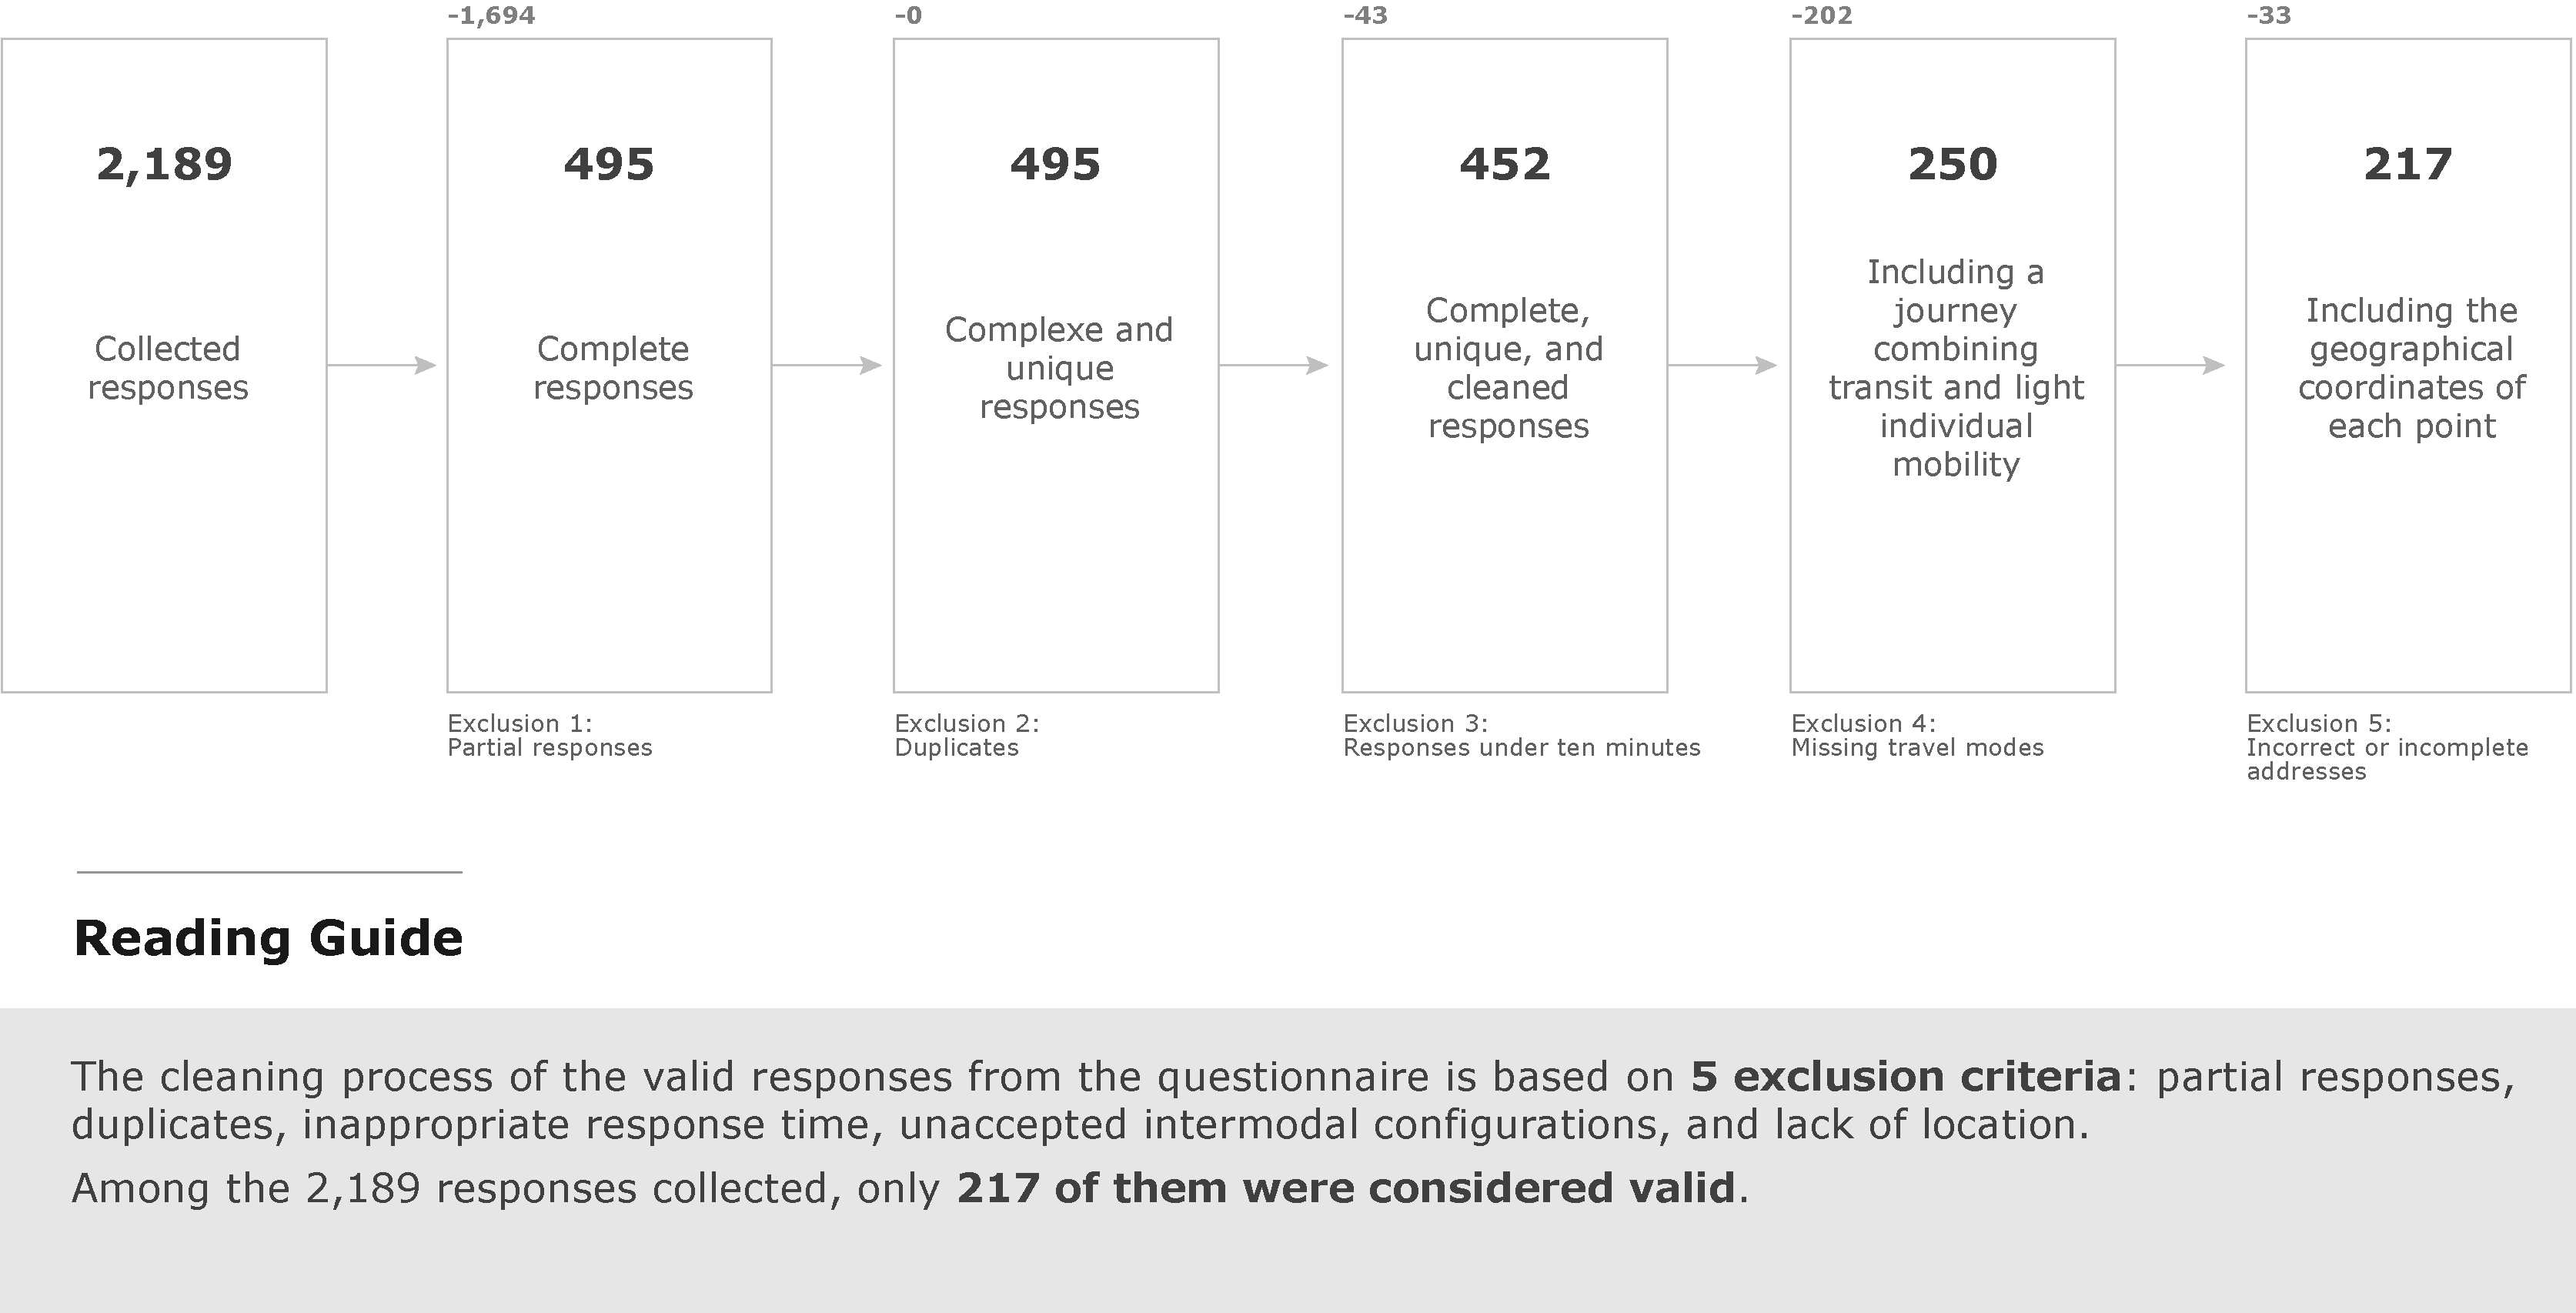
\includegraphics[width=1\columnwidth]{src/Figures/Chap-3/EN_Echantillon_questionnaire.pdf}}
    \vspace{5pt}
    \begin{flushright}\scriptsize{
    Author: \textcolor{blue}{Dylan Moinse (2022)}
    }\end{flushright}
\end{figure}

% Data Cleaning: Exclusion 1 (Partial Responses)
\textsl{First exclusion criterion: partial responses}. The first step of this process involved imputing partial responses \textcolor{blue}{\autocite[12-13]{armoogum_rapport_2018}}\index{Armoogum, Jimmy|pagebf}\index{Tebar, Maria|pagebf}\index{Christian, Barbara|pagebf}\index{Garcia, Cédric|pagebf}\index{Nguyen, Minh-Hieu|pagebf}\index{Rendina, Fabio|pagebf}, resulting in 495 complete responses being retained. As anticipated, a significant proportion of the partial responses were interrupted at the sensitive section dedicated to the spatialization of intermodal trips (\(T_{3}\)). Among the 1,694 incomplete responses (77.39\%), 748 stop precisely at this step, representing 44.15\% of the partial responses. Another critical section can be identified, as 244 responses (14.40\%) stop at the section related to mobility habits and residential aspirations (\(T_{6}\)). This situation seems to be explained, on one hand, by a perceived high cognitive load at the end of the questionnaire, and on the other hand, by a topic perceived as disconnected from the respondents' expectations, based on feedback collected in the open suggestions.%%Translated%%

% Data Cleaning: Exclusion 2 (IP Addresses)
\textsl{Second exclusion criterion: duplicates}. Although 495 responses were initially considered complete, additional exclusion criteria were applied to ensure data quality. Among these criteria was the exclusion of duplicate responses, identified when two or more submissions share the same IP address and contain identical answers. However, after verification, no questionnaire data entry met this exclusion criterion.%%Translated%%

% Data Cleaning: Exclusion 3 (Response Time)
\textsl{Third exclusion criterion: inappropriate response time for the questionnaire}. A third exclusion criterion was applied to maximize the reliability of the collected responses. Submissions with a response time of less than ten minutes were excluded, as this time frame was considered insufficient to thoughtfully complete the questionnaire. Following this step, the final sample was reduced to 452 responses, resulting in the exclusion of 43 complete responses (8.69\%). For informational purposes, the average time recorded for completing the questionnaire was 17 minutes.%%Translated%%

% Data Cleaning: Exclusion 4 (Intermodality)
\textsl{Fourth exclusion criterion: non-compliant intermodal configuration}. This high-impact criterion is related to non-compliance with the eligibility condition for the questionnaire, which requires the described trip to combine a light individual mobility mode with public transport. Despite this instruction, a significant proportion of responses describe trips that do not meet this definition: they typically either describe a trip made exclusively by bike or micromobility, or a monomodal trip alternating between public transport and light individual mobility. This confusion, corroborated by feedback in the open comments, illustrates the difficulty of explicitly addressing the concept of intermodality with users through a digital medium\footnote{~
    In his doctoral thesis on the \Commas{structuring of an integrated meta-network,} \textcolor{blue}{Pierre} \textcolor{blue}{\textcite[41]{ageron_intermodalite-voyageurs_2013}}\index{Ageron, Pierre|pagebf}\index{Varlet, Jean|pagebf} confirms the confusion between plurimodality and intermodality.
}. As a result, 202 responses were excluded on this basis, representing 44.69\% of the sample retained after the application of the first three exclusion criteria. The sample then consists of 250 complete responses.%%Translated%%

% Data Cleaning: Exclusion 5 (Addresses)
\textsl{Fifth exclusion criterion: missing location for one or more landmarks}. The final exclusion criterion applied concerns the geospatialization of intermodal trips. For each response, participants were asked to provide the landmarks for their trips, either as declared addresses or by positioning them on the interactive map, ensuring they were properly referenced and consistent. When anomalies or inconsistencies were detected, such as incorrectly declared addresses or unrealistic geographic locations, the corresponding responses were excluded. This step led to the elimination of 33 responses (13.20\%). After applying the five exclusion criteria, the final sample consists of 217 complete and fully usable responses. These responses describe valid and georeferenced intermodal trips.%%Translated%%

% Sample Description
The final sample, consisting of 217 complete and valid responses, shows a geographical concentration in the Hauts-de-France (54.84\%) and Île-de-France (18.43\%) regions. In contrast, only 7 responses come from participants located outside of France. Regarding participation channels, 65 valid responses (29.95\%) were collected through access to a QR code available on flyers and posters, while the remaining 152 participants (70.05\%) accessed the online questionnaire via digital platforms. From a socio-demographic perspective, 41.47\% of the participants identify as female. This proportion is significantly higher than the sample collected at the train stations (28.21\%) through quantitative observation. However, this proportion, like the other socio-demographic variables of the sample, is closer to data from national surveys on public transport users in France \textcolor{blue}{\autocite[]{enov_enquete_2021}}\index{Enov@\textsl{Enov}|pagebf}.%%Translated%%

% 3.4.2.4.
\needspace{1\baselineskip} % Réserve de l'espace
\subsubsection*{Validation of the Questionnaire Data
    \label{chap3:administration-questionnaire-usagers-validation}
    }

% Coding
The analysis of data from the questionnaire relies on a pre-established structure aimed at translating the respondents' natural language into a usable numerical language (\textcolor{blue}{Olivier} \textcolor{blue}{\textcite[49-62]{martin_analyse_2020}}\index{Martin, Olivier|pagebf}, cited by \textcolor{blue}{François de} \textcolor{blue}{\textcite[89]{singly_questionnaire_2016}}\index{Singly, François de|pagebf}). This coding step leads to the creation of the survey's data file by assigning a code to each response, facilitating subsequent processing and analysis. The coding process can occur at different stages of the questionnaire exploitation: before data entry, during data entry, or after, as explained by \textcolor{blue}{\textcite{ined_saisie_nodate}}\index{Ined@\textsl{Ined}|pagebf}. Some of the codes were adjusted \textsl{a posteriori}, once all responses to the open-ended questions were collected. These textual responses required preliminary work for inventorying, harmonizing, and thematically grouping them. This iterative approach thus allowed for the generation of complementary coding, specifically designed for the quantitative analysis of the questionnaire \textcolor{blue}{\autocite[89]{singly_questionnaire_2016}}\index{Singly, François de|pagebf}.%%Translated%%

% Choice of the Shortest Route
From a geographical perspective, we aimed to project the estimated routes of the 217 valid intermodal trips by focusing on their spatial and temporal distances. This approach is based on the fact that 84\% of respondents reported having \Commas{\textsl{used the shortest path to get to or from the public transport station}} (question \(Q_{03}^{T_{3}}*\)). Assuming that more than four out of five respondents prioritize direct access with minimal detours to various network nodes and targeted destinations, we frame our spatial analysis within the work of \textcolor{blue}{\textcite[2, 7]{qiu_understanding_2022}}\index{Qiu, Xinze|pagebf}\index{Gao, Tianli|pagebf}\index{Yang, Yu|pagebf}\index{Luo, Ankang|pagebf}\index{Shang, Fan|pagebf}\index{Li, Ruiqi|pagebf} who demonstrated such behavior among cyclists in Beijing, Shanghai, and Xiamen, especially during peak hours. This approach also aligns with the reflection of \textcolor{blue}{Frédéric} \textcolor{blue}{\textcite[115]{heran_distances_2009}}\index{Héran, Frédéric|pagebf}, who established that pedestrians and cyclists, relying on their physical strength—i.e., muscular effort—are particularly sensitive to detours and tend to adopt the most direct route. This behavior broadly reflects the \Commas{principle of least effort} defined by the American linguist and philologist \textcolor{blue}{George Kingsley} \textcolor{blue}{\textcite[348]{zipf_human_1949}}\index{Zipf, George Kingsley|pagebf}, a concept focused on minimizing the costs associated with physical and cognitive efforts, to which movement can also contribute \textcolor{blue}{\autocite[348]{zhu_principle_2018}}\index{Zhu, Yueying|pagebf}\index{Zhang, Benwei|pagebf}\index{Wang, Qiuping~A.|pagebf}\index{Li, Wei|pagebf}\index{Cai, Xu|pagebf}.%%Translated%%

% Projection of the Shortest Paths
Taking these elements into account, we projected the routes by prioritizing the most direct path, provided that the routes taken are accessible for the declared mode of transport for each segment. For example, highways were marked as accessible for respondents traveling by car during the feeder or distribution phases, but excluded for pedestrian or light individual mobility modes. In order to overcome the limitation caused by the lack of \acrshort{GPS} flow data, which is often difficult to obtain for personal modes, we based our analysis on the validated geographic coordinates of origin and destination points and the stations crossed. The routes were mapped using the online routing library and tool \Marque{GraphHopper}\footnote{~
    \Marque{GraphHopper 0.13} (\url{https://www.graphhopper.com/}) is an open-source route planning platform, launched in 2019, allowing the calculation of road and public transport routes based on \textsl{OpenStreetMap} data, the \textsl{Shuttle Radar Topography Mission}, and publicly accessible \acrshort{GTFS} data \textcolor{blue}{\autocite{graphhopper_graphhopper_2017}}. Due to its high performance, the engine is mainly used by navigation and logistics applications, but also in accessibility studies.
}, via the \textsl{GraphHopper Maps} mapping interface \textcolor{blue}{\autocite{graphhopper_graphhopper_2017}}\index{GraphHopper@\textsl{GraphHopper}|pagebf}. The geocoding step allowed us to export the routes in \acrfull{GPX} format\footnote{~
    A \acrfull{GPX} file mainly contains waypoints, traces (\textsl{way}), and certain statistical data, such as spatial and temporal distance, altitude, or navigation instructions. This format can be used in \acrshort{GIS} software or \acrshort{GPS} applications.
} and estimate several key indicators, including spatial and temporal distances as well as slope levels for each segment. For example, for the 178 trips made by bike and micromobility recorded among the 217 intermodal trips, we used the \Commas{utility bike} option, set with an average travel speed of 16 kilometers per hour \textcolor{blue}{\autocite[18]{sebban_complementarite_2003}}\index{Sebban, Annie-Claude|pagebf}.%%Translated%%

% Transition
After presenting the methodology implemented to design the questionnaire aimed at collecting data on intermodal trips combining light individual mobility and public transport, it seems relevant to complement this approach with in-depth interviews conducted on small sample sizes. The methodological combination of the questionnaire and the interview provides valuable insights into the fine understanding of these mobility practices, as \textcolor{blue}{\textcite[97]{dureau_lobservation_2014}}\index{Dureau, Françoise|pagebf}\index{Giroud, Matthieu|pagebf}\index{Lévy, Jean-Pierre|pagebf} have experienced. In this perspective, the method of guided tours proves to be highly useful as it allows for capturing the complexity of these practices. It serves as a complementary tool to collect qualitative and \Commas{micro-geographical} data that is directly contextualized \textcolor{blue}{\autocite[109]{bergeron_uncovering_2014}}\index{Bergeron, Julie|pagebf}\index{Paquette, Sylvain|pagebf}\index{Poullaouec-Gonidec, Philippe|pagebf}.%%Translated%%

% ___________________________________________
% 3.5.
\newpage
\needspace{1\baselineskip} % Reserved space
\sectionheader{Description of the Ride-Along Interviews}
\section{Field Interview Survey on Intermodal Practices
    \label{chap3:parcours-commente}
    }

% Introduction 1
Since the early 2000s, the scientific investigation methods used within the \acrfull{HSS} have been profoundly renewed by a paradigm shift, identified by \textcolor{blue}{\textcite[207]{sheller_new_2006}}\index{Sheller, Mimi|pagebf}\index{Urry, John|pagebf} and \textcolor{blue}{\textcite{bonnet_territoires_2000}}\index{Bonnet, Michel|pagebf}\index{Desjeux, Dominique|pagebf} as the \Commas{Mobility Turn} (\textsl{Mobility Turn}). This shift marks a resurgence of mobility-related questions in the social sciences, distinguishing the study of \textsl{movement} from that of \textsl{mobility}. In response to criticisms of research approaches labeled as \Commas{sedentary}, these new methodological perspectives aspire to be as mobile as the phenomena they study \textcolor{blue}{\autocite[207]{buscher_mobile_2009}}\index{Büscher, Monika|pagebf}\index{Urry, John|pagebf}.%%Translated%%

% Introduction 2
This dynamic involves understanding daily movements as constructed and evolving practices, rooted in life trajectories, shaped by a field of possibilities, by what is accessible, and by individual aspirations \textcolor{blue}{\autocite[40]{kaufmann_retour_2014}}\index{Kaufmann, Vincent|pagebf}. In this context, authors such as \textcolor{blue}{Marie-Hélène} \textcolor{blue}{\textcite{massot_mobilites_2010}}\index{Massot, Marie-Hélène|pagebf} emphasize the urgency of designing truly \Commas{mobile} survey methods, capable of overcoming the limitations of \Commas{sedentary} approaches\footnote{~
    The so-called \Commas{sedentary} methods, characteristic of traditional transport research, whether quantitative or qualitative, are often criticized for their inadequacy in addressing the complexity inherent in contemporary mobilities and their multiple dimensions \textcolor{blue}{\autocites[110-111]{buscher_mobile_2009}[178]{merriman_rethinking_2014}}\index{Merriman, Peter|pagebf}\index{Büscher, Monika|pagebf}\index{Urry, John|pagebf}. These sedentary approaches struggle, in particular, to grasp the sensitive and emotional experiences related to mobilities, requiring participants to make a retrospective effort and to verbalize often decontextualized accounts \textcolor{blue}{\autocite[107]{buscher_mobile_2009}}\index{Büscher, Monika|pagebf}\index{Urry, John|pagebf}.
}. Indeed, every movement engages the subject in a dynamic relationship with an environment that constitutes an alterity \textcolor{blue}{\autocite[4]{despres_replacer_2019}}\index{Desprès, Michel|pagebf}\index{Lord, Sébastien|pagebf}\index{Negron-Poblete, Paula|pagebf}. This interaction, structured by various mediations \textcolor{blue}{\autocite[]{freitag_dialectique_nodate}}\index{Freitag, Michel|pagebf}, may manifest in the form of sensory stimuli (\Commas{sensorimotor}), through language (\Commas{symbolic}), or through an interpretation of symbols (\Commas{formalized}).%%Translated%%

% Introduction 3
Understanding the complexity of the depicted social reality requires a transition from static methods to dynamic approaches \textcolor{blue}{\textcite[207]{sheller_new_2006}}\index{Sheller, Mimi|pagebf}\index{Urry, John|pagebf}. From this perspective, it becomes imperative to develop innovative techniques to apprehend the interactions between individuals and territories, while highlighting what is termed \Commas{banal} mobility, associated with everyday life habits \textcolor{blue}{\autocite[1267-1271]{hein_mobile_2008}}\index{Hein, Jane Ricketts|pagebf}\index{Evans, James|pagebf}\index{Jones, Phil|pagebf}. Unlike traditional methods, which often rely on decontextualized data, so-called \Commas{mobile} approaches stand out for their ability to contextualize real-world situations in the studied environment. It is within this framework that a form of methodological hybridization is developed, combining participant observation and field interviews, embodied by the go-along interview device \textcolor{blue}{\autocites[84]{thibaud_methode_2001}[3, 5]{despres_replacer_2019}{meissonnier_methodological_2020}}\index{Desprès, Michel|pagebf}\index{Lord, Sébastien|pagebf}\index{Negron-Poblete, Paula|pagebf}\index{Thibaud, Jean-Paul|pagebf}\index{Meissonnier, Joël|pagebf}. This method is particularly well-suited for capturing the subtleties of sensitive interactions between individuals and their environment, while grounding the analysis in lived experiences and the materiality of places.%%Translated%%

% Annonce du plan
We will begin by defining this original method, outlining its comparative advantages, particularly in relation to traditional interviews, while presenting existing variations and the technical challenges encountered in integrating light individual mobility (see the \hyperref[chap3:parcours-commente-definition]{section dedicated to the definition of the go-along interview}, page~\pageref{chap3:parcours-commente-definition}). The second part of this section is dedicated to how this method has been applied in our work. This includes a comprehensive description of the protocol followed, as well as the presentation of the two go-along interviews conducted and validated (see the \hyperref[chap3:parcours-commente-administration]{section on the methodological protocol of mobile interviews}, page~\pageref{chap3:parcours-commente-administration}).%%Translated%%

% 3.5.1.
\needspace{1\baselineskip} % Reserved space
\subsection{Contextualization of a Mobility \textsl{Being Realized}
    \label{chap3:parcours-commente-definition}
    }

% Définition
One of the \Commas{mobile} methods that has been rapidly gaining popularity over the past fifteen years is the go-along interview method, also known by the English term \textsl{go-along} \textcolor{blue}{\autocite[3]{despres_replacer_2019}}\index{Desprès, Michel|pagebf}\index{Lord, Sébastien|pagebf}\index{Negron-Poblete, Paula|pagebf}. This method relies on a tracking approach that focuses on measuring the evolution and transformation of the experience based on the places crossed and the time elapsed. This ethnographic research tool, based on co-immersion with the participants \textcolor{blue}{\autocite[456]{kusenbach_street_2003}}\index{Kusenbach, Margarethe|pagebf}, offers a rich perspective for exploring the values attributed by users to specific territories. It focuses more specifically on \Commas{lived spaces}, meaning spaces that are not simply traversed but invested with particular meaning by individuals \textcolor{blue}{\autocite[]{fremont_region_1976}}\index{Frémont, Armand|pagebf}. Its main objective lies in collecting \Commas{accounts of perception in motion}, according to \textcolor{blue}{Jean-Paul} \textcolor{blue}{\textcite[83-85]{thibaud_methode_2001}}\index{Thibaud, Jean-Paul|pagebf}, who articulates them around three central methodological hypotheses:
    \begin{customitemize}
\item \textsl{Counter a position of superiority}: this method requires researchers to abandon a posture of \Commas{scholarly and detached observation for an ordinary and engaged description} with their object of study;
\item \textsl{Integrate movement}: movement is placed at the heart of the investigative approach, not only through a \textsl{situated} perception but also a \textsl{moving} perception, reflecting the dynamic interactions with the environment.;
\item \textsl{Articulate \textsl{saying} and \textsl{perceiving}}: this approach relies on verbalized narratives to grasp perception, thus establishing a direct link between lived experience and its narrative translation.
    \end{customitemize}%%Translated%%

% 3.5.1.1.
\needspace{1\baselineskip} % Reserved space
\subsubsection*{Values of Urban Landscape and Participatory Approach in Urbanism
    \label{chap3:parcours-commente-definition-generale}
    }

% Avantage 1
The go-along interview method offers numerous advantages over traditional interviews in mobility studies, as highlighted by \textcolor{blue}{\textcite[3]{despres_replacer_2019}}\index{Desprès, Michel|pagebf}\index{Lord, Sébastien|pagebf}\index{Negron-Poblete, Paula|pagebf}. First, it allows for a finer contextualization of the investigated routes, providing the opportunity to simultaneously observe movements and discourse, a task that is often complex under traditional conditions \textcolor{blue}{\autocite[119]{bergeron_uncovering_2014}}\index{Bergeron, Julie|pagebf}\index{Paquette, Sylvain|pagebf}\index{Poullaouec-Gonidec, Philippe|pagebf}.%%Translated%%

% Avantage 2
Similarly, this approach tends to reduce the hierarchy between the researcher and the participant, by giving participants more control over the course of the interview. This fosters freer and more natural expression, as participants are placed in an active position where they feel more comfortable sharing their personal impressions \textcolor{blue}{\autocite[120]{bergeron_uncovering_2014}}\index{Bergeron, Julie|pagebf}\index{Paquette, Sylvain|pagebf}\index{Poullaouec-Gonidec, Philippe|pagebf}. By guiding the interview, they adopt a stance of autonomous actors, which reduces any potential reluctance to speak \textcolor{blue}{\autocites[264]{carpiano_come_2009}[850]{evans_walking_2011}}\index{Carpiano, Richard~M.|pagebf}\index{Evans, James|pagebf}\index{Jones, Phil|pagebf}.%%Translated%%

% Avantage 3
Furthermore, by allowing participants to take ownership of the interview's flow, this method enables the exploration of topics that, from the researcher's perspective, might seem secondary or unexpected. These issues, often revealed spontaneously, enrich the understanding of mobility dynamics \textcolor{blue}{\autocite[463]{kusenbach_street_2003}}\index{Kusenbach, Margarethe|pagebf}. Finally, the go-along interviews offer great flexibility, allowing the inclusion of past experiences or unforeseen situations that, in a formal and structured interview setting, would likely not have emerged \textcolor{blue}{\autocite[464]{kusenbach_street_2003}}\index{Kusenbach, Margarethe|pagebf}. This ability to capture the unexpected enhances the appeal of this method for capturing the subtleties of social and mobility practices and representations.%%Translated%%

% Micro-géographie
From a geographical perspective, the go-along interview offers the possibility of generating itineraries while representing their progressions and dynamics \textcolor{blue}{\autocite[94]{jones_spatial_2012}}\index{Jones, Phil|pagebf}\index{Evans, James|pagebf}. In this view, landscapes are understood as dynamic scenes, embodying biographical fragments of lived experiences in relation to a territory \textcolor{blue}{\autocite[112]{bergeron_uncovering_2014}}\index{Bergeron, Julie|pagebf}\index{Paquette, Sylvain|pagebf}\index{Poullaouec-Gonidec, Philippe|pagebf}. The richness of the collected information can then be represented in both textual and spatial forms, offering contextualized narratives that account for \Commas{geopoetic} experiences and \Commas{micro-geographical} elements \textcolor{blue}{\autocite[109]{bergeron_uncovering_2014}}\index{Bergeron, Julie|pagebf}\index{Paquette, Sylvain|pagebf}\index{Poullaouec-Gonidec, Philippe|pagebf}. When these perceptions are verbalized in the form of reports, they give rise to what \textcolor{blue}{\textcite[116]{bergeron_uncovering_2014}}\index{Bergeron, Julie|pagebf}\index{Paquette, Sylvain|pagebf}\index{Poullaouec-Gonidec, Philippe|pagebf}, in their article entitled \textsl{Uncovering landscape values and micro-geographies of meanings with the go-along method}, describe as \Commas{micro-geographies of meanings}.%%Translated%%

% SIG et participative
These moving perceptions can also be integrated into representations using \acrshort{GIS}, although this application is still underutilized according to the authors. It thus constitutes a key element in a participatory urbanism approach \textcolor{blue}{\autocite[344]{manzo_finding_2006}}\index{Manzo, Lynne~C.|pagebf}\index{Perkins, Douglas~D.|pagebf}. In the current context, where the integration of population experiences is increasingly central to urban development, this approach aligns with a desire to interpret, understand, and support emerging discourses and practices. This method thus embraces the notion of \Commas{user control}\footnote{~
    \Commas{User control} is a way of giving users an active and decisive role, postulating that practice generates knowledge and expertise. In urban planning, \acrfull{MUS} first appears structurally, as the third term in a set also formed by \acrfull{MOU} and \acrfull{MOE}. It can be described as a process of action based on the legitimate participation of the user, the creation of a formal space, and the recognition of a collective actor, here \Commas{the user expert} \textcolor{blue}{\autocite[73]{vulbeau_maitrise_2014}}\index{Vulbeau, Alain|pagebf}.
} by inviting the respondent to present their usual routes, positioning them as a true expert of their living environment \textcolor{blue}{\autocites[268]{carpiano_come_2009}[1172]{miaux_making_2010}}\index{Carpiano, Richard~M.|pagebf}\index{Miaux, Sylvie|pagebf}\index{Drouin, Louis|pagebf}\index{Morency, Patrick|pagebf}\index{Paquin, Sophie|pagebf}\index{Gauvin, Lise|pagebf}\index{Jacquemin, Christophe|pagebf}. It also aims to anticipate and represent desired futures. However, despite its promising potential, this methodology remains marginally utilized in the field of urbanism \textcolor{blue}{\autocite[120]{bergeron_uncovering_2014}}\index{Bergeron, Julie|pagebf}\index{Paquette, Sylvain|pagebf}\index{Poullaouec-Gonidec, Philippe|pagebf}.%%Translated%%

% 3.5.1.2.
\needspace{1\baselineskip} % Reserved space
\subsubsection*{Modalities and Variants of the Commented Route
    \label{chap3:parcours-commente-definition-variantes}
    }

% Modalités
The modalities of the go-along interview, as a methodological tool, are organized around three major components \textcolor{blue}{\autocites{blanchet_entretien_2015}[7]{despres_replacer_2019}}\index{Desprès, Michel|pagebf}\index{Lord, Sébastien|pagebf}\index{Negron-Poblete, Paula|pagebf}\index{Blanchet, Alain|pagebf}\index{Gotman, Anne|pagebf}:
\begin{customitemize}
    \item \textsl{The scene}. This first component corresponds to what we can call the \Commas{environment of the route}. It constitutes the spatio-temporal framework in which the interview takes place, encompassing both the place and the temporal context in which the exercise occurs, as well as the arrangement of the actors within these spaces;
    \item \textsl{The grid}. The second dimension relates to the \Commas{contractual framework of communication}. It includes the modalities of negotiation concerning the roles assigned to the various actors, the degree of directivity in the interview, the logistical aspects of the accompaniment, and the technical devices employed. These elements define the operational and relational conditions of the route;
    \item \textsl{The actors}. The final aspect concerns intervention strategies, particularly the listening and prompting techniques used by the researcher. These aim to interact with the respondent's discourse, encouraging the emergence of narrative elements while adapting the interview to the specificities of the field.
\end{customitemize}%%Translated%%

% Variantes
The go-along interview has the advantage of being adaptable, with various variants that can be tailored to specific themes. As explained by \textcolor{blue}{\textcite[850]{evans_walking_2011}}\index{Evans, James|pagebf}\index{Jones, Phil|pagebf} and \textcolor{blue}{\textcite[7]{wegerif_ride-along_2019}}\index{Wegerif, Marc~C.A.|pagebf}, it is possible to distinguish typologies based on whether the route is determined by the researcher (guided tours or exploratory walks) or by the respondent (go-along interviews). This \textsl{in situ} interview method can be conducted on foot, by bike, by car, or even by public transport, and applies to both individuals and user groups. Two main categories of go-along interviews emerge \textcolor{blue}{\autocite[456]{kusenbach_street_2003}}\index{Kusenbach, Margarethe|pagebf}: routes undertaken on foot (\textsl{walk-alongs}) and those carried out via a vehicle (\textsl{ride-alongs}).%%Translated%%

% Avantages walk VS ride-alongs
These variants differ not only in their mode of transportation but also in their specific dynamics. According to \textcolor{blue}{\textcite[120]{bergeron_uncovering_2014}}\index{Bergeron, Julie|pagebf}\index{Paquette, Sylvain|pagebf}\index{Poullaouec-Gonidec, Philippe|pagebf}, walking is more directly exposed to sensory stimuli, providing an immersive experience conducive to a rich exploration of the environment. In contrast, car journeys, due to their confined setting, tend to facilitate more intimate verbal exchanges. However, vehicle routes have specific characteristics. On the one hand, they can generate a sense of \Commas{urgency}, related to the speed and pace of movement, contrasting with the slower tempo of walking routes \textcolor{blue}{\autocite[12]{despres_replacer_2019}}\index{Desprès, Michel|pagebf}\index{Lord, Sébastien|pagebf}\index{Negron-Poblete, Paula|pagebf}. This difference echoes the concept of \Commas{adherence} of transportation modes to the urban environment, as defined by \textcolor{blue}{Georges} \textcolor{blue}{\textcite[222]{amar_homo_2016}}\index{Amar, Georges|pagebf}, which emphasizes exposure to the environment. On the other hand, in routes involving a driver, part of the driver’s attention is engaged in the act of driving, causing occasional interruptions in the flow of the interview.%%Translated%%

% 3.5.2.
\needspace{1\baselineskip} % Reserved space
\subsection{Protocol for Sensory Exploration of the Study Area Through Ride-Along Interviews
    \label{chap3:parcours-commente-administration}
    }

% Gap
As highlighted by \textcolor{blue}{\textcite[11]{despres_replacer_2019}}\index{Desprès, Michel|pagebf}\index{Lord, Sébastien|pagebf}\index{Negron-Poblete, Paula|pagebf}, no \textsl{ride-along} study has, to date, been conducted using transportation modes other than the car or bicycle. More generally, go-along interviews conducted by bike remain rare, while those involving micromobility are completely absent. Similarly, intermodal go-along interviews, involving forms of light individual mobility, remain unexplored. This methodological gap offers an opportunity to renew research practices according to the objectives of this study. By prioritizing the use of this approach, this work aims to explore the representations and discourses of intermodal cyclists engaged in intermodal practices, in order to better understand the dynamics and specific issues related to these emerging forms of mobility.%%Translated%%

% Objectifs
This research work specifically aims to gather qualitative information on the practices of users combining the use of public transport networks with forms of light individual mobility. This initiative is original in that it follows the recommendations made by \textcolor{blue}{\textcite[11]{pages_nouveaux_2021}}\index{Pages, Thibaud|pagebf}\index{Lammoglia, Adrien|pagebf}\index{Josselin, Didier|pagebf}. In their prospective study on mobility practices projected for 2030 and 2050 in the Provence-Alpes-Côte d'Azur region, they reported the absence of georeferenced and go-along interviews dedicated to \acrfull{NIEV}. In this regard, \textcolor{blue}{\textcite[13]{gibson_blurred_2021}}\index{Gibson, Hebe|pagebf}\index{Curl, Angela|pagebf}\index{Thompson, Lee|pagebf} recommend that future research adopt mobile methods, such as go-along interviews incorporating the use of videography, in order to explore \acrshort{PeS} practice through the lens of sensory experience. Three main parameters influence the implementation of this research method, and by extension, the relationship between the researcher and the participant:
\begin{customitemize}
    \item \textsl{The environment}. The geographical scope of the study is confined to the administrative boundaries of the Hauts-de-France region, while the temporal sequence is limited to the year 2022, following the distribution of the questionnaire to intermodal travelers;
    \item \textsl{The contractual framework of communication}. The participant, considered an expert of their territory, plays an active role by proposing and guiding the presentation of their lived route. This stance values their experience and mastery of local practices;
    \item \textsl{The modalities of intervention}. The adopted mobile interview is semi-directive, allowing the researcher to guide the discussions while leaving room for spontaneous and unconstrained speech from the participant.
\end{customitemize}%%Translated%%

% 3.5.2.1.
\needspace{1\baselineskip} % Reserved space
\subsubsection*{Integration and Use of Ride-Along Interviews for the Research Topic
    \label{chap3:parcours-commente-administration-methode}
    }

% Recrutement
Participants in the go-along interview were identified following a questionnaire distributed to users. A final question invited respondents to share their contact details for potential follow-up. Among the valid responses collected, 28 individuals expressed their interest in participating in this mobile survey, nearly all of whom were travelers combining the use of traditional bicycles and \acrshort{TER}. The selection of participants was based on an individual analysis of the responses provided by the volunteers. The selection criteria were based on: (i) age; (ii) travel habits; and (iii) informed consent. Thus, for an intermodal cyclist to be recruited for this method, they must (i) be of legal age; (ii) make a regular trip with either the origin or destination located within the Hauts-de-France region; and (iii) agree to be followed and filmed as part of the study, with the assurance that the results will be published respecting anonymity (see \hyperref[annexes:consentement-parcours-commentes]{Appendix~\ref{annexes:consentement-parcours-commentes}}, page~\pageref{annexes:consentement-parcours-commentes}).%%Translated%%

% Technique
Specific instructions were given to participants before conducting the mobile interview. They were invited to make their usual journey to their destination while being followed. During the route, they were asked to share their feelings, experiences, or challenges encountered, whether positive or negative. The users were also given the opportunity to stop at certain points in order to elaborate further on their impressions. The total duration of each go-along interview was set between one and two hours, which is the optimal duration beyond which participants typically show signs of fatigue, as observed by \textcolor{blue}{Margarethe} \textcolor{blue}{\textcite[456, 464]{kusenbach_street_2003}}\index{Kusenbach, Margarethe|pagebf}. In this context, we could intervene occasionally by asking questions to the interviewed individuals to deepen perceptions or clarify certain ideas discussed, in line with the approach adopted by \textcolor{blue}{\textcite[112]{bergeron_uncovering_2014}}\index{Bergeron, Julie|pagebf}\index{Paquette, Sylvain|pagebf}\index{Poullaouec-Gonidec, Philippe|pagebf}. The starting point of the journey was defined by the participant, in accordance with the approach adopted by \textcolor{blue}{\textcite[3]{cox_qualitative_2020}}\index{Cox, Becky|pagebf}\index{Bartle, Caroline|pagebf}, in their work on cyclists with physical disabilities.%%Translated%%

% Matériel
The equipment used is inspired by the work of \textcolor{blue}{\textcite[14]{despres_replacer_2019}}\index{Desprès, Michel|pagebf}\index{Lord, Sébastien|pagebf}\index{Negron-Poblete, Paula|pagebf} who conducted filmed mobile interviews in Montreal using a sports camera and captured the exchanges from a \textsl{verbatim} transcription. The democratization of \acrfull{ICT}—the most prominent in the context of these \Commas{mobile} methods are certainly mobile audio and video recording devices, GPS trackers, and mapping platforms—now available at relatively affordable costs, allows researchers to generate, organize, and analyze field data with a renewed methodological approach \textcolor{blue}{\autocites[1271]{hein_mobile_2008}[120]{bergeron_uncovering_2014}}\index{Bergeron, Julie|pagebf}\index{Paquette, Sylvain|pagebf}\index{Poullaouec-Gonidec, Philippe|pagebf}\index{Hein, Jane Ricketts|pagebf}\index{Evans, James|pagebf}\index{Jones, Phil|pagebf}. Thus, a smartphone equipped with a \acrshort{GPS} tracker was used to geolocate the route followed, in addition to videography, in order to simultaneously capture images and narratives from the participants. This choice was made for a portable and movement-adapted videographic tool: the \Marque{GoPro} sports camera mounted on the bike or the researcher’s \acrshort{PeS}, the same model used by \textcolor{blue}{\textcite[166]{chin_keep_2020}}\index{Chin, Jessica~W.|pagebf}\index{Masucci, Matthew|pagebf}\index{Johnson, Jay|pagebf} to capture the \Commas{emotional rapport} between the body and the bicycle in San José, as part of go-along interviews. This device, also used for quantitative observation (see the \hyperref[chap3:application-observation-quantitative]{section on the application of quantitative observation}, page~\pageref{chap3:application-observation-quantitative}), provides reliability in capturing visual and audio traces, thus facilitating \textsl{a posteriori} analyses. After each go-along interview, the videos were exported for analysis, while the geolocated route was integrated and visualized in a \acrshort{GIS} tool. Finally, the interviews were manually transcribed to ensure the accuracy of the verbal data collected (see \hyperref[annexes:retranscription-pcte1]{Appendices~\ref{annexes:retranscription-pcte1}} and~\ref{annexes:retranscription-pcte2}, pages~\pageref{annexes:retranscription-pcte1} and~\pageref{annexes:retranscription-pcte2}).%%Translated%%

% Format
The adaptation of the go-along interview method to the specific framework of our research topic—the integration of light individual mobility into the public transport system, with a geographical and urban planning approach—leads us to propose an original version of this method. Thus, our go-along interviews are structured in three distinct phases: the access phase, followed by the public transport phase, and then the egress phase. However, this methodological innovation requires a certain technical flexibility, as the equipment is in constant motion and moves from one support to another: at times stabilized on a vehicle, at other times carried and handled directly by the researcher. Nevertheless, this format also has a clear advantage, as it offers participants variations in pace and atmosphere throughout the route. The driving phase, for example, highlights the urban landscape in interaction with the experiences and perceptions expressed by the actor. In contrast, the public transport segment facilitates extended and in-depth exchanges, allowing for revisiting certain points raised earlier. It should be noted that we made sure to adapt our own mobility equipment to that of the interviewed participant in order to fully share the perceptions and experiences they expressed. In other words, we took care to use a bicycle when the participant used that mode of transportation, or a scooter or folding bike, depending on the case.%%Translated%%

% 3.5.2.2.
\needspace{1\baselineskip} % Reserved space
\subsubsection*{Reports from Participants and Their Routes Throughout the Commented Route
    \label{chap3:parcours-commente-administration-participants}
    }

% Echantillon
As part of this doctoral research, the application of this method was limited to an exploratory phase, which included conducting two go-along interviews. This limitation is due to a methodological approach that is primarily complementary to other approaches undertaken, as well as the time-consuming nature of this method. The two ride-along interviews were conducted on March 25 and April 11, 2022, respectively. The first interview, labeled \(PCTE_{1}\), involves a participant using \acrshort{PeS} and \acrshort{TER} to connect two cities in the Nord department. The second route, labeled \(PCTE_{2}\), involves a traveler also using \acrshort{PeS}, but this time in combination with the metro in the Lille metropolitan area.%%Translated%%

    % Tableau description parcours commentés
% Table of Described Routes
%%Translated%%
\begin{table}[h!]
  \centering
  \renewcommand{\arraystretch}{1.5}
  \resizebox{\columnwidth}{!}{
  \begin{tabular}{p{0.27\columnwidth}p{0.3\columnwidth}p{0.35\columnwidth}}
        %\hline
    \rule{0pt}{15pt} \small{\textbf{\textcolor{blue}{Information}}} & \small{\textbf{\textcolor{blue}{Participant \(PCTE_{1}\)}}} & \small{\textbf{\textcolor{blue}{Participant \(PCTE_{2}\)}}} \\
        \hline
    \multicolumn{3}{l}{\textbf{Modal Combination}}\\
\small{Main trip (\(TC\))} & \small{\acrshort{TER} (94.40 km / 72 min)} & \small{Metro (7.9 km / 15 min)}\\
\small{Pre-access trip (\(A\))} & \small{\acrshort{PeS} (1.40 km / 6 min)} & \small{\acrshort{PeS} (1.30 km / 4 min)}\\
\small{Post-access trip (\(E\))} & \small{\acrshort{PeS} (1.50 km / 6 min)} & \small{\acrshort{PeS} (2.3 km / 11 min)}\\
\small{\acrshort{PeS} model} & \small{e-Scooter \Marque{XVY} (\euro200)} & \small{e-Scooter \Marque{Micro} (\euro700)}\\
        \hdashline
    \multicolumn{3}{l}{\textbf{Spatial and Temporal Context}}\\
\small{Date (time)} & \small{April 11, 2022 (7:00 AM)} & \small{March 25, 2022 (8:30 AM)}\\
\small{Rail network} & \small{Lille to Maubeuge (K60)} & \small{Lille to Villeneuve d'Ascq (M1)}\\
\small{\multirow{1.75}{*}{\small{Stations}}} & \small{\multirow{1.75}{*}{\small{Lille Flandres and Maubeuge}}} & \small{République~–~Beaux-Arts and Cité Scientifique Pr. Gabillard}\\
\small{Distances} & \small{97.30 km (84 min)} & \small{11.40 km (30 min)}\\
        \hdashline
    \multicolumn{3}{l}{\textbf{Trip Characteristics}}\\
\small{Purpose} & \small{Professional} & \small{Educational}\\
\small{Frequency} & \small{1 day per week} & \small{2 days per week}\\
\small{Experience} & \small{7 months} & \small{12 months}\\
\small{Network subscription} & \small{SNCF discount card} & \small{Ilévia monthly pass}\\
        \hdashline
    \multicolumn{3}{l}{\textbf{Participant Profiles}}\\
\small{Gender} & \small{Female} & \small{Male}\\
\small{Age} & \small{20 to 25 years} & \small{25 to 30 years}\\
\small{Driver's license} & \small{Category B license} & \small{Category B license}\\
\small{Vehicle} & \small{Personal car} & \small{Personal car}\\
        \hline
        \end{tabular}}
    \caption{Descriptive table of the two go-along interviews.}
    \label{table-chap3:details-parcours-commentes}
        \vspace{5pt}
        \begin{flushleft}\scriptsize{
        \textcolor{blue}{Reading:} The two ride-along interviews were carried out using a personal electric scooter and public transport, between Lille and Maubeuge for the first, and between Lille and Villeneuve d'Ascq for the second.
        }\end{flushleft}
        \begin{flushright}\scriptsize{
        Author: \textcolor{blue}{Dylan Moinse (2022)}
        }\end{flushright}
        \end{table}%%Rédigé%%

% Description générale
We chose to involve these first two participants in order to focus on modes of transportation that not only fall under light individual mobility but are also underexplored in the literature, namely \acrshort{PeS}. This selection also aimed to cover two distinct intermodal combinations: one combining \acrshort{PeS} with \acrshort{TER}, and the other with the metro (see \hyperref[table-chap3:details-parcours-commentes]{Table~\ref{table-chap3:details-parcours-commentes}}, page~\pageref{table-chap3:details-parcours-commentes}). The first participant (\(PCTE_{1}\)) is a relatively recent intermodal commuter, making long daily trips, primarily by private car. However, once a week, she adopts an intermodal practice. For his part, the second participant (\(PCTE_{2}\)) is a student who regularly travels across the Lille metropolitan area. His electric vehicle allows him to connect two distinct destinations several times a week. The choice of these two profiles is also explained by their shared characteristic of being motorized. This feature seemed relevant to enrich our analysis by offering a comparative perspective on modal choices and the partial shift from car use to intermodal practices.%%Translated%%

% Description PCTE1
The first go-along interview (\(PCTE_{1}\)) corresponds to a weekly work commute. It took place between Lille and Maubeuge, combining \acrshort{TER} and \acrshort{PeS}, over a total distance of 97 kilometers completed in 1 hour and 24 minutes. The selected participant, aged 20 to 25 and residing in Lille, holds a driver's license, is motorized, and also owns a personal bicycle. However, she uses an \Marque{XVY} electric scooter, which was given to her by family members with the specific purpose of facilitating the transportation of this vehicle aboard the train. Since acquiring this scooter, the participant has adopted this modal combination for seven months at the time of the interview.%%Translated%%

% Description PCTE1 - rabattement
\textsl{Access segment} (\(PCTE^{A}_{1}\)). The first phase of the trip lasted 6 minutes and covered a distance of 1.4 kilometers, connecting the participant's home to the Lille Flandres station. Although this is a short trip that could be done on foot or by metro, the participant chose to use her \acrshort{PeS}. In fact, she lives in immediate proximity to a metro station that would allow her to reach the station directly in just two stops. However, her modal choice is influenced by several factors. Primarily used in the distribution phase, the scooter is limited to a feeder use. However, its use is also motivated by economic considerations, given the high cost of public transport subscriptions, and practical reasons, such as a walk being too long or the inconveniences related to transfers and waiting times on the metro in Lille and on the bus in Maubeuge. A final determining factor is the perception of a geometric \gls{detour}, caused by the need to temporarily move in the opposite direction of the station using the metro, which weighs heavily on her decision. This aspect will be analyzed in detail in the \hyperref[chap5:detours-pauses-optimisation]{section on strategies for optimizing intermodal chains through geographical and geometric detours} (page~\pageref{chap5:detours-pauses-optimisation}) in \hyperref[chap5:titre]{Chapter~5} (page~\pageref{chap5:titre}). The participant expresses a preference for certain types of cycling infrastructure, such as bus lanes accessible by bicycle, which she finds secure. However, she highlights the danger of mixed lanes with motorized vehicles, particularly on sections with elevation changes that increase speed gaps.%%Translated%%

% Description PCTE1 - TC
\textsl{Train segment} (\(PCTE^{TC}_{1}\)). The second phase of the trip, carried out on \acrshort{TER}, lasted 1 hour and 12 minutes over a distance of 94 kilometers. The overall experience of this segment reflects ambivalence in the participant. On one hand, she appreciates the convenience offered by the heavy rail mode, which allows her to rest without having to drive long distances. The train also provides the opportunity to engage in parallel activities and aligns with her ecological sensitivity regarding mobility. However, a major constraint limits the regular use of this mobility solution: the low frequency of this train service makes it less suitable for the participant's schedule. As a result, the participant uses the \acrshort{TER} relatively infrequently and opts for the occasional purchase of tickets, the cost of which is partially reduced thanks to an annual discount pass. The participant believes that the \acrshort{TER} alone is not a solution suited to her needs: according to her, combined walking is inefficient, while the local public transport network is unreliable and insecure. Moreover, despite her preference for the bicycle, the user acknowledges that the scooter is more practical to carry on the train, thanks to its light weight, its maneuverability on stairs, and its electric assistance for uphill terrain. In the absence of the scooter, the participant states that she would turn exclusively to using the car.%%Translated%%

% Description PCTE1 - diffusion
\textsl{Egress segment} (\(PCTE^{E}_{1}\)). The final phase of the intermodal trip takes place again on \acrshort{PeS}, from the Maubeuge station to the participant's workplace. This route, 1.5 kilometers long and completed in 6 minutes, is marked by a more critical narrative. On this occasion, the intermodal cyclist expresses a lack of confidence in her practice, particularly noticeable through her gestures and the strategies she has gradually implemented. Although the route mostly relies on cycling infrastructure, certain problem areas have been identified. Half of her journey takes place on a bus lane, a type of infrastructure she actually appreciates in Lille. However, in Maubeuge, this recent infrastructure excludes cyclists, with no specific markings visible and traffic lights failing to detect them. This leads her to bypass these constraints, notably by crossing red lights to navigate certain intersections. As she approaches a roundabout, she chooses to cross at the pedestrian crossing to avoid interacting with motor vehicles. Another case reflecting her personal sense of insecurity occurs when she uses a bike lane she deems inadequate due to its narrow width and the downhill curve of the road, which makes it less visible. The design of the infrastructure forces the participant to adopt strategies to minimize risks and discomforts.%%Translated%%

% Description PCTE2
The second go-along interview (\(PCTE_{2}\)) corresponds to a school trip. It was carried out between Lille and Villeneuve d'Ascq, combining the metro and \acrshort{PeS}, over a total distance of 11 kilometers completed in 30 minutes. The participant, aged 25 to 30 and residing in Lille, holds a driver's license and owns a motorized vehicle. However, he prefers to use his \Marque{Micro} scooter, which he bought for daily use. This modal combination is used twice a week in circumstances that will be detailed later. For the past year, the participant has been using this intermodal trip. His case is of particular interest because it is difficult to analyze through a questionnaire. This user performs a chain of trips that he could not do on foot and that he previously made by car (see \hyperref[annexes:retranscription-pcte2]{Appendix~\ref{annexes:retranscription-pcte2}}, page~\pageref{annexes:retranscription-pcte2}).%%Translated%%

% Description PCTE2 - rabattement
\textsl{Access segment} (\(PCTE^{A}_{2}\)). The user is fully aware that his feeder trip, covering a distance of 1.3 kilometers completed in 4 minutes, could be done on foot. Especially since a slightly closer metro stop, Wazemmes, is accessible from his home. Nevertheless, he chooses to go to the République–Beaux-Arts stop, as this option allows him to skip two metro stops and thus reduce his metro travel time, even though it involves traveling a few hundred additional meters on the scooter. Like the first participant, he justifies using his \acrshort{PeS} in the feeder phase primarily because of its increased usefulness during the distribution phase. This section, located in the central neighborhoods of Lille, is, however, perceived negatively by the user due to several obstacles encountered. First, the narrow residential streets, where parking, which had previously been free at that time, significantly reduces the width of the lanes, are considered dangerous. This configuration increases his fear of \Commas{car dooring}, the risk of being hit by an unexpectedly opened car door by a parked driver. Next, his mistrust of two-way bike lanes is exacerbated by the abundance of \acrshort{SUV}\textcolor{blue}{s} traveling in the opposite direction, preventing him from using these lanes as theoretically intended. Finally, although the route taken by the user is not the shortest, this choice is deliberate to avoid cobbled streets, which he considers incompatible with using the scooter.%%Translated%%

% Description PCTE2 - TC
\textsl{Metro segment} (\(PCTE^{TC}_{2}\)). Upon arriving at the departure station, the participant highlights the advantages of his folding vehicle for the metro journey. Thanks to the maneuverability of his \acrshort{PeS}, he is easily able to enter the underground station using the escalators and position himself at the center of the \acrshort{VAL} metro car, where the circulation space is less constrained. However, such a public transport trip, 8 kilometers long or 15 minutes by metro, requires prior adjustment of his time management. The user chooses to adjust his work and study schedule by going earlier to avoid peak periods. He also explains that this mobility equipment increases his resilience in the event of a metro network disruption. In case of a failure, he has an alternative solution, as he is able to complete his entire intermodal journey on the scooter. However, a major difficulty arises at the recently installed metro access gates, which the participant considers unsuitable for travelers with mobility devices or luggage. The traditional gates do not properly detect his passage, forcing him to adopt a strategic position to pass through these barriers without the doors closing on him.%%Translated%%

% Description PCTE2 - diffusion
\textsl{Egress segment} (\(PCTE^{E}_{2}\)). The final part of his intermodal journey, from his exit at the elevated Cité Scientifique–Pr. Gabillard metro station, is divided into two sequences. First, the user heads to a campus building to access his office and collect professional equipment. To do this, he crosses the campus interior to avoid interactions with drivers, even though he considers this space poorly adapted for cyclists. He prefers recently restored paths, although the presence of pedestrians slows him down. This first route, 500 meters long, takes 2 minutes. It is the next segment that justifies the use of the scooter twice a week, as the user must travel to a building on the opposite side of the campus for laboratory experiments. This additional 1.7-kilometer route is completed in 9 minutes using his scooter. He considers such a trip too long on foot and inefficient by metro, as it would require an extra stop followed by walking on both ends, resulting in a total time equivalent to a journey done entirely on foot. Using the scooter thus allows him to optimize his time, particularly for making the round trip and returning to his office after classes to drop off his belongings or continue his work. However, this campus route is not described as pleasant by the participant. He points out several obstacles that make the cycling experience less fluid: the traffic lanes lack appropriate cycling infrastructure, including one-way streets that are not cycle-friendly and dangerous intersections, as well as the systematic presence of gates that force him to bypass these obstacles by riding on the sidewalks.%%Translated%%

% ___________________________________________
% 3.*.
\newpage
\needspace{1\baselineskip} % Reserved space
\addcontentsline{toc}{section}{Conclusion of Chapter~3}
\sectionheader{Conclusion of Chapter~3}
\section*{Conclusion of Chapter~3
    \label{chap3:conclusion}
    }
    \markright{Conclusion of Chapter~3}{} 

% Conclusion générale
The methodology developed in our doctoral research follows a logic of complementarity between quantitative and qualitative approaches, aiming to address the challenges of a topic as multidimensional as the urban model of \acrshort{TOD}, revisited through the lens of emerging light individual mobility. The methodological structure is based on an articulation between direct observation tools, surveys through questionnaires and \textsl{in situ} interviews, as well as geostatistical analyses, enabling the exploration of the complexity of daily mobility and the interrelationships between networks and territories. In this regard, the approach adopted in our research evokes, for example, the one developed in \textcolor{blue}{Adrien} \textcolor{blue}{\textcite{poisson_amenagements_2019}}\index{Poisson, Adrien|pagebf}\index{Chapelon, Laurent|pagebf}\index{Lammoglia, Adrien|pagebf}’s thesis—entitled \textsl{Cycling Infrastructure as a Lever for Modal Shift in Favor of Bicycle Use: The Case of the Montpellier Metropolitan Area} and conducted at \acrfull{LAGAM}—which relied on an online questionnaire conducted in 2021, allowing for the mapping of routes taken by cyclists, followed by the implementation of go-along interviews. This reflects a trend in mobility research towards mixed methodologies tailored to the specificities of each context. The regional territorial analysis, focused on stations as interconnection hubs, provided the basis for implementing our methodological path. By prioritizing a \Commas{customized} survey, we aimed to go beyond the often compartmentalized \Commas{classic} approaches, in order to grasp the complex interactions between territorial and social dimensions. In this sense, we aimed to move beyond traditional dichotomies between normative and descriptive approaches. This methodological hybridization thus seeks to contribute to the renewal of analytical frameworks while opening perspectives for a better integration of mixed research in \acrshort{TOD} studies.%%Translated%%

% Terrain géographique et contours méthodologiques
In addition to this multidimensional approach, the choice of a regional geographic scope, centered on the Hauts-de-France, and the mapping of station neighborhoods reflect a desire to adopt a multiscalar perspective suited to the complexity of the concept of urban planning. As we have seen, our methodological orientation is based on an articulation between regional and local scales. At the regional scale, the aim is to consider the Hauts-de-France as a privileged study laboratory, due to its potential for regional development oriented toward public transport. At the local scale, the station neighborhoods, designed as spaces theoretically accessible on foot or by light individual mobility, constitute ideal grounds for observing interactions between infrastructure, urban systems, and mobility behaviors. The multiscalar approach thus developed allows us to move beyond a strictly local or macro-regional view, capturing the complexity of mobility systems and urban dynamics. It also provides interpretive frameworks for a better understanding of the relationships between mobility, urban planning, and individual behaviors. Finally, this methodological reflection was enriched by a reflexive stance on the role of the researcher and their relationship to the field. This allowed us to objectify our approach while adhering to ethical principles throughout our investigation. This introspection also contributed to a better understanding of the limits of our method, particularly in terms of the generalization of the results obtained.%%Translated%%

% Apports de l'observation quantitative
As we will see in the following chapters of this document, the statistical results from the quantitative observation will allow us to characterize the \Commas{emerging} nature of light individual mobility (\hyperref[chap4:proportion-croissante-voyageurs-intermodaux]{section on the growing proportion of intermodal cyclists}, page~\pageref{chap4:proportion-croissante-voyageurs-intermodaux} of \hyperref[chap4:titre]{Chapter~4}, page~\pageref{chap4:titre}). These data will provide us with the means to create a socio-demographic profile of these users, taking into account variables such as gender and age (\hyperref[chap4:demographie]{section on the profile of intermodal travelers}, page~\pageref{chap4:demographie} of \hyperref[chap4:titre]{Chapter~4}, page~\pageref{chap4:titre}). Finally, station observation will allow us to model gender differences in intermodal practices, while establishing associations with the characteristics of the urban environment, whether measured or perceived (\hyperref[section-chap4:cyclabilite-genre]{section on the moderating role of bikeability on gender inequalities}, page~\pageref{section-chap4:cyclabilite-genre} of \hyperref[chap4:titre]{Chapter~4}, page~\pageref{chap4:titre}).%%Translated%%

% Apports du questionnaire
As for the questionnaire, it will allow us to deepen the characterization of individuals by taking into account their social status and their travel habits (\hyperref[chap4:capital-economique-culturel]{section on the economic and cultural capitals of intermodal cyclists}, page~\pageref{chap4:capital-economique-culturel} of \hyperref[chap4:titre]{Chapter~4}, page~\pageref{chap4:titre}). The routes mapped from the collected responses will offer us a dual perspective. On one hand, they will help identify the distances considered socially acceptable for cycling and micromobility (\hyperref[chap5:aire-secondaire-quartier-gare]{section on the extension of station neighborhoods}, page~\pageref{chap5:aire-secondaire-quartier-gare} of \hyperref[chap5:titre]{Chapter~5}, page~\pageref{chap5:titre}). On the other hand, they will allow us to quantify improvements in accessibility potential to urban amenities (\hyperref[chap5:accessibilite-intermodale-extension-aire-influence]{section on intermodal accessibility gains}, page~\pageref{chap5:accessibilite-intermodale-extension-aire-influence} of \hyperref[chap5:titre]{Chapter~5}, page~\pageref{chap5:titre}). Moreover, these analyses will help identify mobility strategies based on practices of detour and \gls{break} (\hyperref[chap5:detours-pauses-optimisation]{section on the spatiotemporal optimization of intermodal movements}, page~\pageref{chap5:detours-pauses-optimisation} of \hyperref[chap5:titre]{Chapter~5}, page~\pageref{chap5:titre}). Finally, the spatialization of different types of station neighborhoods, based on the analysis of data collected on the intermodal use of light individual mobility, will allow the development of a regional model. This model will take into account the levels of development and the articulation between transport nodes and the layout of expanded station neighborhoods (\hyperref[chap6:titre]{Chapter~6}, page~\pageref{chap6:titre}).%%Translated%%

% Apports du parcours commenté
As for the go-along interview, although we are aware of the limitations related to the small sample size and its exploratory nature, this methodological tool will allow us to enrich the quantitative analyses with illustrations. These will not only deepen the insights drawn from our empirical material but also provide additional information to help understand the identified behaviors. In this regard, the go-along interview will be used, in particular, to examine the role of factors influencing the gendered use of bicycles and micromobility (\hyperref[section-chap4:cyclabilite-genre]{section on the moderating role of bikeability on gender inequalities}, page~\pageref{section-chap4:cyclabilite-genre} of \hyperref[chap4:titre]{Chapter~4}, page~\pageref{chap4:titre}). Moreover, this \Commas{sensitive} method will help clarify certain mobility strategies in the form of detours and pauses (\hyperref[chap5:detours-pauses-optimisation]{section on the spatiotemporal optimization of intermodal movements}, page~\pageref{chap5:detours-pauses-optimisation} of \hyperref[chap5:titre]{Chapter~5}, page~\pageref{chap5:titre}).%%Translated%%

% ___________________________________________
     \newpage
     
% Valorisation scientifique
    \begin{tcolorbox}[colback=white!5!white,
                      colframe=blue!75!blue,
                      title=Valorization
                      \\
                      Chapitre~3]
\Large{\textcolor{blue}{\textbf{Seminars:}}}
    \\\\
\small{\textcolor{blue}{\textcite{moinse_mise_2023}}. La mise en pratique de parcours commentés en micro-mobilités : Interroger les pratiques intermodales inscrites dans des quartiers de gare de la région Hauts-de-France. \textsl{20 ans du LVMT}. \Commas{Interroger et représenter les territoires à partir des expériences individuelles: L’apport des méthodes sensibles}, Paris.
\\
\footnotesize{\url{https://shs.hal.science/halshs-04034957}} (\textbf{C-COM})}
    \\\\
\small{\textcolor{blue}{\textcite{moinse_analyse_2022}}. L'analyse qualitative des pratiques intermodales et des configurations urbaines des quartiers de gare : La mise en œuvre de parcours commentés en trottinette électrique dans la région Hauts-de-France. \textsl{Journée Doctorale SESAM}, La mobilité, un enjeu interdisciplinaire, Villeneuve d'Ascq.
\\
\footnotesize{\url{https://shs.hal.science/halshs-03654175}} (\textbf{C-COM})}
    \\\\
\Large{\textcolor{blue}{\textbf{Communication:}}}
    \\\\
\small{\textcolor{blue}{\textcite{lehmann_methodes_2023}}. Les méthodes sensibles au service de l’aménagement urbain \textsl{Ingenius}. 
\\
\footnotesize{\url{https://ingenius.ecoledesponts.fr/articles/les-methodes-sensibles-au-service-de-lamenagement-urbain/}}}
    \end{tcolorbox}

    % ___________________________________________
    % Subbibliography
    \newpage
    \sectionheader{Bibliography of Chapter~3}
    \begingroup
    \renewcommand{\bibfont}{\scriptsize}
\printbibliography[segment=\therefsegment, heading=subbibintoc, title={Bibliography of Chapter~3}, label=chap3:bibliographie]
    \endgroup
    \end{refsegment}